\chapter{Higgs Boson Properties in $ZZ\rightarrow4\ell$}
\label{sec:properties}
\chaptermark{Properties}

\begin{center}
\begin{footnotesize}
\textit{1 The world is all that is the case. \\
1.1 The world is the totality of facts, not things.\\
1.2 The world divides into facts.}\\
Ludwig Wittgenstein, ``Tractatus Logico-Philosophicus"
\end{footnotesize}
\end{center}

\section{Prelude to Property Measurements}
\label{sec:Prelude}

With a Higgs-like resonance discovered, we analyzed and quantified many properties of the new particle, each of which will be covered in the following sections. Each property measurement uses the same base analysis (i.e. same data, same object definitions, same selection requirements, etc.) as in Sec.~\ref{sec:discovery}, with small additions or modifications as needed. Anything that has changed will be listed explicitly. Each of the following property measurements\footnote{Except Sec.~\ref{sec:OffShellAnom}, where a paper is moving through the approval process at the time of this thesis.} is based on a published paper, cited for further reference. Where applicable, the following measurements were combined with other decay channels. The final results of those combinations will be discussed briefly in each instance.

In Sec.~\ref{sec:HighMass}, a search for additional Higgs bosons was performed \cite{Khachatryan:2015cwa}, which requires a few modifications to how a signal would appear compared to the exclusion limit set for a SM Higgs boson. In Sec.~\ref{sec:SpinParity}, the spin-parity of the new resonance was tested against alternative spin states \cite{Khachatryan:2014kca}. In Sec.~\ref{sec:Width} we reinterpreted the high mass region into a search for an off-shell enhancement to the Higgs boson $m_{4\ell}$ shape \cite{Khachatryan:2014iha}. As we will see, this equates to an upper bound on the width of the new particle, which constrains its ability to decay to yet-unobserved physics. Lastly, in Sec.~\ref{sec:OffShellAnom}, the width measurement can be utilized to set a limit on the last anomalous coupling not covered in Sec.~\ref{sec:SpinParity}.

\section{High Mass Higgs Search}
\label{sec:HighMass}

In light of the exclusion limits set in Sec.~\ref{sec:ZZ4lResults}, where the SM Higgs boson was excluded in the range $129.5<m_H<832.0$ $\rm{GeV}$, why repeat the search? As discussed in Chapter 13 of \cite{HXSWG_Properties}, although there is a Higgs-like resonance at $125.6$ $\rm{GeV}$, if its signal strength was below the expectations of the Standard Model it may not fully explain the mass generation of other particles. In this instance, an additional higher mass particle would be required to complete this picture. One such model is called the \textit{Electroweak Singlet model}\footnote{So named by the necessity of a new scalar field that would couple to the electroweak sector and acquire a non-zero vacuum expectation energy, similar to the Higgs field.} (EWS). Although both CMS and ATLAS observe a Higgs boson near $125$ $\rm{GeV}$, signal strengths of $\mu<1$ are not excluded so this model is not unreasonable. Additionally, any observed particle in the high mass region would instantly become a very promising candidate for dark matter.

In the EWS model, both the observed $125.6$ $\rm{GeV}$ Higgs boson and any high mass partner would couple to fermions and bosons in the same way as the SM Higgs mechanism, but with modified signal strengths compared to SM predictions. To account for this in the search, the signal line shape used in the high mass region ($140-1000$ $\rm{GeV}$ for this analysis) is altered slightly from what is defined in Sec.~\ref{sec:ZZ4lMassShape}. The heavier particle, hereafter called $H$ where $h$ is the $125.6$ $\rm{GeV}$ particle, adopts different parameters to correct for the lower signal strength and to account for new decay channels\footnote{Consider the case where $m_{H} > 2\times m_{h}$. In this case, $H\rightarrow hh$ may be possible.}. Defining $C$ and $C'$ as the scale factors compared to the SM signal strengths for $h$ and $H$ respectively, the total signal strength agrees with the standard model by construction: $C^2 + C'^2 = 1$. Then, the signal strength and width of $H$ become
\begin{align}
\mu' &\equiv \mu_{H} = C'^2 (1-\mathcal{B}_{\rm{new}}) \\
\Gamma' &\equiv \Gamma_{H} = \Gamma_{SM}\frac{C'^2}{1-\mathcal{B}_{\rm{new}}}
\end{align} 
where $\mathcal{B}_{\rm{new}}$ is the branching ratio of $H$ to new decay channels.

As discussed in Sec.~\ref{sec:ZZ4lMassShape}, Higgs boson signals below $400$ $\rm{GeV}$ have sufficiently small widths that the shape can be embodied by just a Briet-Wigner function convoluted with a Double Crystal Ball whereas shapes for masses above $400$ $\rm{GeV}$ must be treated with the Complex Pole Scheme. This remains true in the high mass search, but there is the additional complication of non-negligible interference between the signal and background \cite{Passarino:2012ri} requiring explicit modifications to the signal distributions obtained without interference\footnote{Because the interference is non-negligible at high masses, this means that signal-only shapes for $H\rightarrow 4\ell$ are limited approximations and thus non-physical, even for $m_{H}<400$ $\rm{GeV}$. However, as the effects of this interference only become relevant for $m_{4\ell} > 2\times m_{Z} \gg 125.6$ $\rm{GeV}$, this does not weaken the discovery.}. Unfortunately, at the time of this analysis, though there were MC generators to make signal-only samples at NLO, MC generators that account for the combined effects of signal, background, and interference only existed at LO.

For ggF, {\tt GG2VV} was used to generate signal-only (S), background-only (B), and combined signal and background with interference samples (BSI). By generating a background sample plus a combined sample and a signal sample for the same $m_H$, the shape of interference can be found at LO via subtraction: (Signal+Background+Interference) - (Signal) - (Background) will give the Interference if all samples are weighted by their respective cross sections. But, this interference is only LO, while cross sections are known for signal up to NNLO. To account for this, as discussed in \cite{HXSWG_Properties}, a scale factor can be introduced to rescale interference to NNLO, but there is disagreement as to what should be rescaled. One method scales the leading order signal distribution up to NNLO by itself while background and interference are left at LO (\textit{additive method}). Alternatively, the combination of the leading order signal and interference could be scaled by a factor related to the NNLO signal (\textit{multiplicative method}). Instead, this analysis uses an intermediate method for the nominal shape, while the additive and multiplicative methods are used as shape systematics.

To find these interference shapes, it is too computationally intensive to make the signal-only and BSI sample for every mass point, so an analytic shape is built to model interference for different values of $m_{H}$ and $C'^2$ which is then applied to the modified Breit-Wigner $m_{4\ell}$ shapes discussed in Sec.~\ref{sec:ZZ4lMassShape}. For the EWS $m_{4\ell}$ shapes, this interference is assumed to scale based on the modified coupling such that $(\mu + I)_{\rm{BSM}} = \mu_{\rm{SM}}C'^2 + I_{\rm{SM}}C'$. Lastly, a double-sided Crystal Ball function is again convoluted with these $m_{4\ell}$ shapes to account for resolution effects. 

The same process for ggF is pursued for VBF $m_{4\ell}$ shapes, including interference, with the caveat that the LO generator {\tt Phantom} cannot generate a signal-only VBF samples. Instead, two BSI samples are generated: one with $\mu=\mu_{SM}$ and another with $\mu=25\times\mu_{SM}$. While the signal scales linearly with the signal strength, the interference scales as the square root, that is $BSI_{25\times\mu_{SM}} = 25\times S_{SM} + 5\times I_{SM} + B_{SM}$. With these two samples and a background-only sample, interference can be extracted for reweighting.

There is one last modification from the analysis of Sec.~\ref{sec:discovery}. As VBF becomes increasingly important for higher masses (see Sec.~\ref{sec:HiggsProduction}), so instead of using a linear discriminant for the dijet category, a full matrix element approach, \textit{vbfMELA}, is used to separated VBF from gluon fusion with two radiated jets (see Sec.~\ref{sec:VBFVertex}). The new discriminant is 
\begin{equation}
\mathcal{D}_{\rm{jet}}=\frac{\mathcal{P}_{\rm{VBF}}}{\mathcal{P}_{\rm{VBF}} + c(m_{4\ell})\times \mathcal{P}_{\rm{H+jj}}}
\end{equation}
where the $\mathcal{P}_{\rm{VBF}}$ and $\mathcal{P}_{\rm{H+jj}}$ are probabilities coming from JHUGen matrix elements and $c(m_{4\ell})$ is used to equalize the total probability above and below $\mathcal{D}_{\rm jet}=0.5$, similar to $\mathcal{D}_{\rm{bkg}}^{\rm{kin}}$ in Sec.~\ref{sec:ZZ4lKD}. This vbfMELA discriminant has a relative improvement of 25-30\% over the earlier linear discriminant of Eqn.~\ref{eq:HiggsFisher}, seen in the efficiency curves of Fig.~\ref{fig:vbfMELAROC}. Performance of this discriminant was shown to be in agreement with a BDT technique trained over the same production variables, but the MELA approach is motivated directly from a physical argument and will provide a path for other applications (e.g. Sec.~\ref{sec:OffShellAnom}).

\begin{figure}[htbp]
\begin{center}
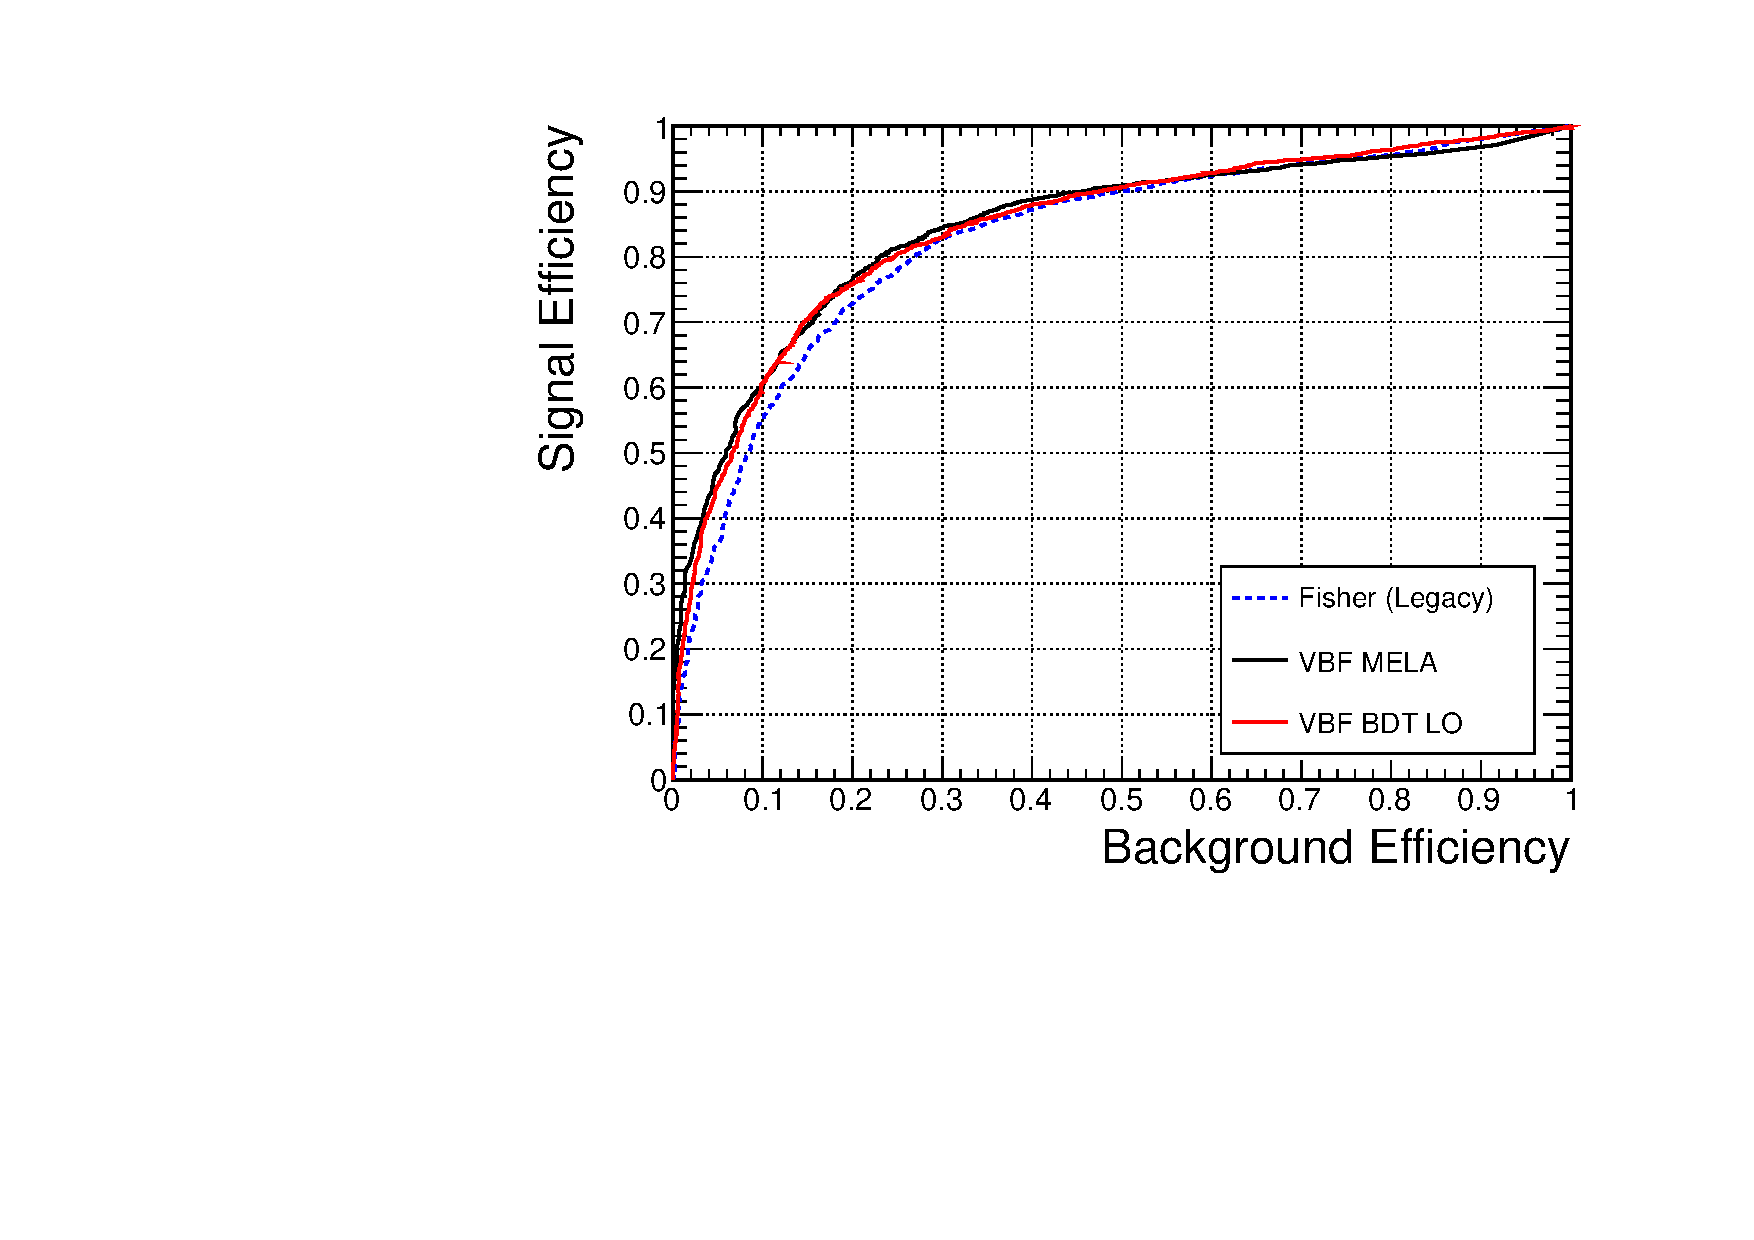
\includegraphics[width=.6\linewidth]{HiggsProperties/figures/BDTROC_vbf.pdf}
\caption[Improvement of the $\mathcal{D}_{\rm{jet}}$ Discriminant Using MELA Techniques]{Efficiency curves showing the relative performance of the linear discriminant (in dashed blue, labeled Fisher), the vbfMELA discriminant (black) constructed from the production angles, and a BDT (red) trained on the same production variables. The vbfMELA discriminant shows improved performance over the linear discriminant and the BDT method shows similar performance as vbfMELA.}
\label{fig:vbfMELAROC}
\end{center}
\end{figure}

Otherwise, the statistical analysis is largely identical to Sec.~\ref{sec:ZZ4lAnalysis}. Two-dimensional templates of $(\mathcal{D}_{\rm{jet}},m_{4\ell})$, such as those seen in Fig.~\ref{fig:vbfMELATemplates}, are made using their respective MC samples (or control region for $Z+X$). For ggF, MINLO is now used to populate the templates as it is known to have more accurate jet kinematics. For VBF, newer samples from {\tt POWHEG} 1.5 which account for the Complex Pole Scheme are used. A new background-only sample from VBF processes is generated via {\tt Phantom}. The decay of this sample approximately matches the dominant $q\bar{q}\rightarrow ZZ$ background while the $p_{T}$ matches VBF, used in the 0 and 1 jet categories respectively. All other MC samples are identical to Sec.~\ref{sec:ZZ4lMCandData}.

\begin{figure}[htbp]
\begin{center}
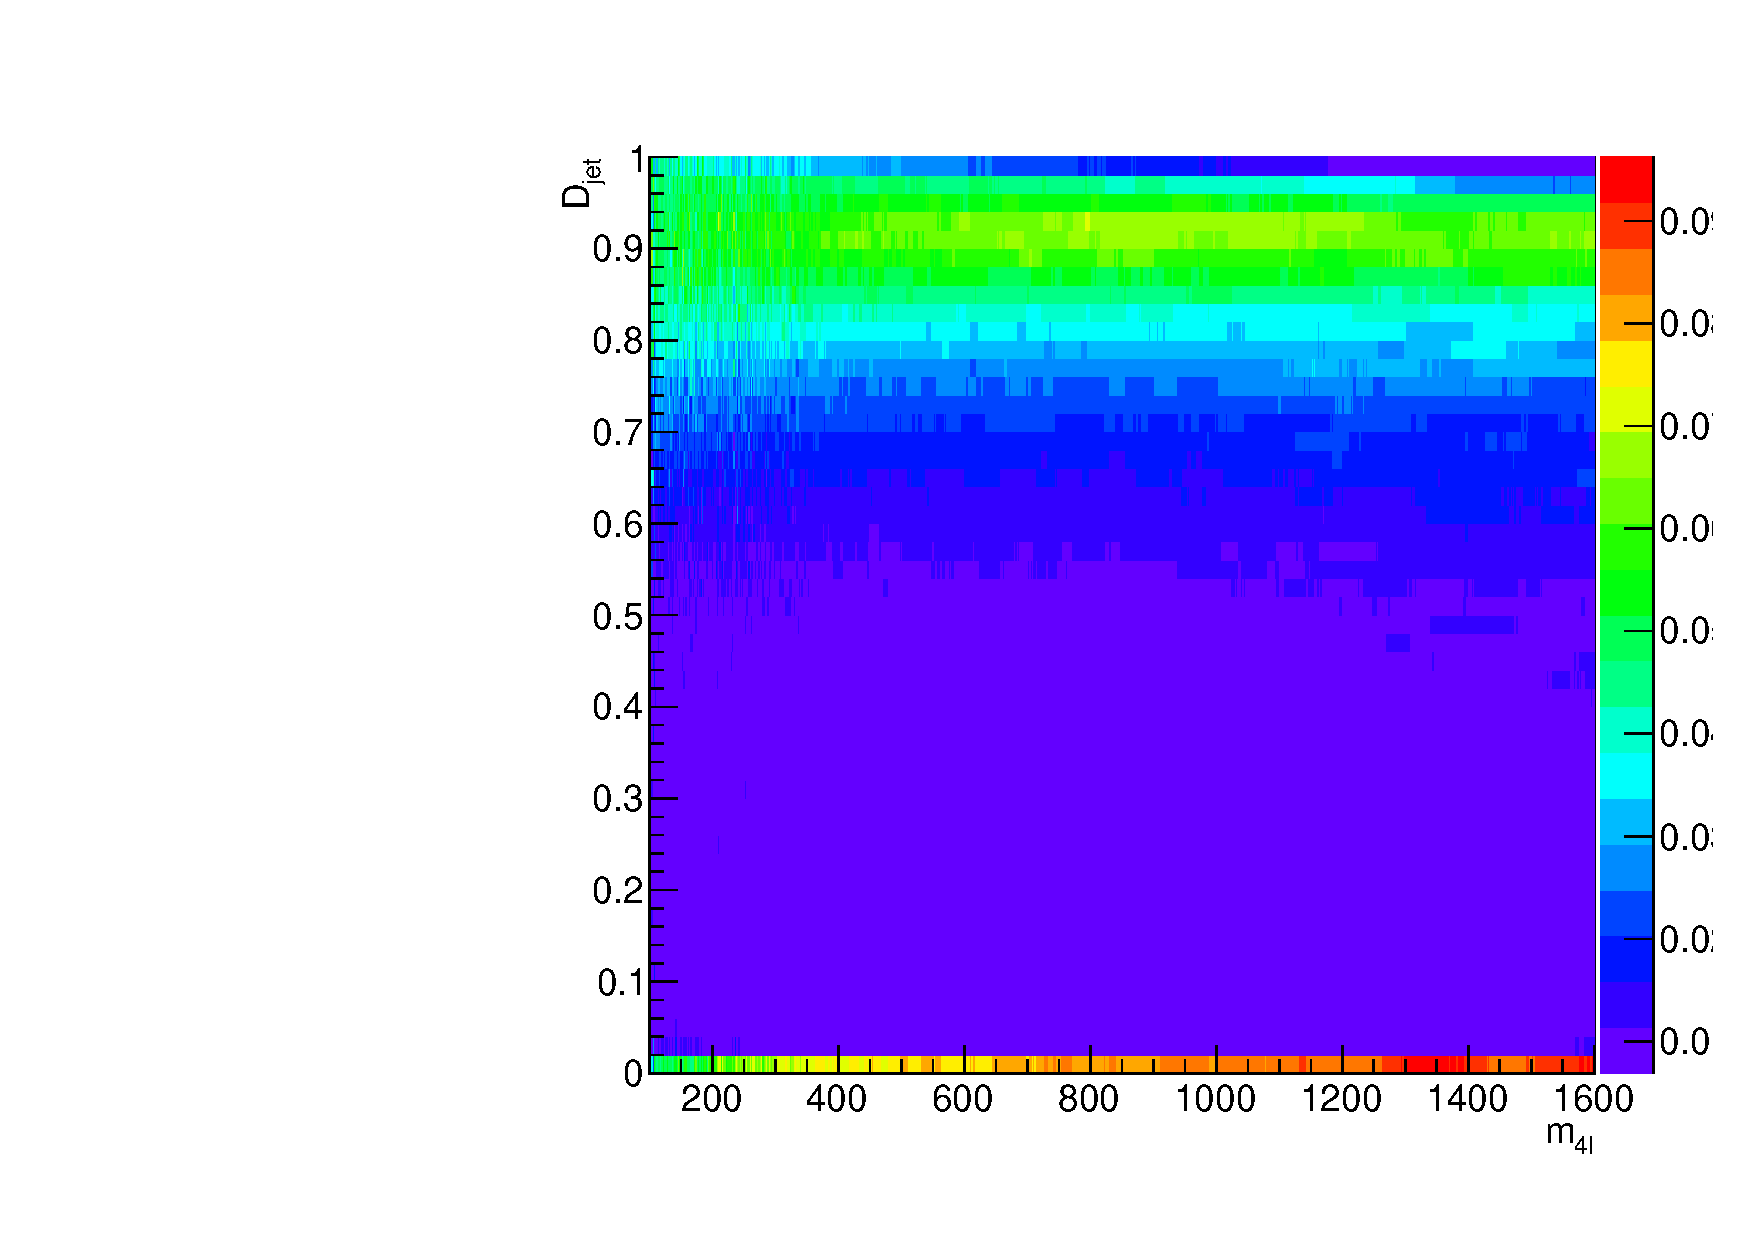
\includegraphics[width=.3\linewidth]{HiggsProperties/figures/qqH_Djet_template.pdf}
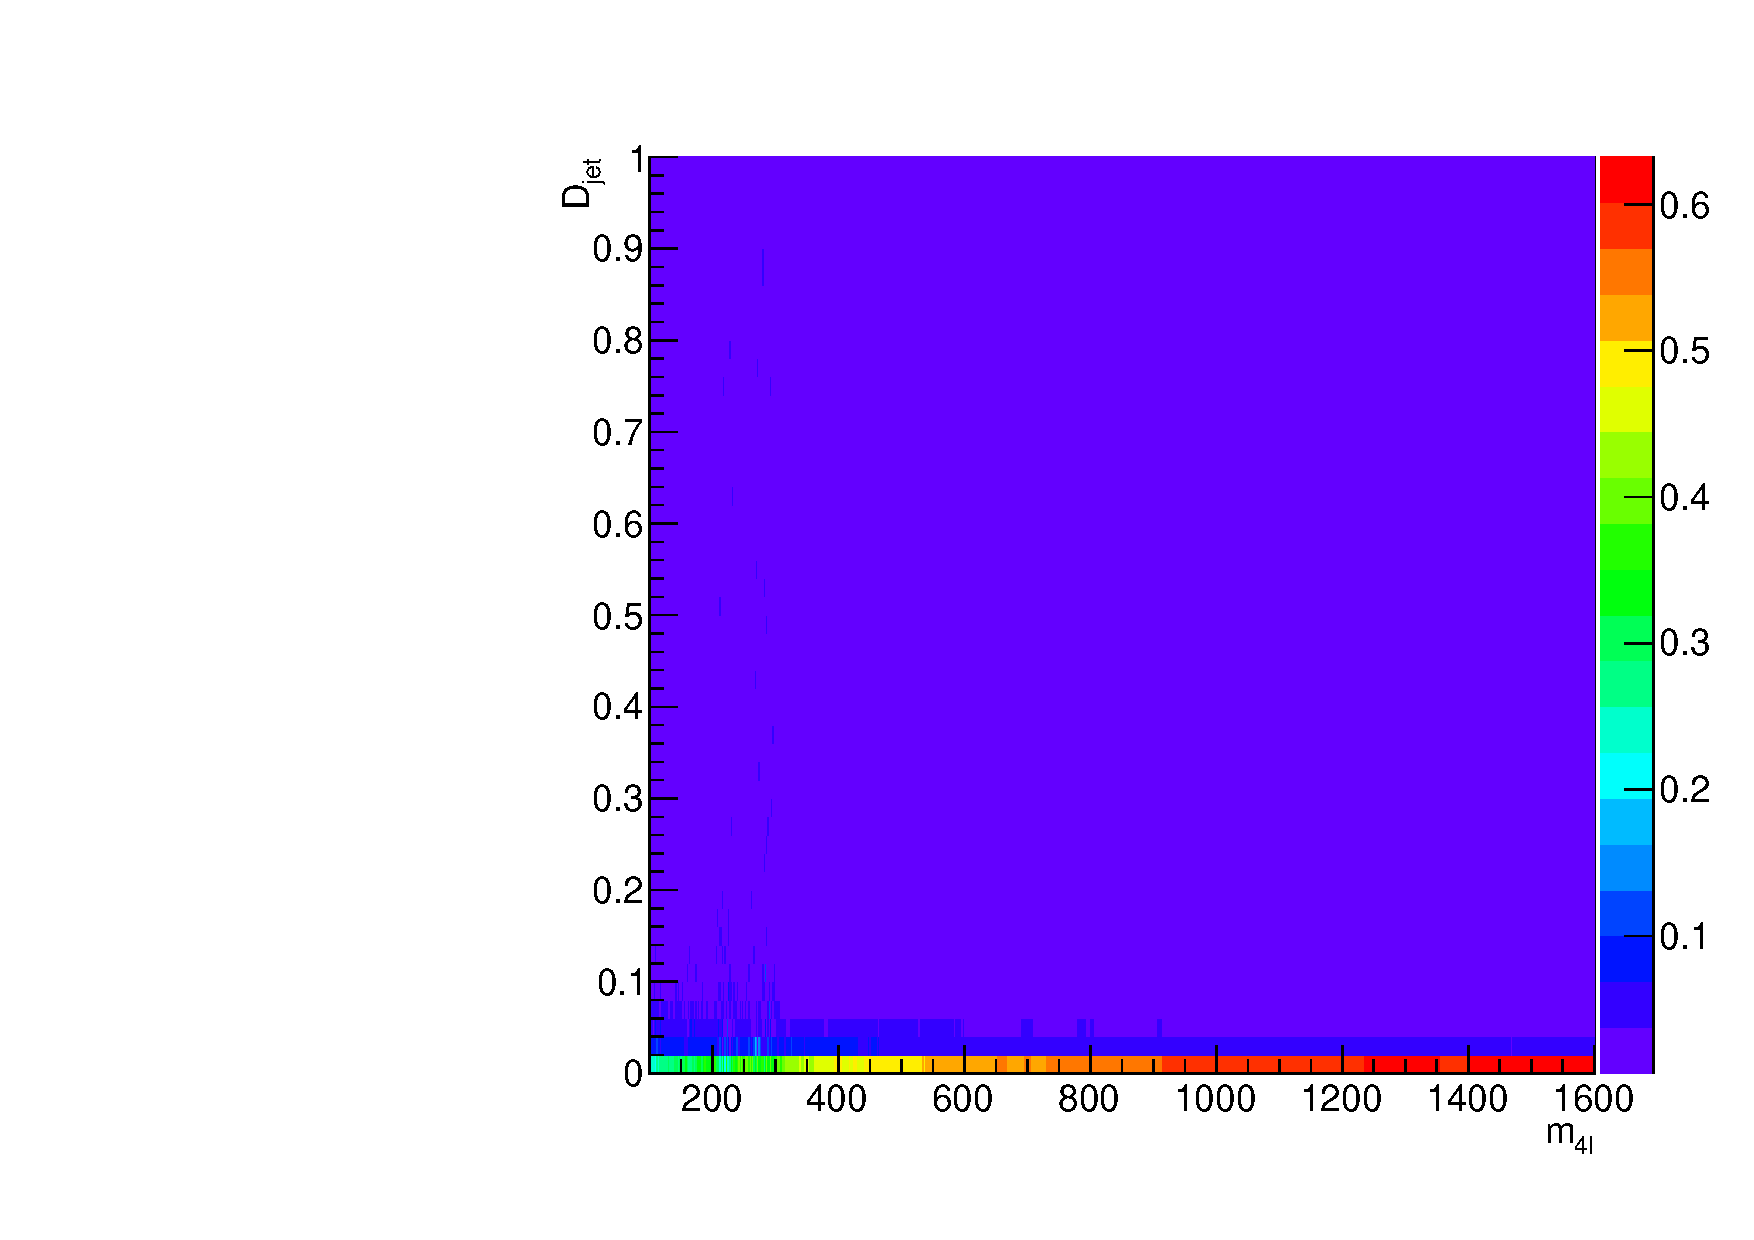
\includegraphics[width=.3\linewidth]{HiggsProperties/figures/ggH_Djet_template.pdf}
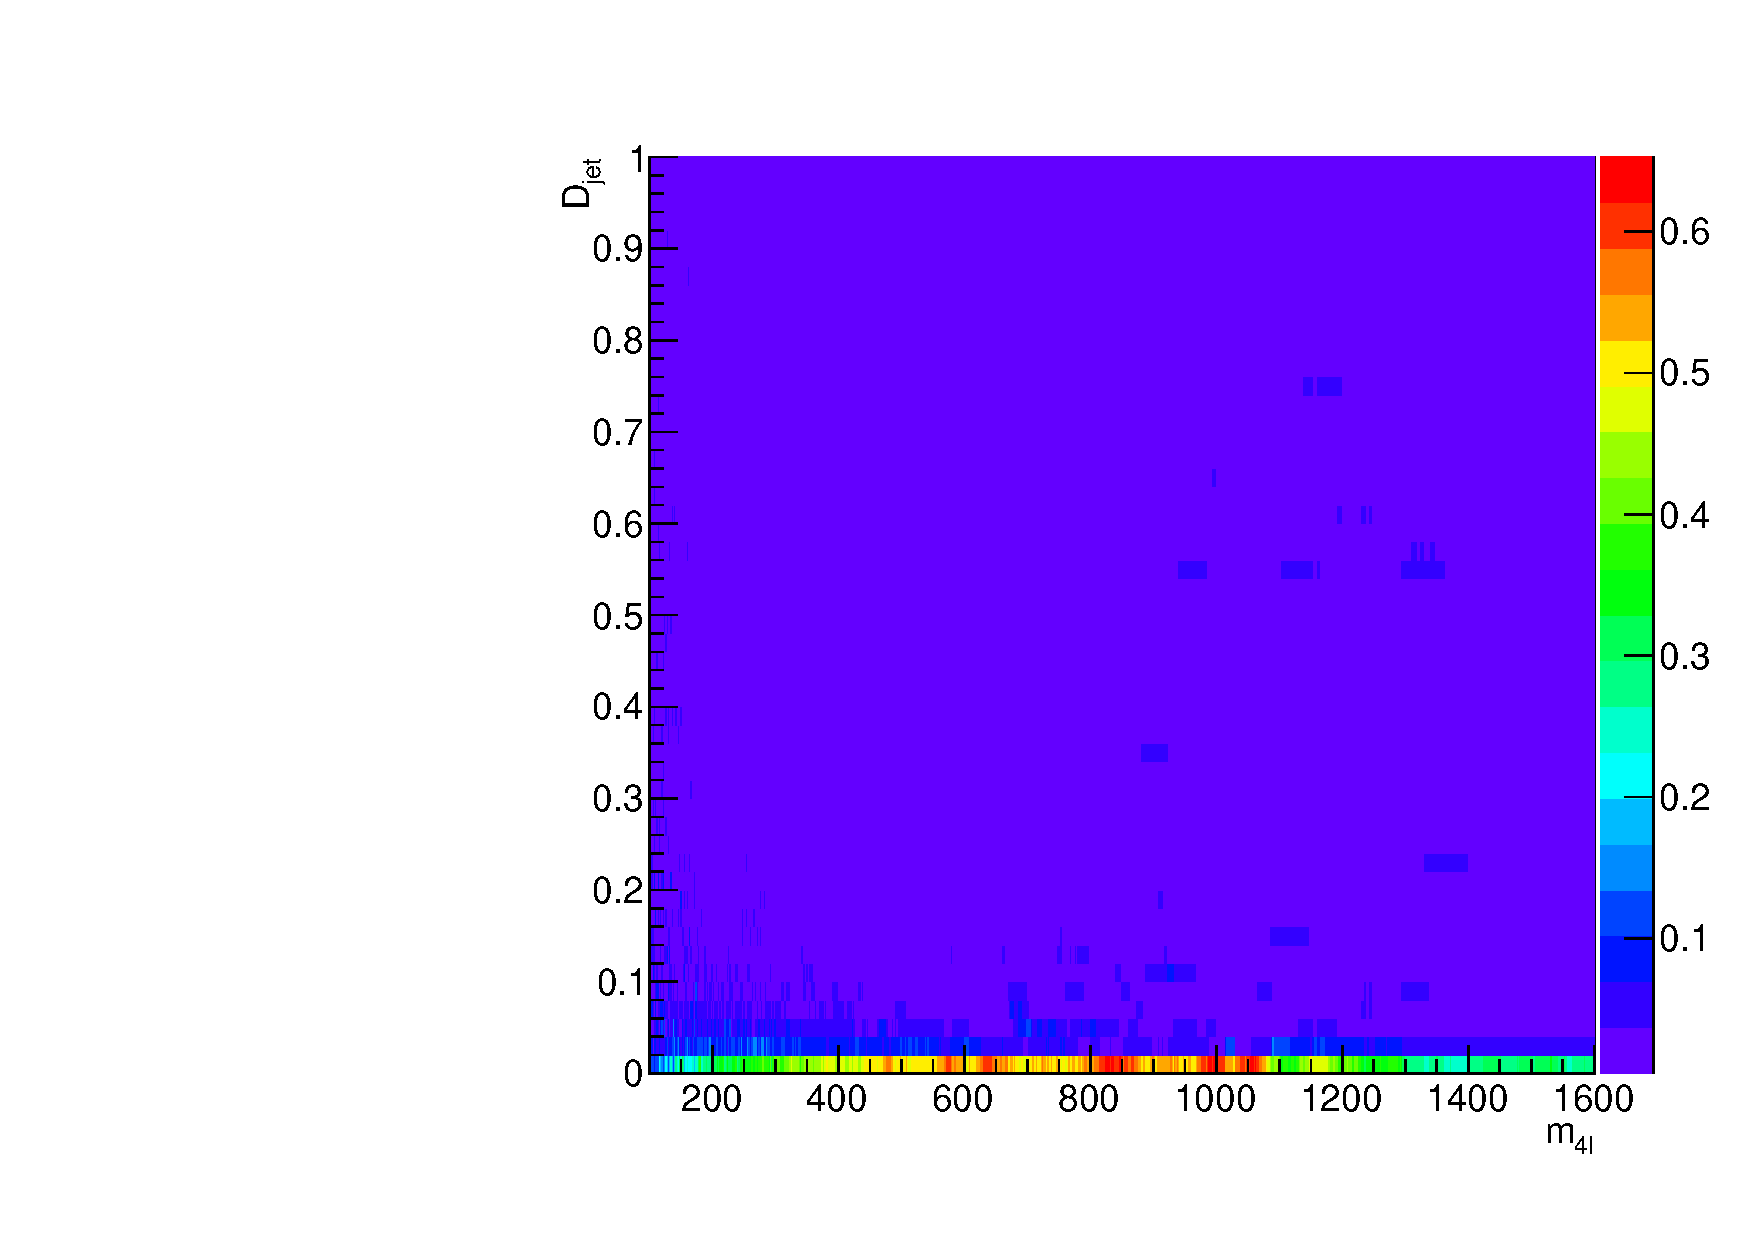
\includegraphics[width=.3\linewidth]{HiggsProperties/figures/qqZZ_Djet_template.pdf}
\caption[Templates of $\mathcal{D}_{\rm{jet}}$ Using vbfMELA]{Templates of $(\mathcal{D}_{\rm{jet}},m_{4\ell})$ using vbfMELA for VBF (left), ggF (middle), and dominant $q\bar{q}\rightarrow 4\ell$ background (right). These templates replace those seen in Fig.~\ref{fig:FisherTemplates} and described in Sec.~\ref{sec:ZZ4lDjet}.}
\label{fig:vbfMELATemplates}
\end{center}
\end{figure}

For the new $(\mathcal{D}_{\rm{jet}},m_{4\ell})$ templates, the largest shape variations are used from the set of alternate shapes listed in Sec.~\ref{sec:ZZ4lDjet}. Other than the shape systematics applied for the mass shape reweighting, all systematic uncertainties for this high mass analysis are identical to Sec.~\ref{sec:ZZ4lSystematics}. 

This procedure was combined with other $WW$ and $ZZ$ decay states to put limits on the mass of any SM-like heavy Higgs boson or EWS resonance. For the former, a Higgs boson with SM-like couplings was excluded across the full combined search range of $145 < m_{H} < 1000$ $\rm{GeV}$, as seen in Fig.~\ref{fig:HMExclusion}. For any BSM resonance, exclusions will change depending on the values of $C'$ and $\mathcal{B}_{\rm{new}}$ used. As $C'$ becomes arbitrarily small, the number of expected events for a given resonance will tend to zero, so the entire range of possibilities cannot be excluded. As seen in Fig.~\ref{fig:EWSExclusions}, the observed limits on these parameters largely agree with the background only expectations. In sum, from the current data and analysis, the data does not support a high mass Higgs-like resonance in the $WW$ nor the $ZZ$ channels.

\begin{figure}[htbp]
\begin{center}
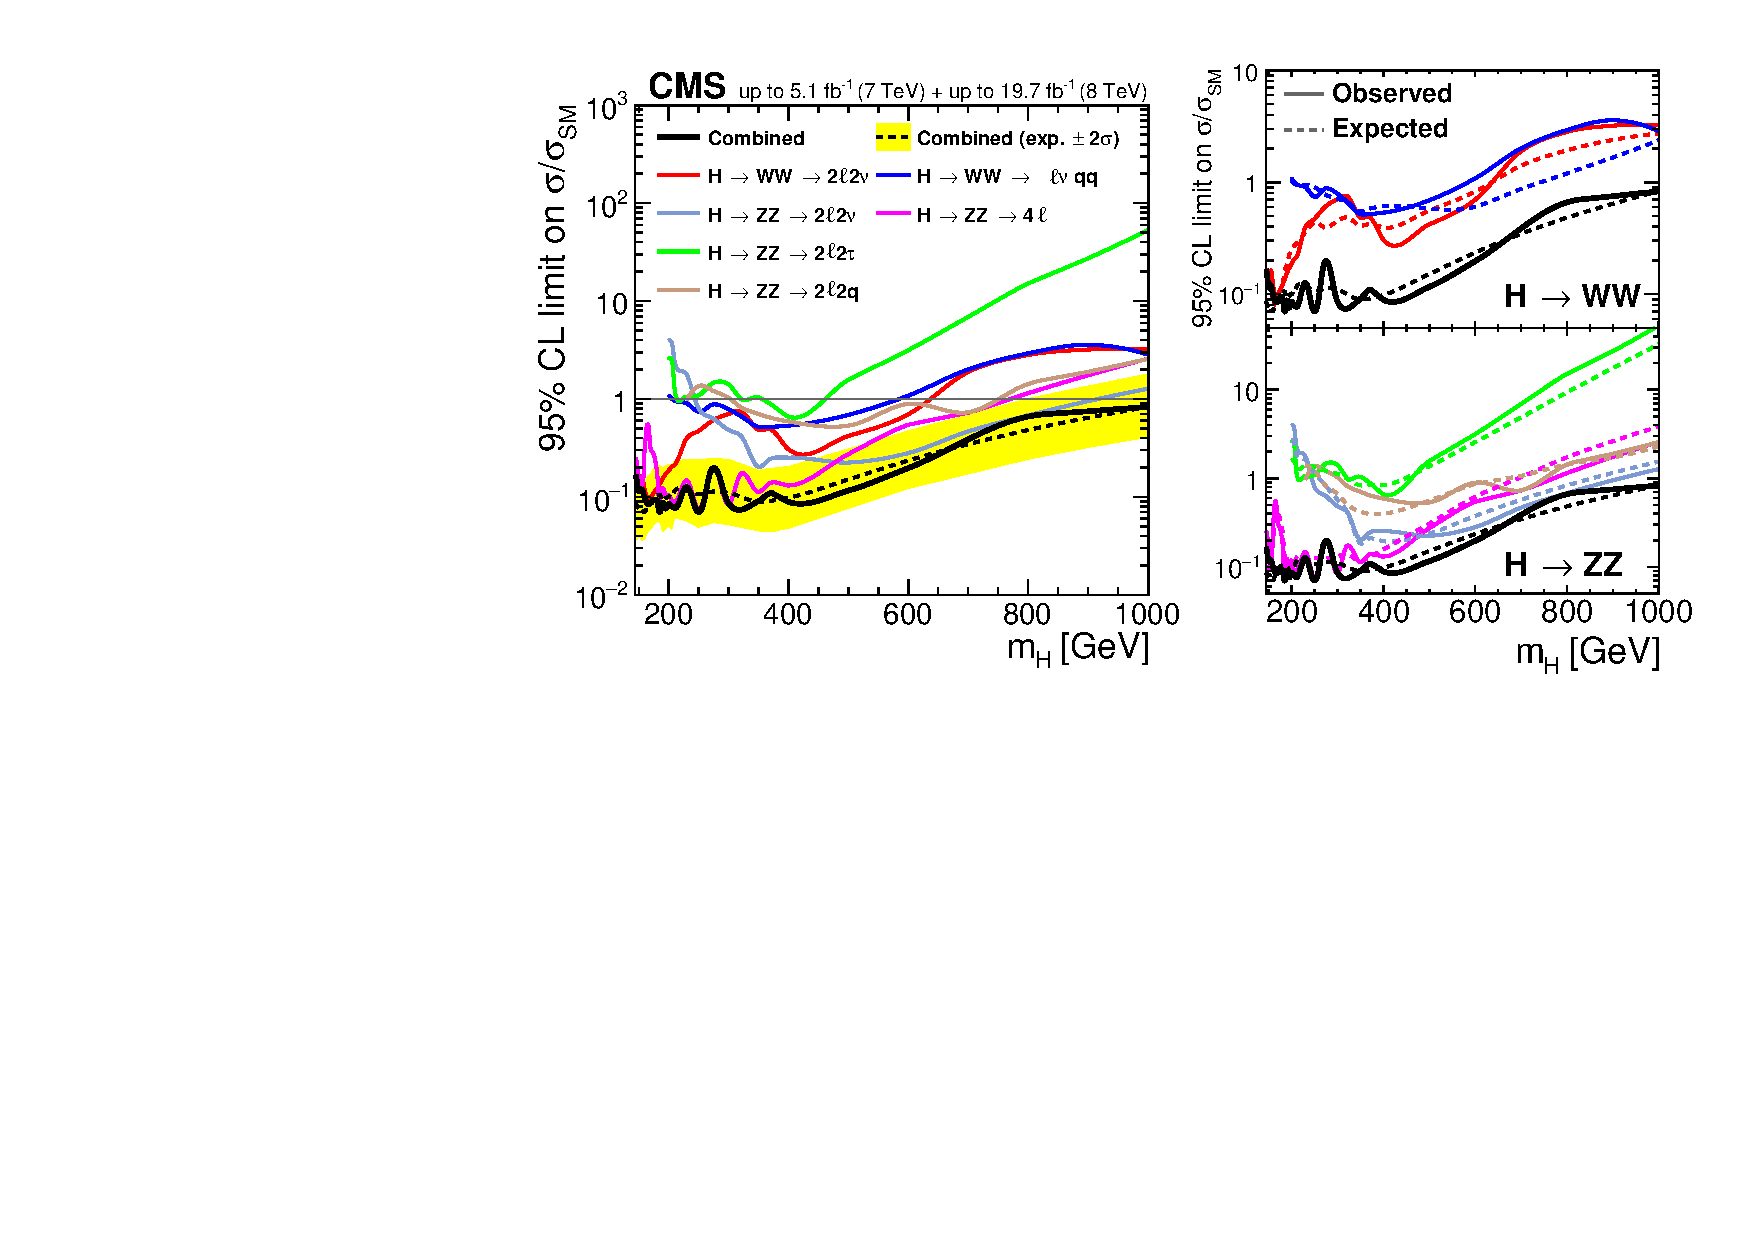
\includegraphics[width=.75\linewidth]{HiggsProperties/figures/combinedSM_def.pdf}
\caption[Combined Expected and Observed Exclusion Limits for High Mass Higgs Search]{Exclusion limits on a Higgs-like high mass resonance in the range $145 < m_{H} < 1000$ $\rm{GeV}$. On left, the combined (black; observed is solid, expected is dashed) and individual limits from all contributing decay channels. For masses below $\lesssim 500$ $\rm{GeV}$, $ZZ\rightarrow 4\ell$ is the most sensitive channel while $ZZ\rightarrow 2\ell2\nu$ is the most sensitive at higher masses. On right, the combined and individual contributions for respective $WW$ and $ZZ$ decay modes show no significant excesses, leading to an observed exclusion of the full range.}
\label{fig:HMExclusion}
\end{center}
\end{figure}

\begin{figure}[htbp]
\begin{center}
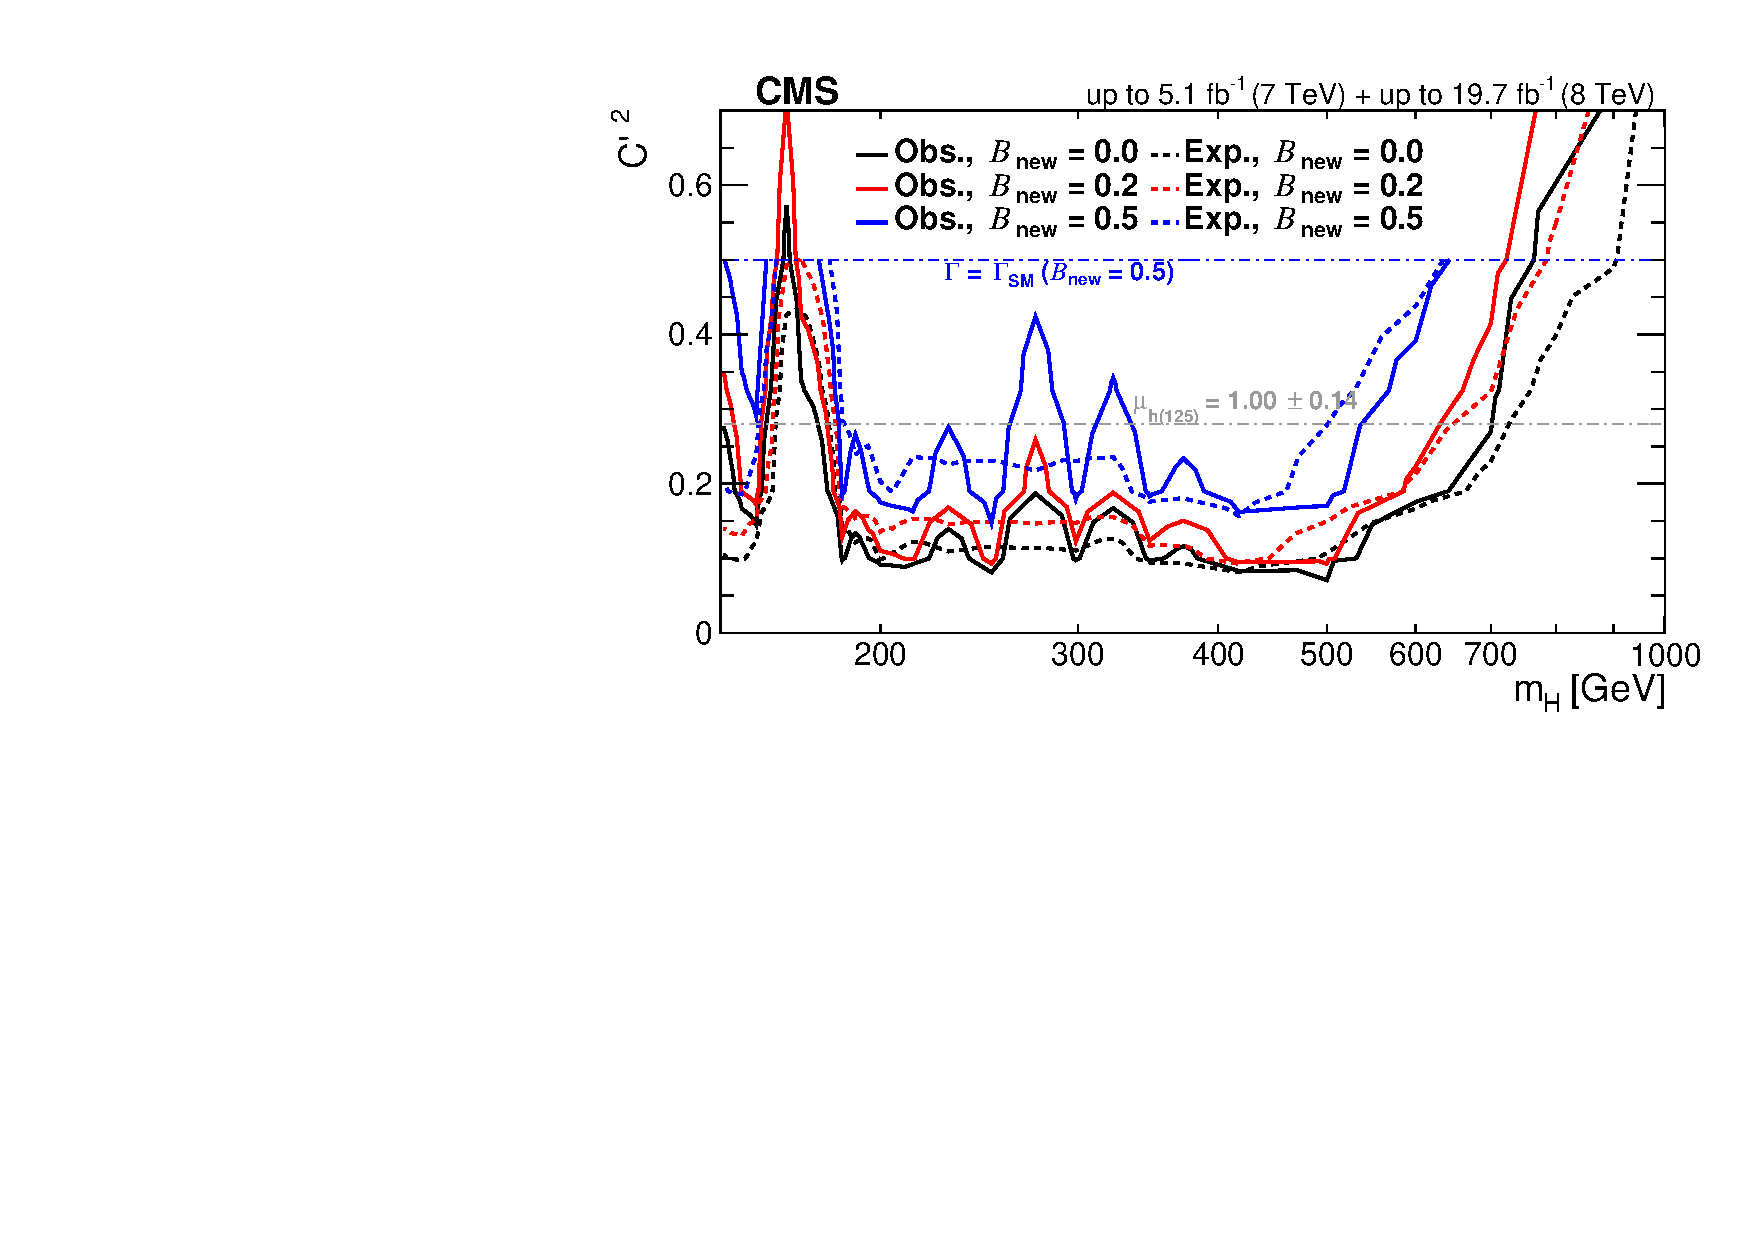
\includegraphics[width=.75\linewidth]{HiggsProperties/figures/combined_BRnewContours.pdf}
\caption[Limits on $C'^2$ for Different Values of $\mathcal{B}_{\rm{new}}$ in the EW Singlet Extension to the Standard Model]{Upper Limits at 95\% CL for $C'^2$ for different values of $\mathcal{B}_{\rm{new}} = 0.0$ (black), 0.2 (red), and 0.5 (blue). For $\mathcal{B}_{\rm{new}} = 0.5$, the dash-dotted blue line at $C'^2 = 0.5$ corresponds to where the width of the high mass resonance is the same as a SM-like Higgs boson - which has been excluded across this range.}
\label{fig:EWSExclusions}
\end{center}
\end{figure}

\section{Higgs Boson Spin-Parity}
\label{sec:SpinParity}

Based on the calculations from Sec.~\ref{sec:HVVDecay}, we utilized the decay kinematics of the $4\ell$ state to separate the SM Higgs boson signal from the dominant $q\bar{q}\rightarrow 4\ell$ background. When searching for the Higgs, this was ideal for discovery. However, now that we have a Higgs boson, what can we say about its spin-parity? It turns out that we can use similar techniques to separate the SM Higgs from different BSM hypotheses and even make measurements as to how tightly this Higgs boson agrees with the Standard Model expectations.

Using the same MELA methods and decay angular distributions, we modify the statistical analysis of Sec.~\ref{sec:ZZ4lAnalysis} by building new discriminants tuned to separate the SM Higgs production from alternative spin-parity models. The LO matrix elements for different spin-parity states are produced using JHUGen while background matrix elements are still generated using {\tt MCFM}. Both are implemented in the MELA package \cite{Chatrchyan:2012ufa,Gao:2010qx,Bolognesi:2012mm,Anderson:2013afp}. Performance of the MELA package was confirmed using the MEKD package \cite{Avery:2012um}, based on {\tt MadGraph}, {\tt FeynRules} \cite{Christensen:2008py}, and analytical parameterizations \cite{Chen:2012jy,Chen:2014pia,Chen:2014gka}. Dedicated MC samples for each alternative spin-parity state were produced using JHUGen. Observed kinematic distributions in data and expected distributions from MC simulations are seen in Fig.~\ref{fig:SPKinDistributions}. A list of alternative spin-parity states that were considered are found in Table~\ref{tbl:JPStates}.

\begin{figure}[htbp]
\begin{center}
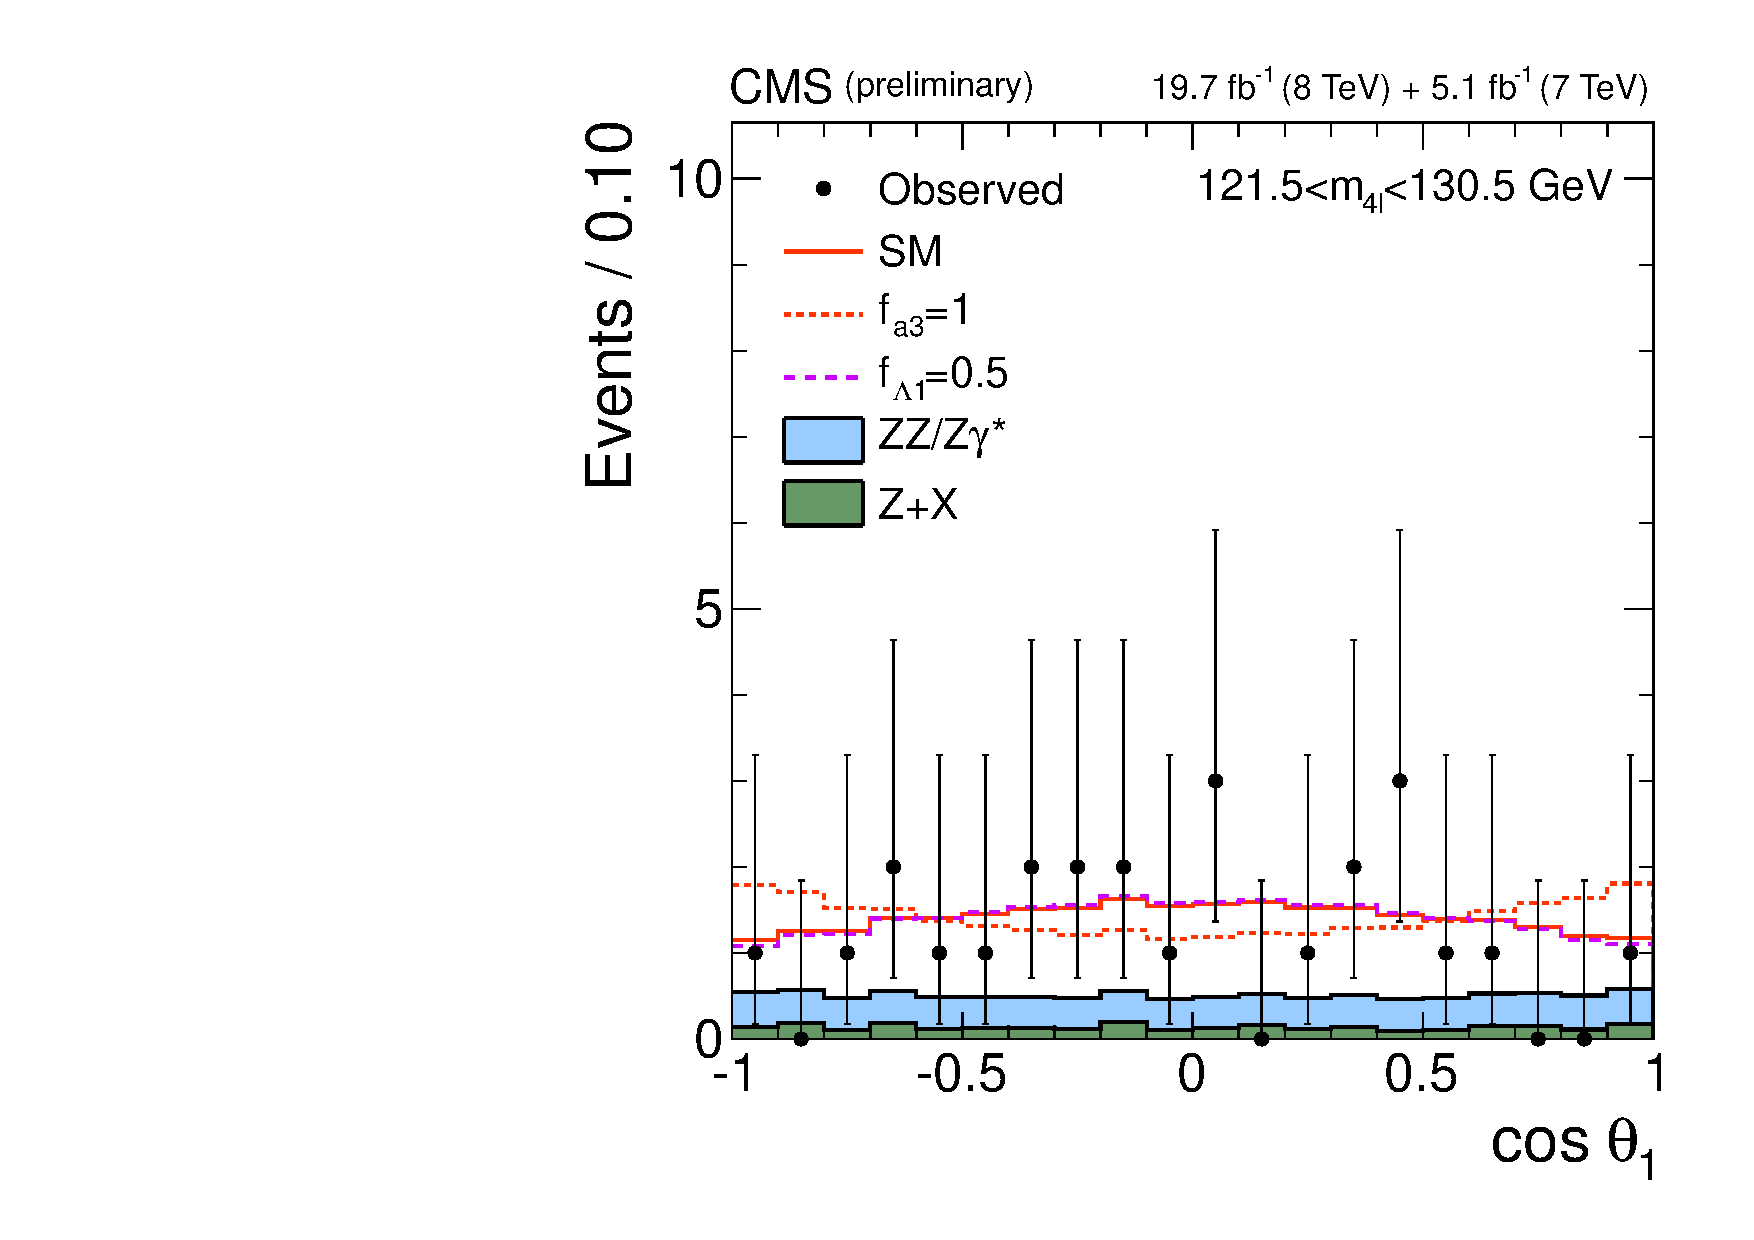
\includegraphics[width=.3\linewidth]{HiggsProperties/figures/cCompare_DataMC_AllTeV_helcosthetaZ1_SignalEnriched.pdf}
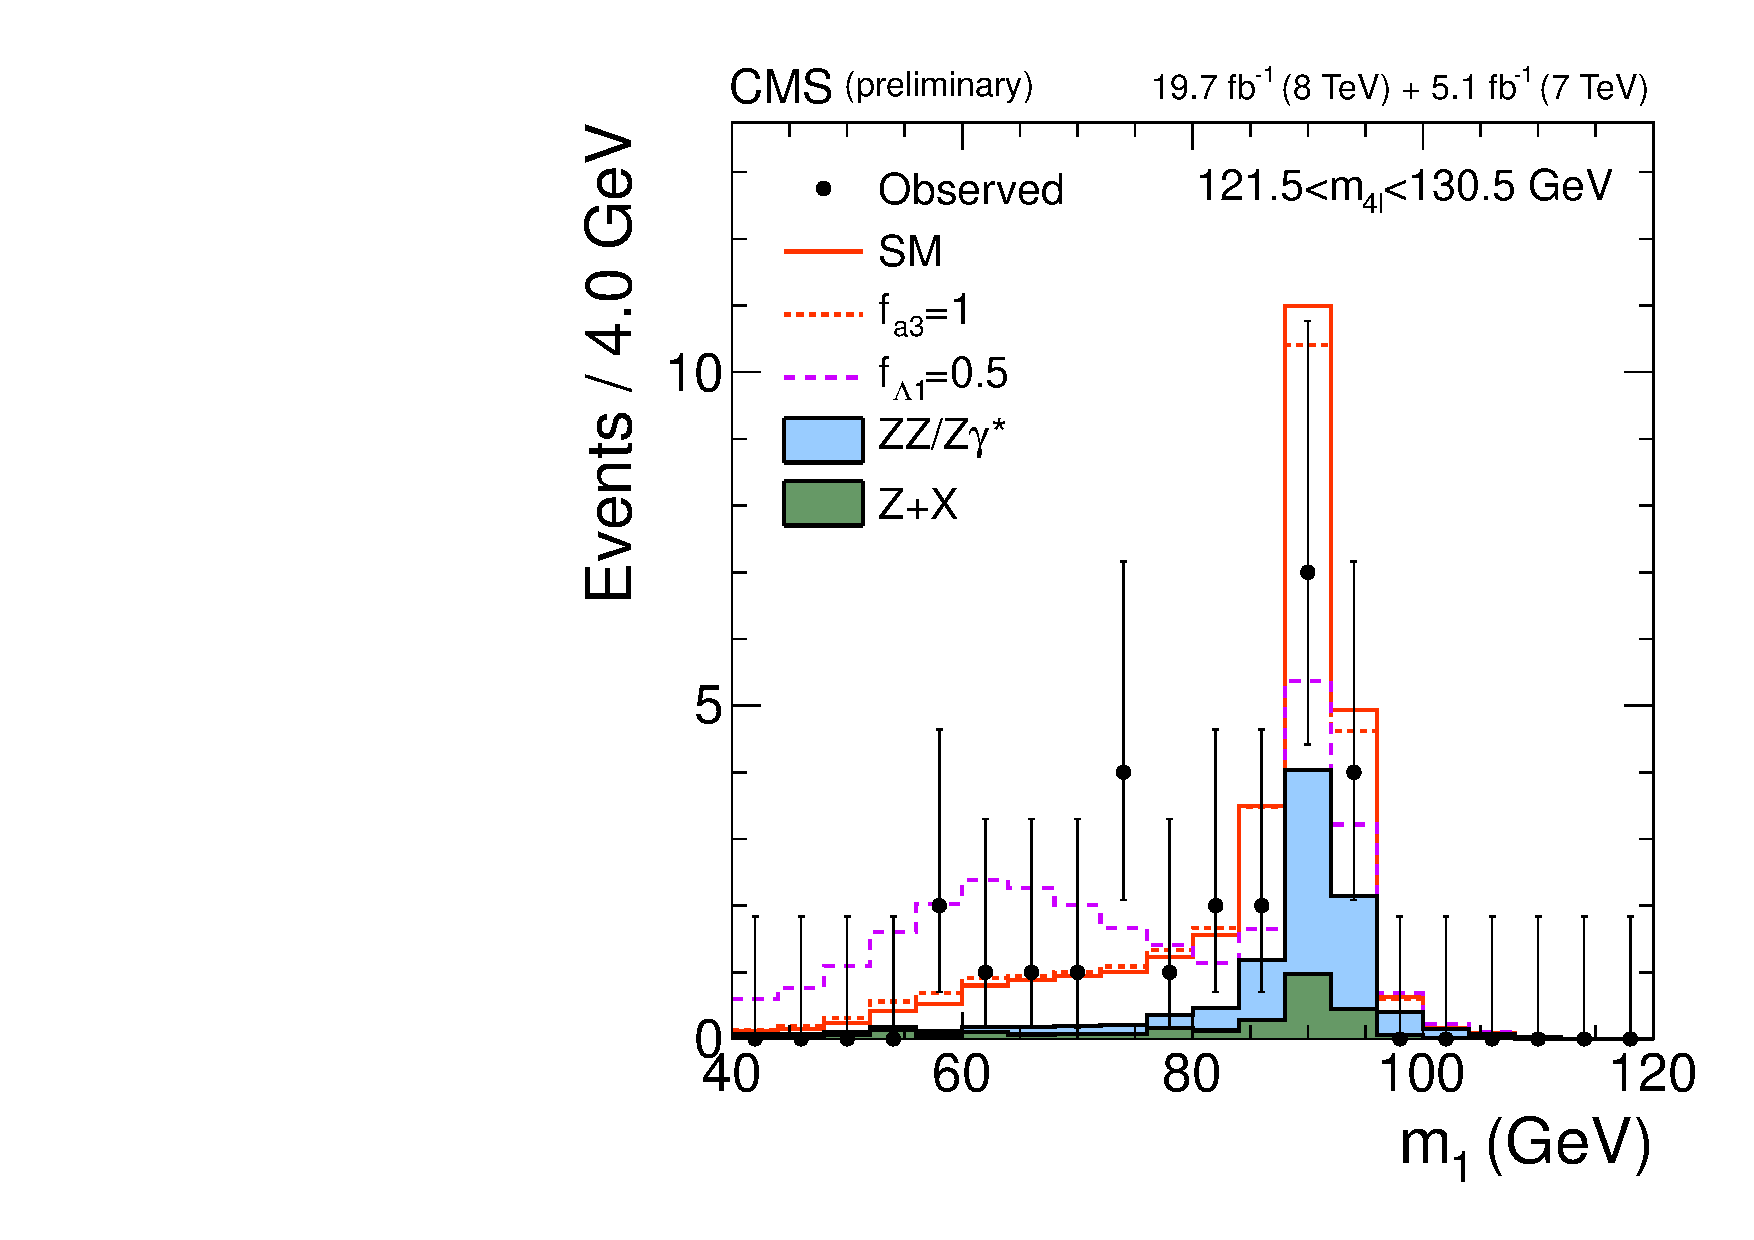
\includegraphics[width=.3\linewidth]{HiggsProperties/figures/cCompare_DataMC_AllTeV_Z1Mass_SignalEnriched.pdf}
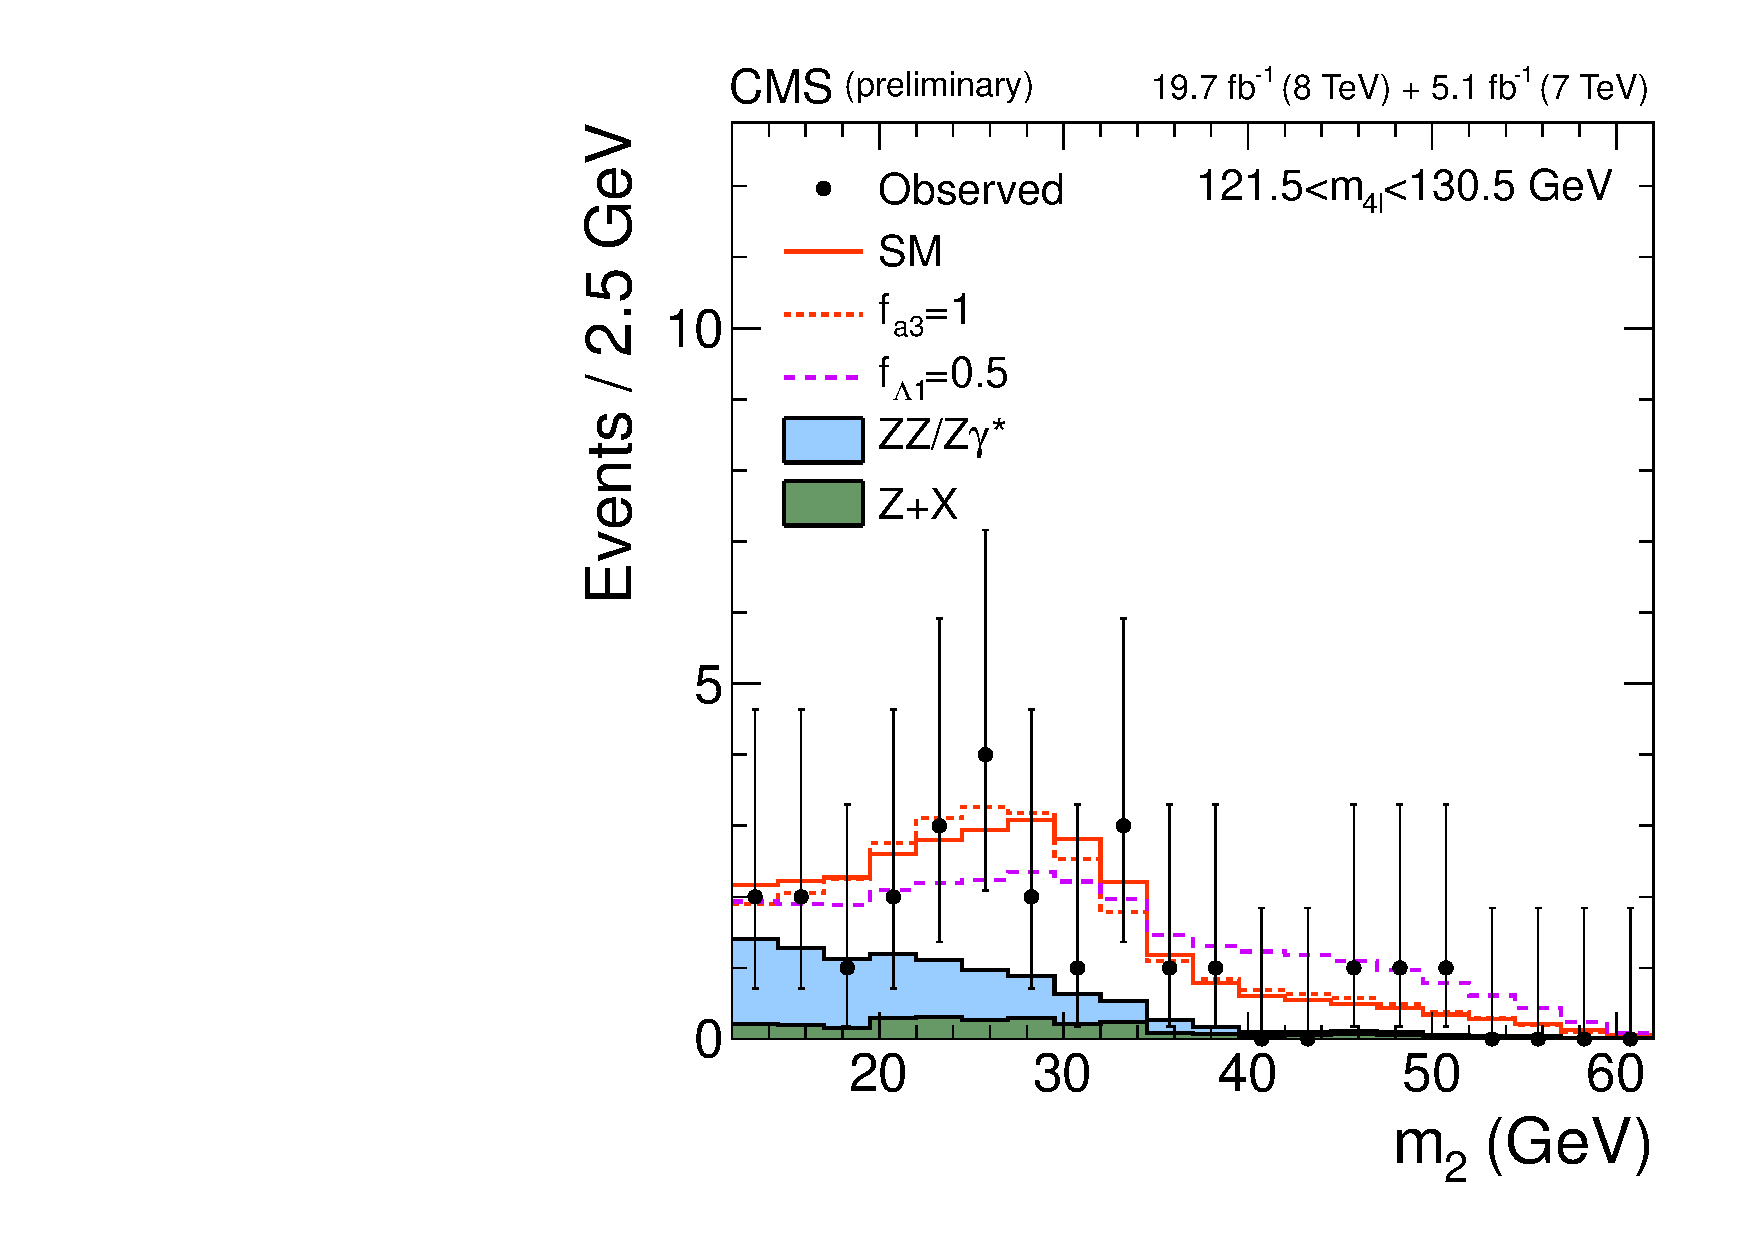
\includegraphics[width=.3\linewidth]{HiggsProperties/figures/cCompare_DataMC_AllTeV_Z2Mass_SignalEnriched.pdf}
\caption[Kinematic Distributions for SM and Alternative Spin-Parity States near $125.6$ $\rm{GeV}$ Resonance]{Distributions of $\cos\theta_1$, $m_{Z1}$, and $m_{Z2}$ for $121.5<m_{4\ell}<130.5$ $\rm{GeV}$. SM Higgs boson (solid red) is compared to a pure-pseudoscalar (dotted red) and $f_{\Lambda 1}=0.5$ (dashed magenta) expectations. SM Background distributions for irreducible $ZZ$ (blue) and reducible $Z+X$ (green) also shown.}
\label{fig:SPKinDistributions}
\end{center}
\end{figure}

\begin{table}[htbp]
\begin{center}
\begin{tabular}{lcclcclccl}
\hline
\hline
\multicolumn{2}{c}{Spin-0} & \multicolumn{2}{c}{Spin-1} & \multicolumn{2}{c}{Spin-2} \\
\hline
$J^P$ & Description & $J^P$ & Description & $J^P$ & Description \\
\hline
$0^+$ & SM Higgs & $1^+$ & Exotic vector & $2_b^+$ & KK Graviton \\
$0^-$ & Pseudoscalar & $1^-$ & Exotic pseudovector & $2_h^+$ & BSM tensor \\
$0_h^+$ & BSM Scalar & & & $2_h^-$ & BSM pseudotensor \\
\hline
\end{tabular}
\caption[List of Alternative Spin-Parity States for $125.6$ $\rm{GeV}$ Resonance]{Sample list of alternative models used in the spin-parity analysis. For spin-0, if the observed boson is close to the Standard Model expectations, limits can be set on the fractional components of these states, see Eqn.~\ref{eqn:fai}. Spin-1 and 2 states were also examined for production dependence. Additional spin-2 states were tested.}
\label{tbl:JPStates}
\end{center}
\end{table}

There are five potentially interesting probabilities to be used:
\begin{align}
& {\mathcal{P}}_{\rm SM} \equiv {\mathcal{P}}^{\rm kin}_{\rm SM} (\vec\Omega, m_1, m_2|m_{4\ell}) \times {\mathcal{P}}^{\rm mass}_{\rm sig} (m_{4\ell}|m_H) \nonumber \\
& {\mathcal{P}}_{\rm J^P} \equiv {\mathcal{P}}^{\rm kin}_{\rm J^P} (\vec\Omega, m_1, m_2|m_{4\ell}) \times {\mathcal{P}}^{\rm mass}_{\rm sig} (m_{4\ell}|m_H) \nonumber \\
& {\mathcal{P}}^{\rm kin}_{\rm interf} \equiv \left({\mathcal{P}}^{\rm kin}_{\rm SM + J^P}(\vec\Omega, m_1, m_2|m_{4\ell}) - g_{J^P}{\mathcal{P}}^{\rm kin}_{\rm J^P}(\vec\Omega, m_1, m_2|m_{4\ell}) - {\mathcal{P}}^{\rm kin}_{\rm SM}(\vec\Omega, m_1, m_2|m_{4\ell}
) \right) \nonumber \\
& {\mathcal{P}}^{\rm kin}_{\rm interf \perp} \equiv \left({\mathcal{P}}^{\rm kin}_{\rm SM + J^P \perp}(\vec\Omega, m_1, m_2|m_{4\ell}) - g_{J^P}{\mathcal{P}}^{\rm kin}_{\rm J^P}(\vec\Omega, m_1, m_2|m_{4\ell}) - {\mathcal{P}}^{\rm kin}_{\rm SM}(\vec\Omega, m_1, m
_2|m_{4\ell}) \right) \nonumber \\
& {\mathcal{P}}_{q\bar{q}ZZ} \equiv {\mathcal{P}}^{\rm kin}_{q\bar{q}ZZ} (\vec\Omega, m_1, m_2|m_{4\ell}) \times {\mathcal{P}}^{\rm mass}_{q\bar{q}ZZ} (m_{4\ell}) \nonumber
\end{align}
where the superscript ``kin" implies that the probability is computed from matrix elements that use the decay kinematics and the superscript ``mass" utilizes $4\ell$ mass parameterizations to determine the probability that an event of that signal or background exists at a given $4\ell$ mass. ${\mathcal{P}}_{\rm SM}$ and ${\mathcal{P}}_{q\bar{q}ZZ}$ refer to the probabilities associated with the SM Higgs and $q\bar{q}ZZ$ backgrounds respectively and are identical to what was used in Sec.~\ref{sec:ZZ4lKD}. To discriminate between other pure models, ${\mathcal{P}}_{\rm J^P}$ refers to the probability associated with a particular spin-parity state ($J^P$, $J$ referring to the spin and $P$ signifying whether a state is P-even [+] or P-odd [-]). Lastly, for mixed spin-parity states, there will be interference between the two states which necessitates the remaining two interference probabilities\footnote{There are two unfamiliar terms in these interference probabilities: ${\mathcal{P}}^{\rm kin}_{\rm SM + J^P}$ or ${\mathcal{P}}^{\rm kin}_{\rm SM + J^P \perp}$ and $g_{J^P}$. The probability term comes from a 50\%-50\% mix between the SM and another $J^P$ state. $g_{J^P}$ is a correction factor.}.

With these probabilities, we again build discriminants:
\begin{align}
& {\mathcal{D}}_{\rm bkg} = \frac{{\mathcal{P}}^{\rm }_{\rm SM} }{{\mathcal{P}}^{\rm }_{\rm SM} +c\times{\mathcal{P}}^{\rm }_{\rm bkg} }=
\left[1+c(m_{4\ell})\times\frac{{\mathcal{P}}^{\rm kin}_{\rm bkg} (m_1, m_2, \vec\Omega | m_{4\ell})\times {\mathcal{P}}^{\rm mass}_{\rm bkg} (m_{4\ell})  }
{{\mathcal{P}}^{\rm kin}_{\rm SM} (m_1, m_2, \vec\Omega | m_{4\ell}) \times {\mathcal{P}}^{\rm mass}_{\rm sig} (m_{4\ell}|m_H) } \right]^{-1} \nonumber \\
& {\mathcal{D}}^{\rm kin}_{J^P} = \frac{{\mathcal{P}}^{\rm kin}_{\rm SM} }{{\mathcal{P}}^{\rm kin}_{\rm SM} +c_{J^P}\times{\mathcal{P}}^{\rm kin}_{J^P} }=
\left[1+c_{J^P}\times\frac{{\mathcal{P}}^{\rm kin}_{J^P} (m_1, m_2, \vec\Omega | m_{4\ell}) }
{{\mathcal{P}}^{\rm kin}_{\rm SM} (m_1, m_2, \vec\Omega | m_{4\ell}) } \right]^{-1} \nonumber \\
& {\mathcal{D}}_{\rm Interf} = \frac{ \left({\mathcal{P}}^{\rm kin}_{\rm SM + J^P} - g_{J^P}{\mathcal{P}}^{\rm kin}_{\rm J^P} - {\mathcal{P}}^{\rm kin}_{\rm SM}\right)}{{\mathcal{P}}^{\rm kin}_{\rm SM} +c_{J^P}\times{\mathcal{P}}^{\rm kin}_{J^P} } \nonumber
\end{align}
where ${\mathcal{D}}_{\rm bkg}$ is very similar to ${\mathcal{D}}_{\rm bkg}^{\rm kin}$ used in Sec.~\ref{sec:ZZ4lKD} but the probability for the mass is also included. ${\mathcal{D}}^{\rm kin}_{J^P}$ is calculated for each alternative $J^P$ hypothesis and ${\mathcal{D}}_{\rm Interf}$ accounts for interference between the alternative $J^P$ shape and the SM shape. As with other discriminants, the constants $c_x$ are used to shift the relative normalizations such that the integrated probability below and above 0.5 are equal. These discriminants are used to populate binned templates for the statistical analysis.

The likelihood analysis changes depending on the spin being examined. As the Higgs boson is expected to be spin-0 from the Standard Model, the analysis is built to quantify any anomalous coupling parameters that would indicate a small deviation from the SM. Following the formalism from Sec.~\ref{sec:HVVDecay}, we aim to extract the parameters from the set $\vec{\xi} = (f_{a2}, \phi_{a2}, f_{a3}, \phi_{a3},f_{\Lambda 1}, \phi_{\Lambda 1})$. For $n_{sig}$ signal events and $n_{bkg}$ background events, we find the likelihood for N candidate events to be
\begin{equation}
{{\mathcal{L}}} =  \exp\left( - n_{\rm sig}(\vec{\xi})-n_{\rm bkg}  \right) \prod_i^{N} \left( n^{SM}_{\rm sig} \times{\mathcal{P}}_{\rm sig}(\vec{x}_{i};~\vec{\xi})  +n_{\rm bkg} \times{\mathcal{P}}_{\rm bkg}(\vec{x}_{i}) \right)
\end{equation}
where the probability distribution functions come from the appropriate templates for a particular anomalous coupling measurement. In principle, ${\mathcal{P}}_{\rm sig}$ depends on all values in $\vec{\xi}$, however we reduce our measurements to only be one or two-dimensional\footnote{Measurements were also taken allowing the respective phases of each $f_{i}$. In this sense, each 1D $f_{i}$ measurement can be extended to a 2D measurement and each 2D $f_{i}$ v $f_{j}$ measurement to a 4D measurement.} and fix all other parameters to the SM values. For 1D measurements, ${\mathcal{P}}_{\rm sig}$ becomes
\begin{equation}
\begin{split}
{\mathcal{P}}_{\rm sig}(\vec{x}_i;f_{i},\phi_{i}) &= (1-f_i) \mathcal{P}_{0^+}(\vec{x}_i) + f_{i} \mathcal{P}_{BSM}(\vec{x}_i) \\ &+\sqrt{f_i (1-f_i)}[\mathcal{P}_{\rm interf}(\vec{x}_i)\cos(\phi_i) + \mathcal{P}_{\rm interf \perp}(\vec{x}_i)\sin(\phi_i)]
\end{split}
\end{equation}
For 2D measurements, we have
\begin{equation}
\begin{split}
{\mathcal{P}}_{\rm sig}(\vec{x}_i;f_{i},f_{j}) &= (1-f_i-f_j) \mathcal{P}_{0^+}(\vec{x}_i) + f_{i} \mathcal{P}_{BSM_1}(\vec{x}_i) + f_{j} \mathcal{P}_{BSM_2}(\vec{x}_i)\\ &+\sqrt{f_i (1-f_i-f_j)}[\mathcal{P}_{\rm interf}^{0^+,BSM_1}(\vec{x}_i)\cos(\phi_i) + \mathcal{P}_{\rm interf \perp}^{0^+,BSM_1}(\vec{x}_i)\sin(\phi_i)] \\
& + \sqrt{f_j (1-f_i-f_j)}[\mathcal{P}_{\rm interf}^{0^+,BSM_2}(\vec{x}_i)\cos(\phi_j) + \mathcal{P}_{\rm interf \perp}^{0^+,BSM_2}(\vec{x}_i)\sin(\phi_j)] \\
& + \sqrt{f_if_j}[\mathcal{P}_{\rm interf}^{BSM_1,BSM_2}(\vec{x}_i)\cos(\phi_i-\phi_j) + \mathcal{P}_{\rm interf \perp}^{BSM_1,BSM_2}(\vec{x}_i)\sin(\phi_i - \phi_j)]
\end{split}
\end{equation}
where $f_i,\phi_i$ come from $\vec{\xi}$ and the $BSM_x$ subscript or superscript refers to the relevant spin-0 model(s).

For Spin-1 and Spin-2, we use the log-likelihood test to separate the SM Higgs boson hypothesis from any alternative spin-parity state. Explicitly, we define the test statistic $q = -2 \ln \frac{\mathcal{L}_X}{\mathcal{L}_{0^+}}$ where the likelihoods are for all events, coming from probability distributions either the SM Higgs ($\mathcal{L}_{0^+}$) or the alternative hypothesis ($\mathcal{L}_{X}$). To quantify the separations, we calculate the probability that the alternative hypothesis has $q$ at the median of the SM expectation. For Spin-1, these likelihoods come from 3D probability distributions built from three discriminants, $({\mathcal{D}}_{1^+},{\mathcal{D}}_{1^-},{\mathcal{D}}_{\rm bkg})$. For Spin-2, the distributions are 2D built from $({\mathcal{D}}_{J^P},{\mathcal{D}}_{\rm bkg})$.

The results of this analysis show that the Higgs boson is widely in agreement with the Standard Model expectations of a spin-0 CP-even particle. In Fig.~\ref{fig:Spin1Exclusions}, all combinations of spin-1 states are excluded. In Fig.~\ref{fig:Spin2Exclusions}, all tested spin-2 states are excluded, many beyond $3\sigma$. All observed anomalous fractions agree with the Standard Model expectations ($J^{PC} = 0^{++}$), as seen in Table~\ref{tbl:Spin0Exclusions}. These results, similar to Sec.~\ref{sec:HighMass}, were combined \cite{Khachatryan:2014kca} with the $WW$ decay channel to get the limits on anomalous couplings for the $HVV$ vertex, as seen in Fig.~\ref{fig:Spin0Exclusions_Combined}.

\begin{figure}[htbp]
\begin{center}
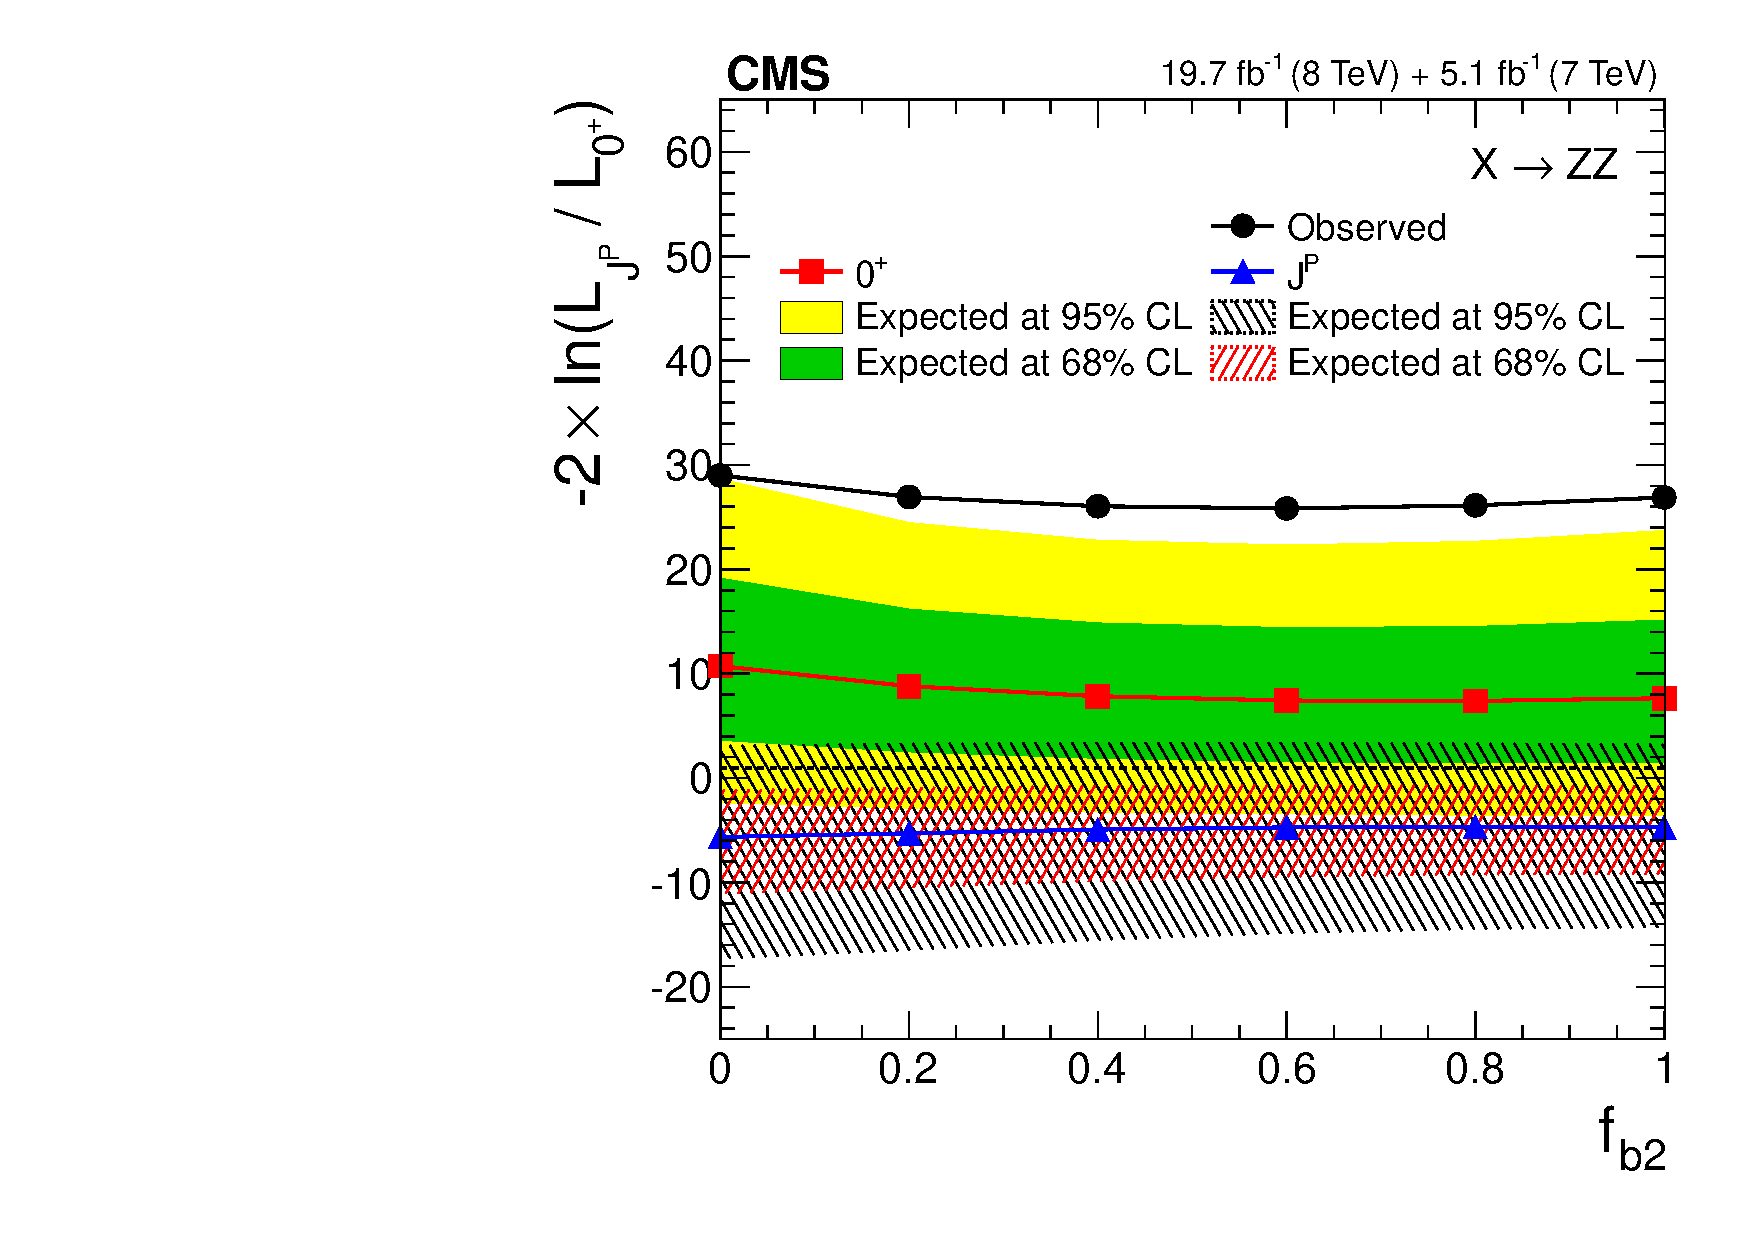
\includegraphics[width=.6\linewidth]{HiggsProperties/figures/summary_PI.pdf}
\caption[Exclusion Limits on Mixed Spin-1 State in $4\ell$ for $125.6$ $\rm{GeV}$ Higgs Boson]{Exclusion limit on the fraction of a mixed spin-1 vector and pseudovector state, $f_{b2}$. Central values of $q = -2 \ln \frac{\mathcal{L}_X}{\mathcal{L}_{0^+}}$ for SM expectations (red squares) and $J^P$ expectations (blue triangles) with $\pm1\sigma$ and $\pm2\sigma$ uncertainty bands. Observed points exclude all values of $f_{b2}$ beyond 95\% CL.}
\label{fig:Spin1Exclusions}
\end{center}
\end{figure}

\begin{figure}[htbp]
\begin{center}
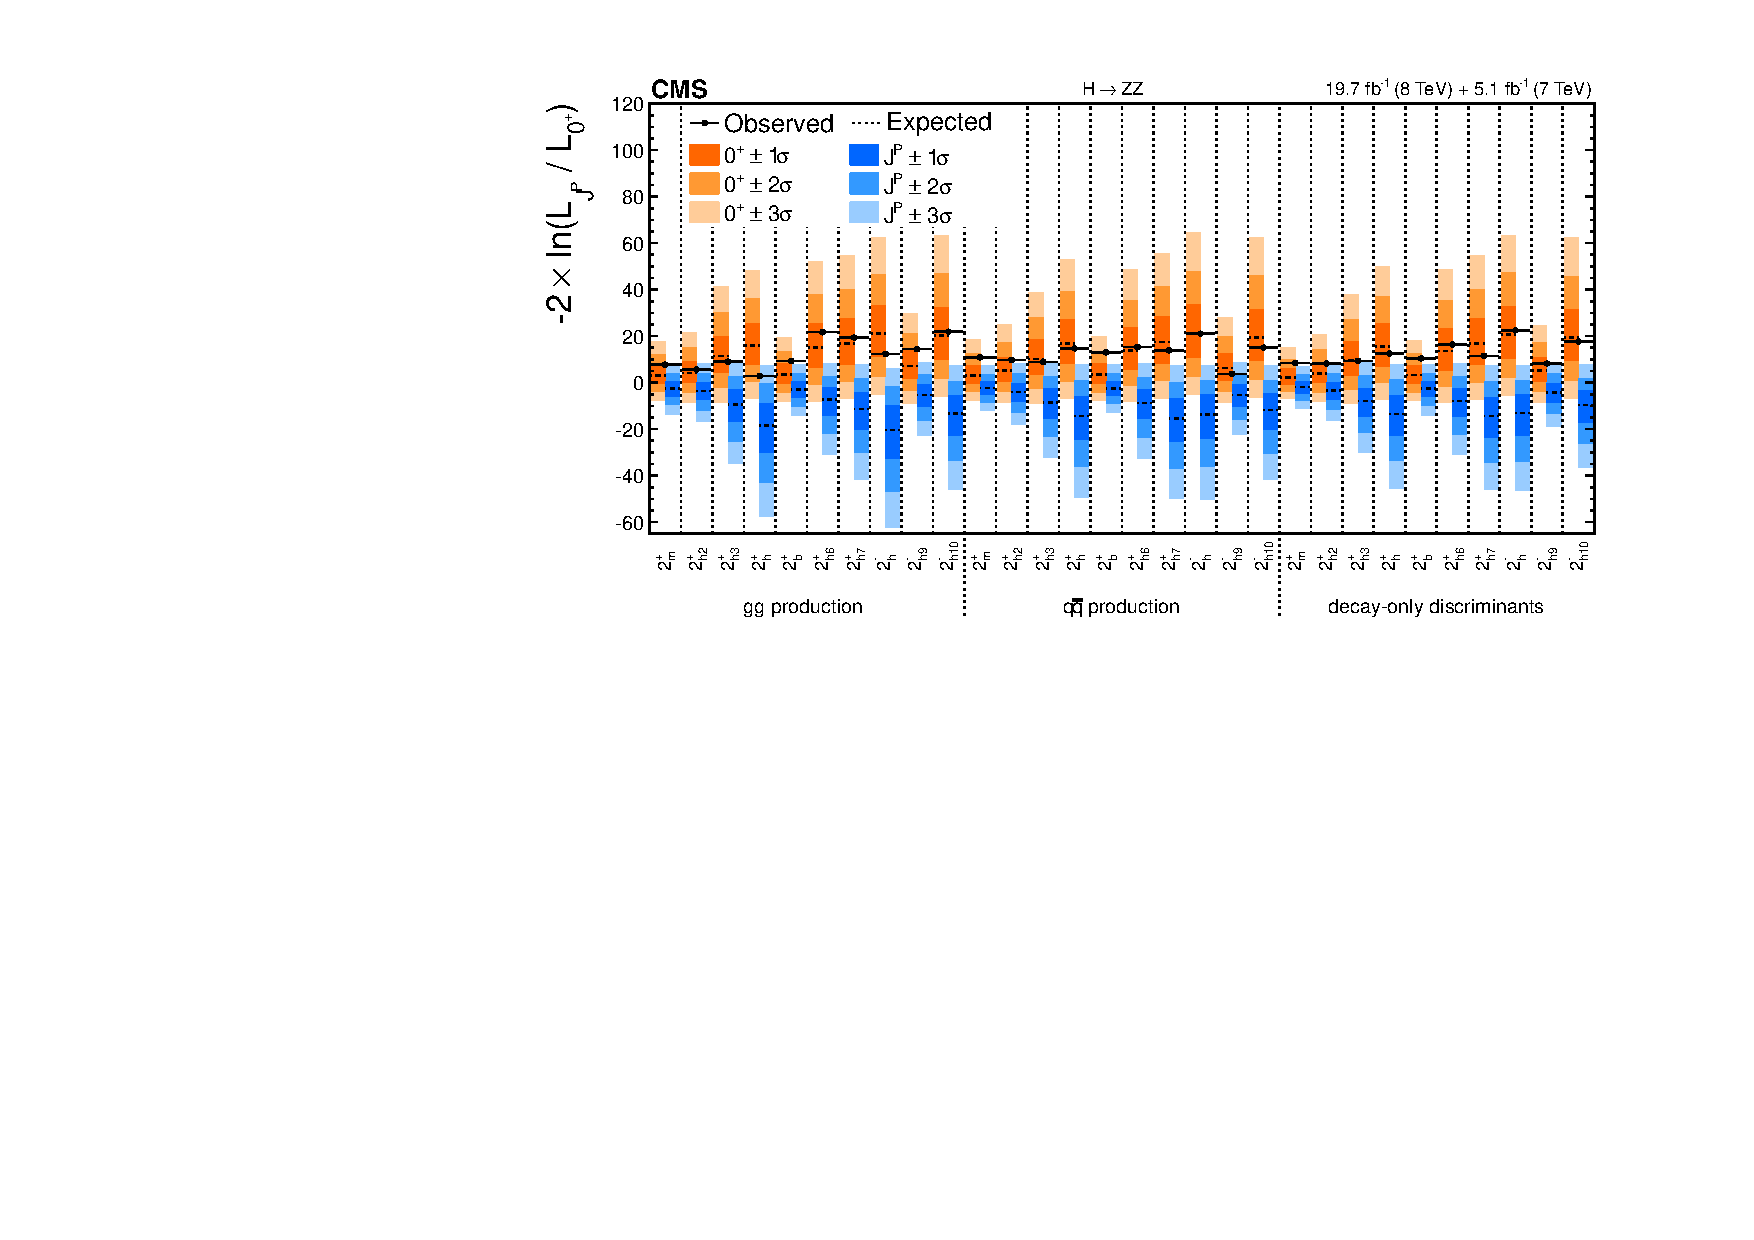
\includegraphics[width=.9\linewidth]{HiggsProperties/figures/JP_SummaryPlot.pdf}
\caption[Summary of Spin-2 Exclusion Limits in $4\ell$ for $125.6$ $\rm{GeV}$ Higgs Boson]{Summary of all tested alternative spin-2 hypotheses in $4\ell$ channel. Orange bands correspond to $\pm1\sigma$, $\pm2\sigma$, and $\pm3\sigma$ uncertainty bands around SM expectations. Blue bands are for each alternative spin-state. Spin-2 particles have different proportions of production methods, so exclusions were set using $gg$-only, $q\bar{q}$-only, and production-independent decay-only discriminants. All tested spin-2 hypotheses are excluded at or above 95\% CL.}
\label{fig:Spin2Exclusions}
\end{center}
\end{figure}

\begin{center}
\begin{table}[htbp]
\begin{tabular}{|c|cc|cc|} 
\hline%--------------------------------------------------------------------------------
\hline%--------------------------------------------------------------------------------
	\multicolumn{5}{|c|}{Allowed 95\%~CL intervals}   \\
\hline%--------------------------------------------------------------------------------
\hline%--------------------------------------------------------------------------------
Parameter ($\phi_{ai}=0$ or $\pi$)                &  \multicolumn{2}{c|}{Observed} &  \multicolumn{2}{c|}{Expected} \\
\hline%--------------------------------------------------------------------------------
$f_{\Lambda1}\cos(\phi_{\Lambda1})$        & \multicolumn{2}{c|}{$ [-0.25,0.37] $}          & \multicolumn{2}{c|}{$ [-1.00,0.27] \cup [0.92,1.00] $}                                            \\
$f_{a2}\cos(\phi_{a2})$         & \multicolumn{2}{c|}{$ [-0.66, -0.57] \cup  [-0.15,1.00]$}     & \multicolumn{2}{c|}{$ [-0.18,1.00]$}            \\
$f_{a3}\cos(\phi_{a3})$         & \multicolumn{2}{c|}{$ [-0.40,0.43] $} & \multicolumn{2}{c|}{$ [-0.70,0.70] $}  \\
\hline%----------------------------------------------------------------------------------
\hline%----------------------------------------------------------------------------------
\end{tabular}
\caption[Summary of Allowed Intervals for Anomalous Spin-0 Couplings in $4\ell$ for $125.6$ $\rm{GeV}$ Higgs Boson]{
Summary of allowed intervals for real values of anomalous spin-0 couplings. $f_i$ values are defined between $[-1.0,1.0]$, by their definitions in Sec.~\ref{sec:HVVVertex}.
}
\label{tbl:Spin0Exclusions}
\end{table}
\end{center}

\begin{figure}[htbp]
\begin{center}
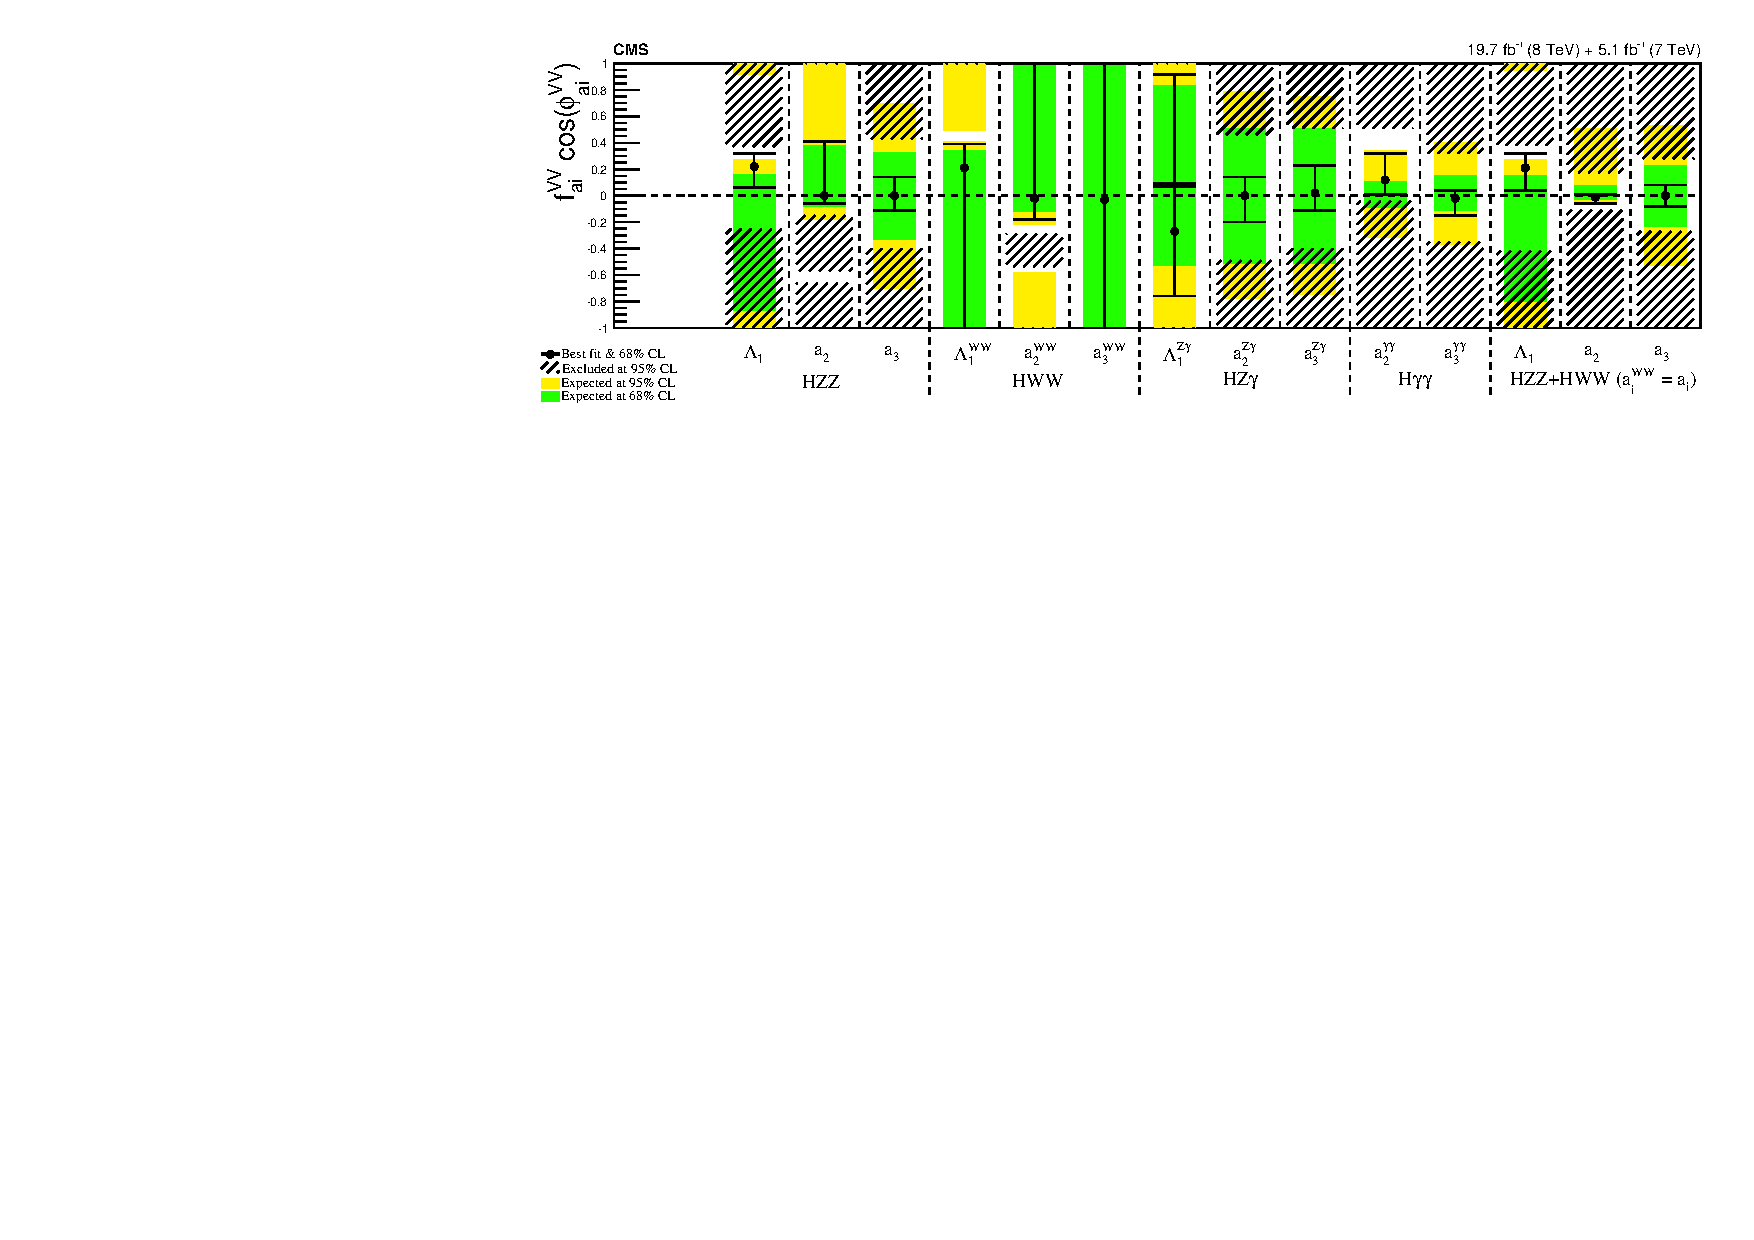
\includegraphics[width=.9\linewidth]{HiggsProperties/figures/Summary_spin0.pdf}
\caption[Summary of Allowed Intervals for Anomalous Spin-0 $HVV$ Couplings for $125.6$ $\rm{GeV}$ Higgs Boson]{Combined limits on real anomalous spin-0 coupling fractions for $HVV$ in CMS. Black points are the best fit values for observations with $\pm1\sigma$ uncertainty. Black hatched regions are excluded at 95\% CL. Green and yellow bands refer to expected regions for SM Higgs boson at 68\% and 95\% CL, respectively.}
\label{fig:Spin0Exclusions_Combined}
\end{center}
\end{figure}

\section{Higgs Boson Width}
\label{sec:Width}

Using the results of Sec.~\ref{sec:ZZ4lResults}, we can reinterpret the mass measurement to put a constraint on the width of the resonance. While the mass measurement assumed a narrow-width resonance, profiling the mass along with the signal strength gives the result in Fig.~\ref{fig:DirectHiggsWidth}. The measured width is $\Gamma_{H} = 0.0^{+1.3}_{-0.0}$ $\rm{GeV}$ with an observed upper limit of $3.4$ $\rm{GeV}$ at the 95\% CL. For $m_H = 125.6$ $\rm{GeV}$, the expected width is $4.15$ $\rm{MeV}$, about 800 times smaller than this limit. Detector resolution places limits on direct measurements of the Higgs boson width and additional statistics will have little practical impact on this limit. This is unfortunate as a potential sign of new physics is a significant deviation from the Standard Model expectations for the width as it would imply that there are decay channels not included in the calculations. Although these measurements are limited by the resolution, there is another method to measure the width.

\begin{figure}[htbp]
\begin{center}
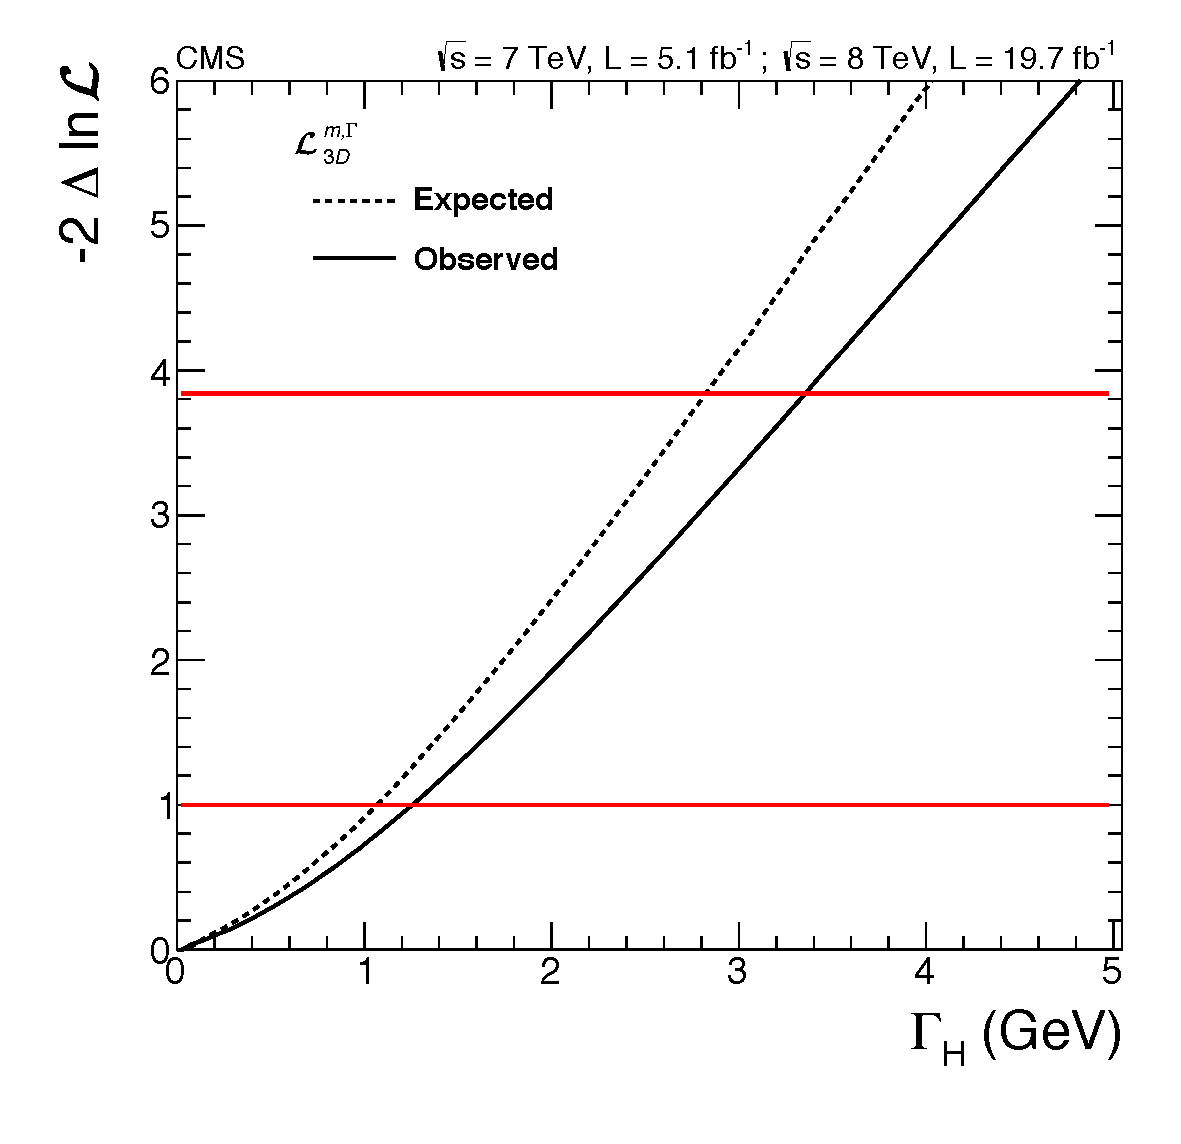
\includegraphics[width=.7\linewidth]{HiggsProperties/figures/width_3D.pdf}
\caption[Direct Measurement of Higgs Width in $4\ell$ Decay Channel]{Likelihood scans of expected (dashed) and observed (solid) widths obtained using 3D fit for mass measurement. Horizontal lines correspond to 68\% and 95\% CL upper limits.}
\label{fig:DirectHiggsWidth}
\end{center}
\end{figure}

\subsection{Finding the Width in the Off-Shell Region}
\label{sec:OffShellPheno}

As argued in Sec.~\ref{sec:ZZ4lMassShape} and Sec.~\ref{sec:HighMass}, for Higgs boson searches where $m_H \lesssim 400$ $\rm{GeV}$, the narrow-width approximation can be used to model the behavior near the on-shell peak. However, this is approximation is not universally valid. For $H\rightarrow VV$ decays, there will be a substantial off-shell enhancement in the region $m_{VV} > 2\times m_{V}$ due to the $2\times m_{V}$ threshold\footnote{Recall the possible decay channels in Sec.~\ref{sec:HiggsDecay}, specifically the branching ratio plots of Fig.~\ref{fig:HXSWGDecay}. After passing the $2\times m_{V}$ threshold, bosonic decays become much more likely. This leads to an off-shell enhancement for $H\rightarrow VV$ decays.} and a further enhancement at the $2\times m_{t}$ threshold\footnote{$gg\rightarrow H$ production requires a fermionic loop, dominated by the contribution from the top quark. When $m_H > 2\times m_{t}$, there will be an additional enhancement, as expected via the branching ratios of Fig.~\ref{fig:HXSWGDecay}.}; nearly 10\% of the total cross section for $H\rightarrow ZZ$ will be above $2\times m_{Z}$ \cite{Kauer:2012hd,Kauer:1305.2092}. When applying the kinematic selection of the $4\ell$ channel, this increases to about 20\% of the total cross section. 

By measuring the off-shell contribution simultaneously with the on-shell, we can make a direct measurement of the total width of the Higgs boson \cite{CaolaMelnikov:1307.4935}. Generally, the differential cross section of the Higgs boson as a function of $m_{4\ell}$ is 
\begin{equation}
\frac{d\sigma_{gg\rightarrow H\rightarrow ZZ\rightarrow 4\ell}}{dm^2_{4\ell}} \sim \sigma_{gg\rightarrow H} \frac{m_{4\ell}^2}{(m_{4\ell}^2-m_{H}^2)^2+m_H^2\Gamma_{H}^2}\frac{\Gamma_{H\rightarrow ZZ \rightarrow 4\ell}(m_{4\ell})}{m_{4\ell}}
\label{eqn:DiffCrossSection}
\end{equation}
where $\sigma_{gg\rightarrow H}$ is the cross section of the Higgs boson produced via gluon-gluon fusion, $\Gamma_{H}$ is the total width of the Higgs boson, and $\Gamma_{H\rightarrow 4\ell}$ is the partial width\footnote{If the total width accounts for all possible decay channels, then the partial width comes only from the branching to a particular decay channel.} of the Higgs boson for the $ZZ\rightarrow 4\ell$ decay channel. The zero width approximation (ZWA) finds the on-shell cross section by integrating over a mass region that spans a number of widths near the peak, covering a narrow $m_{4\ell}$ window:
\begin{equation}
\begin{split}
\sigma_{gg\rightarrow H\rightarrow 4\ell}^{\rm on-shell} &\sim \sigma_{gg\rightarrow H}m_{H}\Gamma_{H\rightarrow 4\ell}(m_{H})\int_{m_H-n\Gamma_H}^{m_H+n\Gamma_H} \frac{1}{\pi}\frac{1}{(m_{4\ell}^2-m_{H}^2)^2 + m_H^2\Gamma_H^2}dm_{4\ell}^2 \\
&\sim \sigma_{gg\rightarrow H}m_{H}\Gamma_{H\rightarrow 4\ell}(m_{H})\frac{1}{m_H\Gamma_H} = \sigma_{gg\rightarrow H}\frac{\Gamma_{H\rightarrow 4\ell}}{\Gamma_H}
\end{split}
\end{equation}
Using an explicit definition\footnote{We know from Sec.~\ref{sec:LHC} that the cross section can be thought of as the likelihood of a certain process occurring. When we look at the total cross section $\sigma_{gg\rightarrow H}$, we can find the cross section just for $gg \rightarrow H \rightarrow ZZ \rightarrow 4\ell$ by multiplying the total cross section by the branching ratio found via the ratio of widths: $\sigma_{gg\rightarrow H \rightarrow ZZ \rightarrow 4\ell} = \sigma_{gg\rightarrow H} \frac{\Gamma_{H \rightarrow 4\ell}}{\Gamma_{H}}$.} of $\sigma_{gg\rightarrow H}\times\Gamma_{H\rightarrow 4l} = \left(\kappa_g\kappa_Z\right)^2(\sigma\cdot BR)_{SM}\Gamma_{H}^{SM}$, with the $\kappa$ notation\footnote{The $\kappa$ notation is used to define the ratios of the measured couplings of particles to the Higgs boson compared to SM expectations, where $\kappa_g = g_{ggH}/g_{ggH}^{SM}$ and $\kappa_Z = g_{HZZ}/g_{HZZ}^{SM}$.} introduced in \cite{Higgs4lLegacy:2013}, we can rewrite the on-shell cross section as
\begin{equation}
\sigma_{gg\rightarrow H\rightarrow 4\ell}^{\rm on-shell} = \frac{\kappa_g^2\kappa_Z^2}{\Gamma_{H}}\Gamma_{H}^{SM}(\sigma\cdot BR)_{SM} \equiv \mu(\sigma\cdot BR)_{SM} 
\label{eqn:DiffCrossSection_OnShell}
\end{equation}
which is ultimately what is measured in the on-shell results previously discussed. There clearly is a degeneracy in this measurement: if the couplings ($\kappa_g^2\kappa_Z^2$) and total width of the Higgs boson ($\Gamma_H$) scale appropriately, $\mu$ will remain unchanged.

This degeneracy can be broken by also looking off-shell. When $m_{4\ell}>2\times m_{Z}$, the $(m_{4\ell}^2-m_{H}^2)^2 \approx m_{4\ell}^4$ term in Eqn.~\ref{eqn:DiffCrossSection} will dominate the denominator. Ultimately, this means that just past the $2\times m_{Z}$ threshold, there will be a plateau in the differential cross section~\cite{Kauer:2012hd,Kauer:1305.2092}, causing an off-shell enhancement in this mass range. Using the high mass approximation, we also find
\begin{equation}
\begin{split}
\frac{d\sigma_{gg\rightarrow H\rightarrow ZZ\rightarrow 4\ell}^{\rm off-shell}}{dm^2_{4\ell}} &\sim \sigma_{gg\rightarrow H} \frac{m_{4\ell}^2}{(m_{4\ell}^2-m_{H}^2)^2+m_H^2\Gamma_{H}^2}\frac{\Gamma_{H\rightarrow 4\ell}(m_{4\ell})}{m_{4\ell}} \\
&\sim \kappa_g^2\kappa_Z^2 \cdot \sigma_{gg\rightarrow H}^{SM} \frac{m_{4\ell}^2}{(m_{4\ell}^2-m_{H}^2)^2}\frac{\Gamma_{H\rightarrow 4\ell}^{SM}(m_{4\ell})}{m_{4\ell}} \\
&\sim \kappa_g^2\kappa_Z^2 \cdot \frac{d\sigma_{gg\rightarrow H\rightarrow ZZ\rightarrow 4\ell}^{{\rm off-shell},SM}}{dm^2_{4\ell}}.
\end{split}
\end{equation}
That is, contrary to the on-shell region, the differential cross section \textit{only} depends on the couplings. If we combine this with the on-shell relation of Eqn.~\ref{eqn:DiffCrossSection_OnShell}, we arrive at a measurement that can provide the total width of the Higgs boson:
\begin{equation}
\frac{d\sigma_{gg\rightarrow H\rightarrow ZZ\rightarrow 4\ell}^{\rm off-shell}}{dm^2_{4\ell}} = \mu r \frac{d\sigma_{gg\rightarrow H\rightarrow ZZ\rightarrow 4\ell}^{{\rm off-shell},SM}}{dm^2_{4\ell}}
\label{eqn:OffShellMeasurement}
\end{equation}
where $r=\Gamma_{H}/\Gamma_{H}^{SM}$. Explicitly, for a given value of $\mu$, a measurement of the off-shell cross-section of $m_{4\ell}$ is equivalent to a direct measurement of the total width.

\subsection{Off-Shell $4\ell$ Analysis}
\label{sec:OffShellAnalysis}

The strategy to examine the width is to combine the on-shell analysis with a similar analysis in the higher mass off-shell region. Largely, the analyses are similar: the same datasets and MC samples (Sec.~\ref{sec:ZZ4lMCandData}) are used with identical selection requirements (Sec.~\ref{sec:ZZ4lSelection}). But, there are two additional complications when looking at high masses, which were already encountered in Sec.~\ref{sec:HighMass}: interference of signal and background with the same initial states and the increased role of VBF production.

For interference, we need to expand Eqn.~\ref{eqn:OffShellMeasurement} to account for the $gg\rightarrow ZZ$ background. As discussed in Sec.~\ref{sec:HighMass}, the interference term will scale as the square root of the signal strength, so Eqn.~\ref{eqn:OffShellMeasurement} becomes:
\begin{equation}
\frac{d\sigma_{gg\rightarrow 4\ell}}{dm_{4\ell}} = \mu r \frac{d\sigma_{gg\rightarrow H \rightarrow 4\ell}}{dm_{4\ell}} + \sqrt{\mu r} \frac{d\sigma_{\rm interference}}{dm_{4\ell}} + \frac{d\sigma_{gg\rightarrow ZZ \rightarrow 4\ell}}{dm_{4\ell}}
\label{eqn:OffShellDiff_ZZ}
\end{equation}
To find the $m_{4\ell}$ shapes needed for each component, samples for $gg\rightarrow 4\ell$ were generated at LO using both {\tt GG2VV 3.1.5} and {\tt MCFM 6.7} with $m_H=125.6$ $\rm{GeV}$. Sample $m_{4\ell}$ shapes generated from {\tt GG2VV} are shown in Fig.~\ref{fig:gg2VVDiffXSec}. Agreement between {\tt GG2VV} and {\tt MCFM} samples can be seen in Fig.~\ref{fig:gg2VVMCFMComparison}.

\begin{figure}[htbp]
\begin{center}
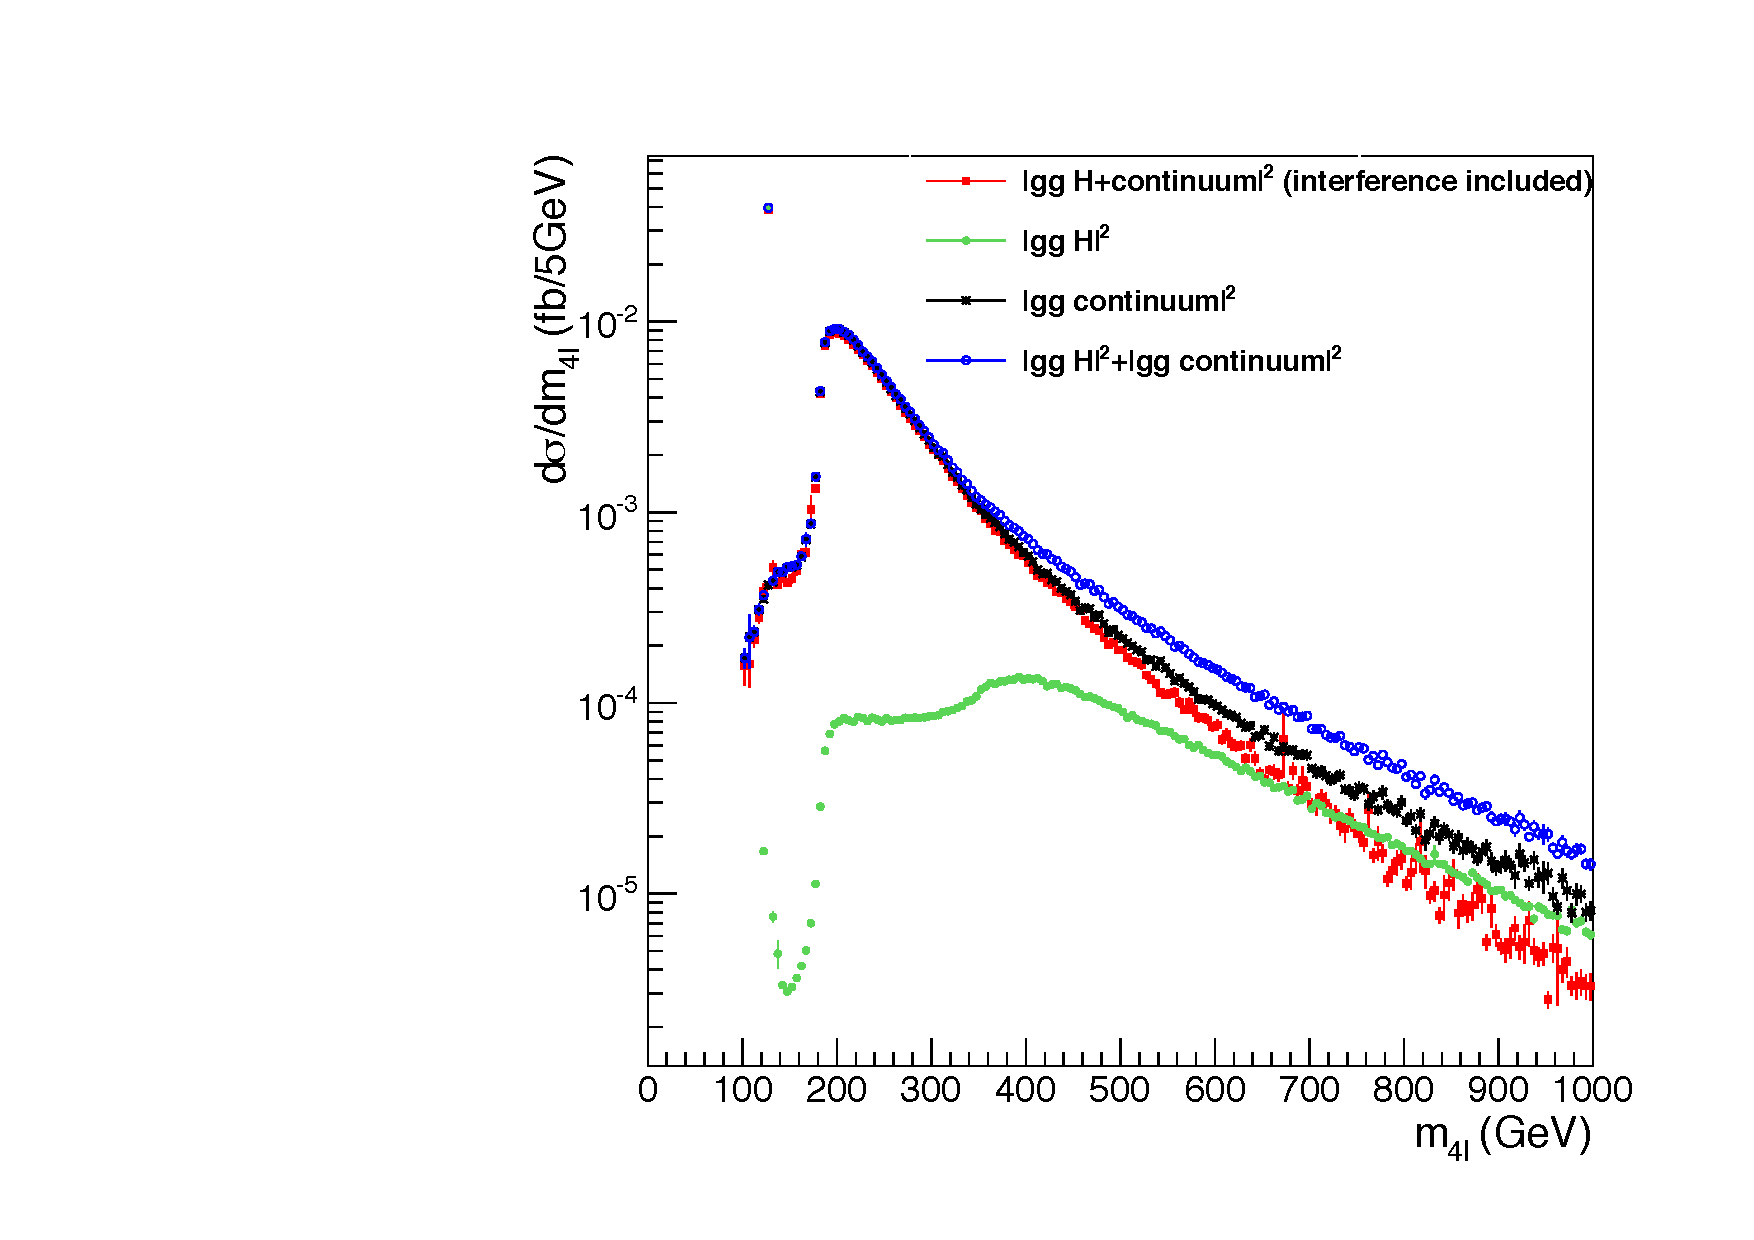
\includegraphics[width=.5\linewidth]{HiggsProperties/figures/gg2VV.pdf}
\caption[Differential Cross Section at LO from gg2VV for Off-shell Region]{Differential cross sections for different processes in $2\ell2\ell'$ final state and 8 $\rm{TeV}$ beam energy found at LO from {\tt GG2VV}. Off-shell signal only (solid green circles) shows enhancement for $m_{4\ell} \gtrsim 2\times m_Z$ with additional enhancement around $2\times m_{t}$. Compared to background only (black crosses) and the unphysical sum of the background and signal (blue open circles), the physical background and signal combination (solid red squares) shows destructive interference.}
\label{fig:gg2VVDiffXSec}
\end{center}
\end{figure}

\begin{figure}[htbp]
\begin{center}
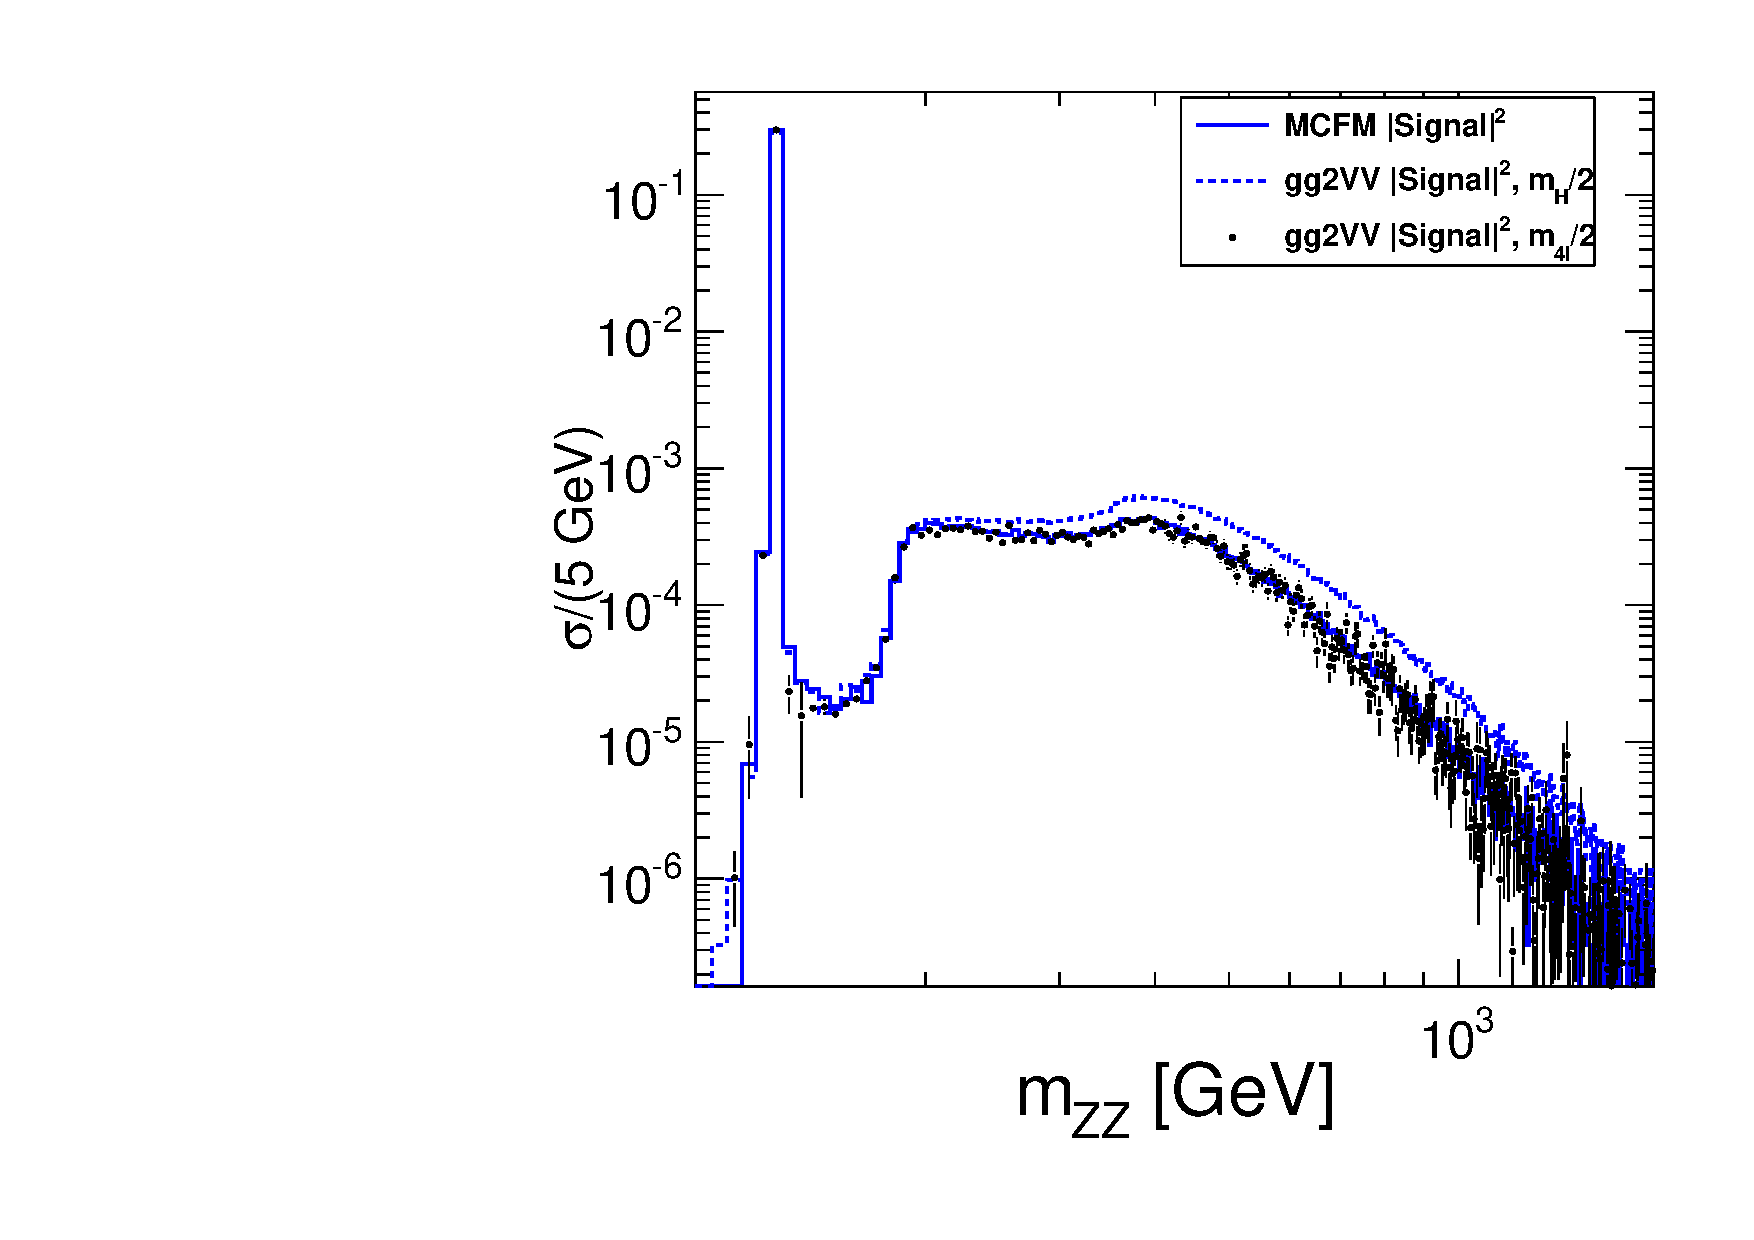
\includegraphics[width=.5\linewidth]{HiggsProperties/figures/gg2VVvsMCFM.pdf}
\caption[Comparison of Off-shell Differential Cross Section between gg2VV and MCFM]{Comparison of off-shell signal only $m_{4\ell}$ distributions between {\tt GG2VV} (blue lines) and {\tt MCFM} (black dots) generators. When both generators use the same running factorization and renormalization scale (solid blue is fixed scale, dashed blue is running scale), the generators show very good agreement in the off-shell region.}
\label{fig:gg2VVMCFMComparison}
\end{center}
\end{figure}

For VBF and VH off-shell production, as was done in Sec.~\ref{sec:HighMass}, {\tt PHANTOM} was used to generate the off-shell samples with the same caveat that signal-only shapes cannot be produced directly so linear combinations of samples with different widths can be used to model the signal and interference contributions. Comparisons of VBF and gluon fusion off-shell processes are shown in right plot of Fig.~\ref{fig:VBFvggF_OffShell}.

\begin{figure}[htbp]
\begin{center}
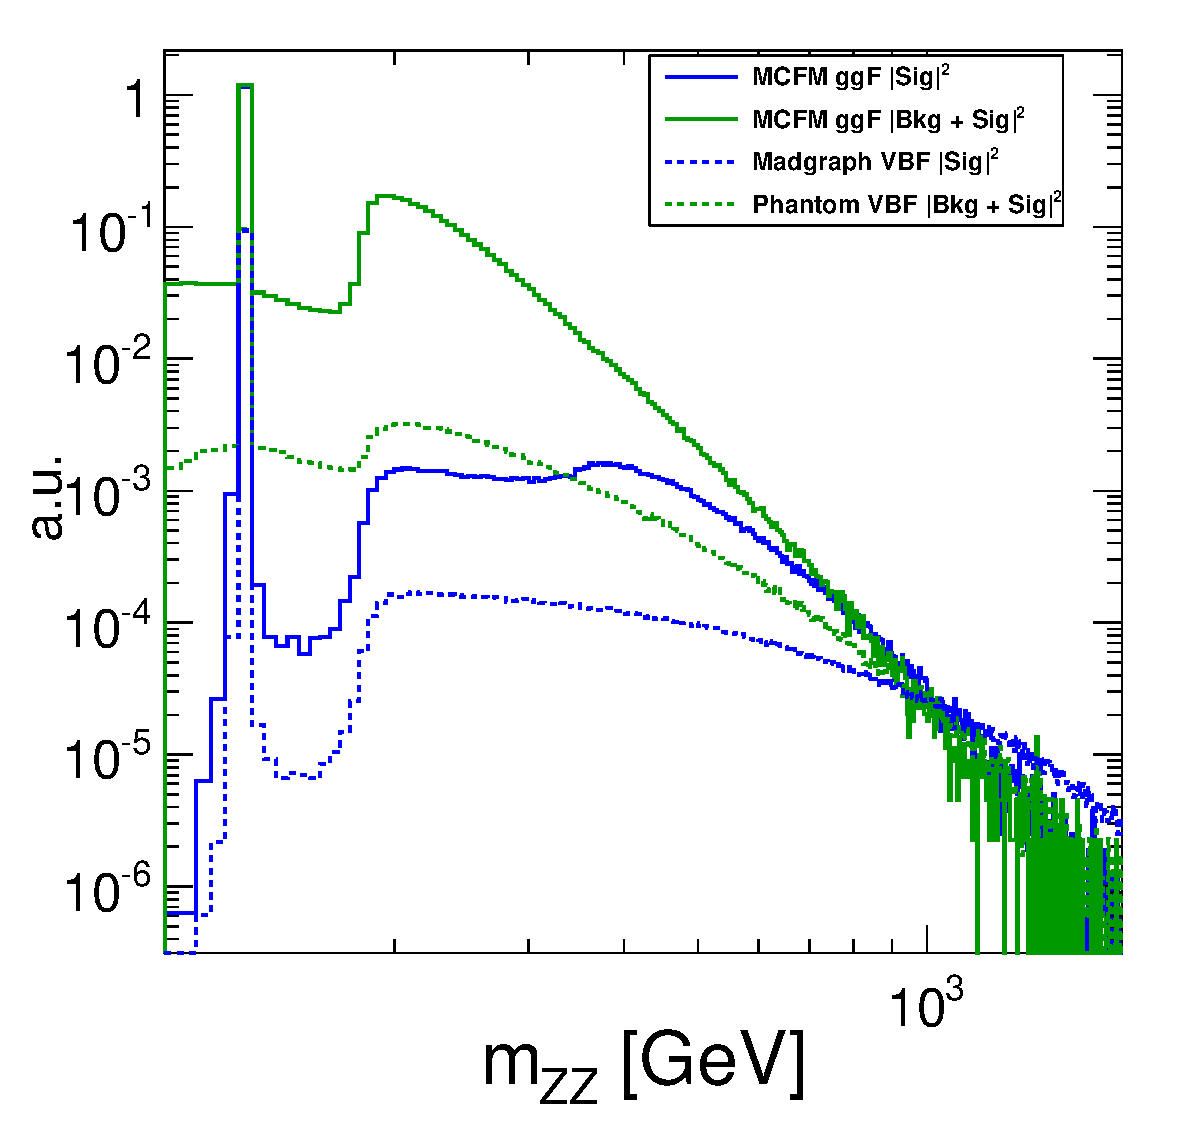
\includegraphics[width=.45\linewidth]{HiggsProperties/figures/ggFvVBF_log_fix.eps}
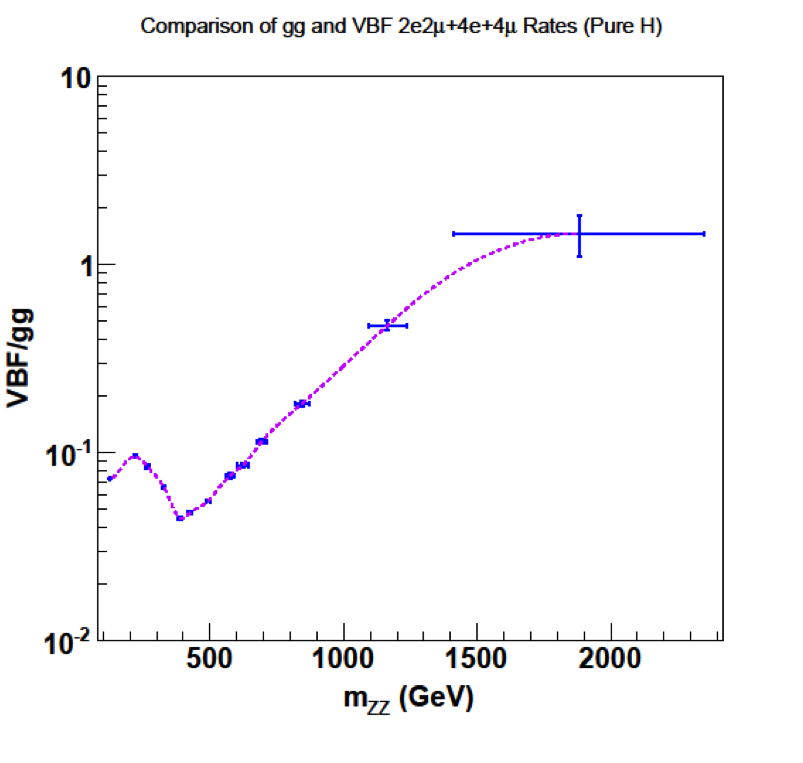
\includegraphics[width=.45\linewidth]{HiggsProperties/figures/vbf2.png}
\caption[Comparisons Between VBF and ggF Productions for Off-Shell Region]{On left, differential cross sections for ggF (signal-only [solid blue] and signal plus background with interference [solid green] both from {\tt MCFM}) and VBF (signal-only shape [dashed blue] from {\tt MadGraph}, signal plus background with interference [dashed green] from {\tt Phantom}). As $m_{4\ell}$ increases, the VBF contributions become more dominant, seen in the ratio between VBF and gluon-gluon fusion in the right plot.}
\label{fig:VBFvggF_OffShell}
\end{center}
\end{figure}

Since these background samples are produced at leading order, we need to apply a scale factor to bring the effective cross section to NNLO. As discussed in Sec.~\ref{sec:HighMass}, the scale factor for the Higgs boson signal sample is known to NNLO-NNLL, but no such scale has been calculated for the background or the interference. However, contrary to the High Mass search, the interference is not rolled directly into the signal mass shape and the scale factor could be independent. Fortunately, a study \cite{Bonvini:1304.3053} found that the same soft-colinear approximation\footnote{Moving to a higher order requires accounting for both additional loops and radiated particles. It has been shown \cite{Kramer:1998} that for gluon fusion, the radiative corrections alone are a good approximation to move to a higher order.} that largely explains the corrections for the signal is also a good description for NNLO effects on the background. By this logic, we can apply the same scale factor uniformly to background, signal, and interference mass distributions. The scale factor applied, as a function of $m_{4\ell}$, is seen in Fig.~\ref{fig:KFactorggF}. Because of the limited theoretical knowledge, a systematic uncertainty of 10\% is applied to this scale factor fro the background. In the on-shell analysis needed for the width measurement, this scale factor has a small impact on the $gg\rightarrow ZZ$ background, but it is applied for consistency. For VBF, an $m_{4\ell}$ independent scale factor is applied to add NNLO QCD corrections of 6\%.

\begin{figure}[htbp]
\begin{center}
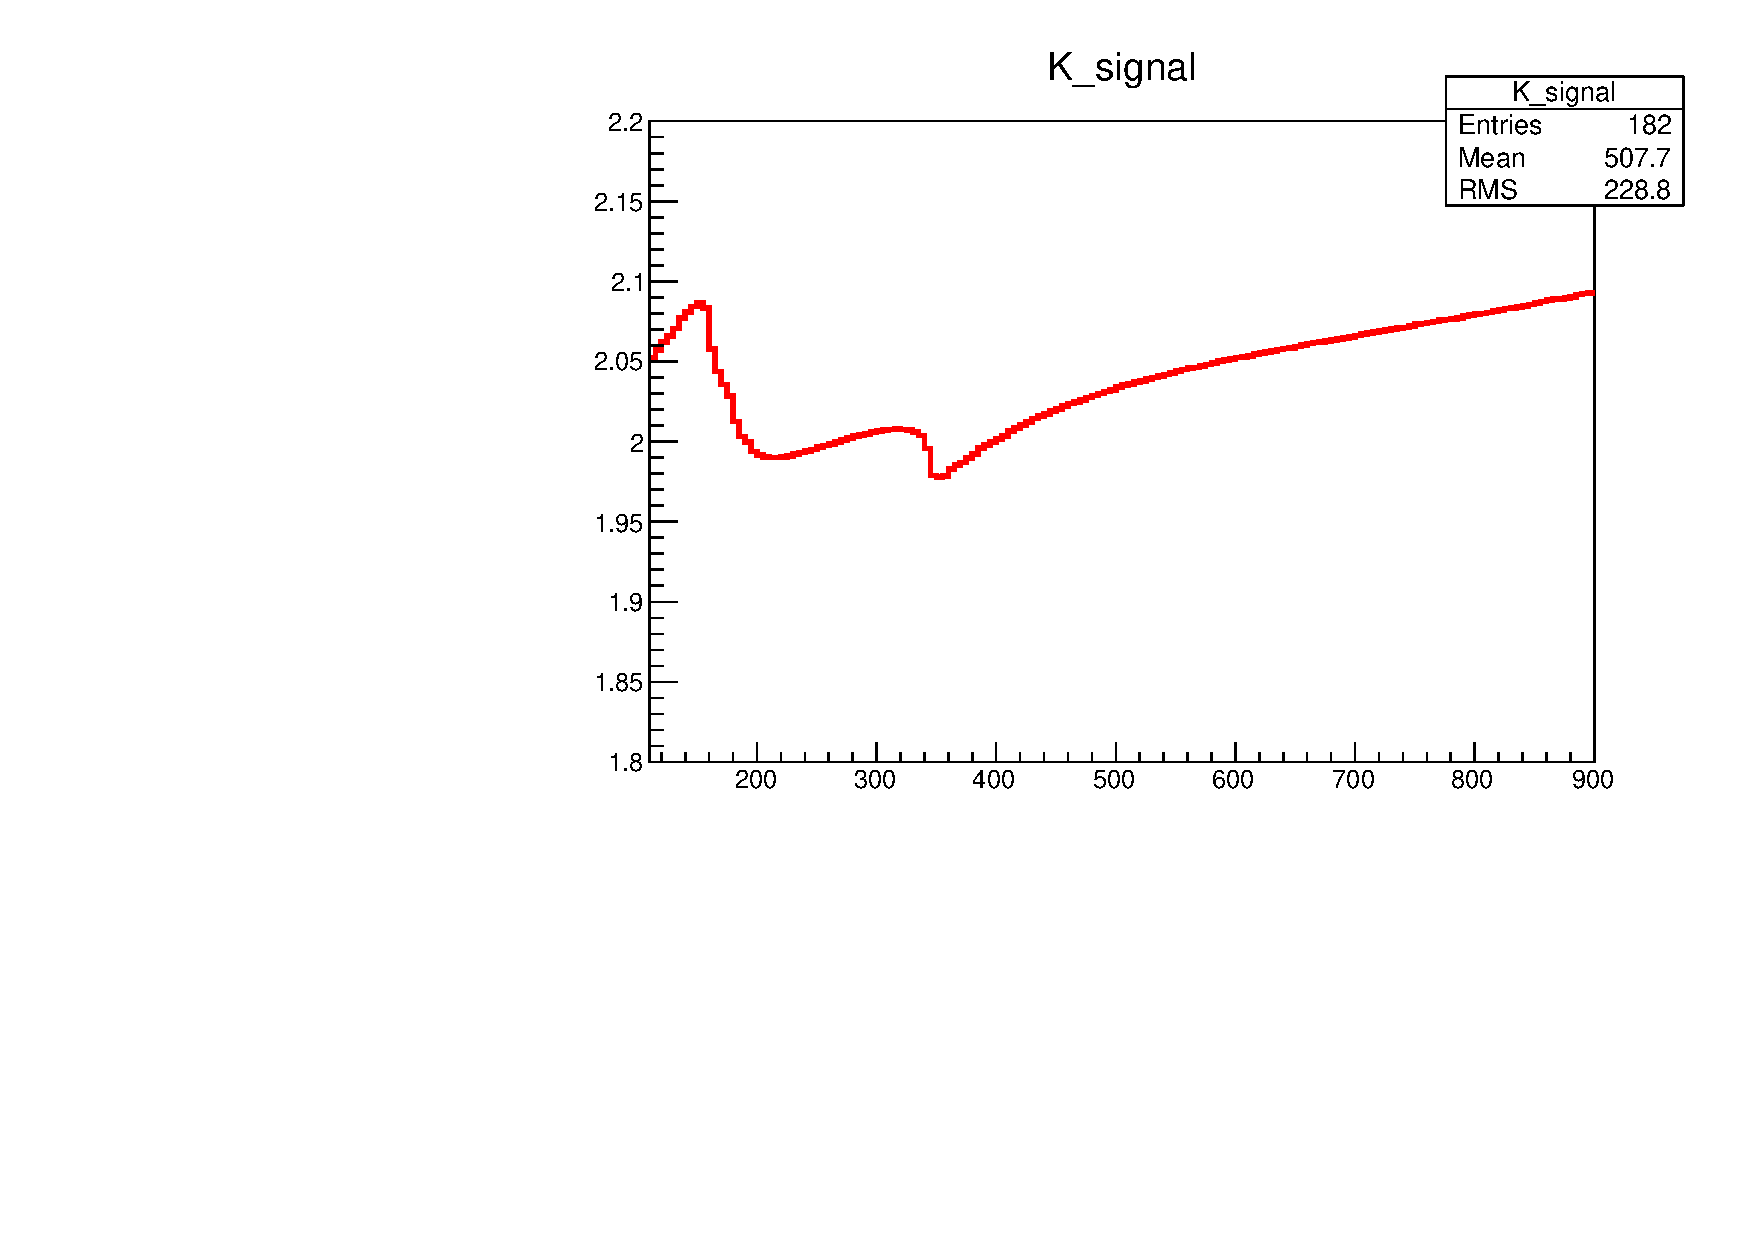
\includegraphics[width=.5\linewidth]{HiggsProperties/figures/kfactorpassa.pdf}
\caption[NNLO/LO Scale Factor at 8 $\rm{TeV}$ for ggF Signal]{Scale factor used to move from LO to NNLO for ggF 8 $\rm{TeV}$ signal. This factor is applied identically for signal, background, and interference. The scale factor was also calculated for 7 $\rm{TeV}$, where the shape is the same but with a magnitude of about 1.6.}
\label{fig:KFactorggF}
\end{center}
\end{figure}

To conduct the off-shell analysis, the statistical analysis also needs to be modified from Sec.~\ref{sec:ZZ4lAnalysis} or Sec.~\ref{sec:HighMass} as we are no longer looking for localized resonances but broad excesses over the high mass region. Each high mass event ($m_{4\ell}\geq220$ $\rm{GeV}$) is assigned a likelihood for the probability that it belongs to a particular signal (ggF or VBF), background, or interference:
\begin{equation}
\mathcal{L}_{\rm off-shell} = N_{ggZZ}\mathcal{P}_{\rm sig+bkg+int}^{ggZZ} + N_{VBF}\mathcal{P}_{\rm sig+bkg+int}^{VBF} + N_{q\bar{q}ZZ}P_{bkg}^{q\bar{q}} + N_{ZX}\mathcal{P}_{bkg}^{ZX}
\label{eqn:GenOffShellLikelihood}
\end{equation}
where $N_{x}$ refers to the number of expected events\footnote{For $gg\rightarrow4l$ and VBF, the numbers of events depend on the signal strength and thus are fitted values.} and $\mathcal{P}^{x}$ is the associated normalized probability distribution function for each process. For $N_{x}$, it is computationally expensive to generate MC samples for every value of $r$. Instead, we use the relation of Eqn.~\ref{eqn:OffShellDiff_ZZ} for the number of total $gg/VV \rightarrow 4\ell$ events in terms of the SM signal, background, and interference contributions,
\begin{equation}
N_{\rm tot} = r \times N_{\rm sig} + \sqrt{r}\times N_{\rm int} + N_{\rm bkg}. 
\label{eqn:NOffShell}
\end{equation}
The left plot of Fig.~\ref{fig:NOffShell} shows that the analytic model is in very good agreement with the sample points generated for different values of $r$. This allows $N_{\rm tot}$, and therefore the likelihood, to be determined for an arbitrary value of $r$. An additional closure test using Eqn.~\ref{eqn:OffShellDiff_ZZ} on the differential cross sections from generated MC samples is shown in the right plot of Fig.~\ref{fig:NOffShell}.

\begin{figure}[htbp]
\begin{center}
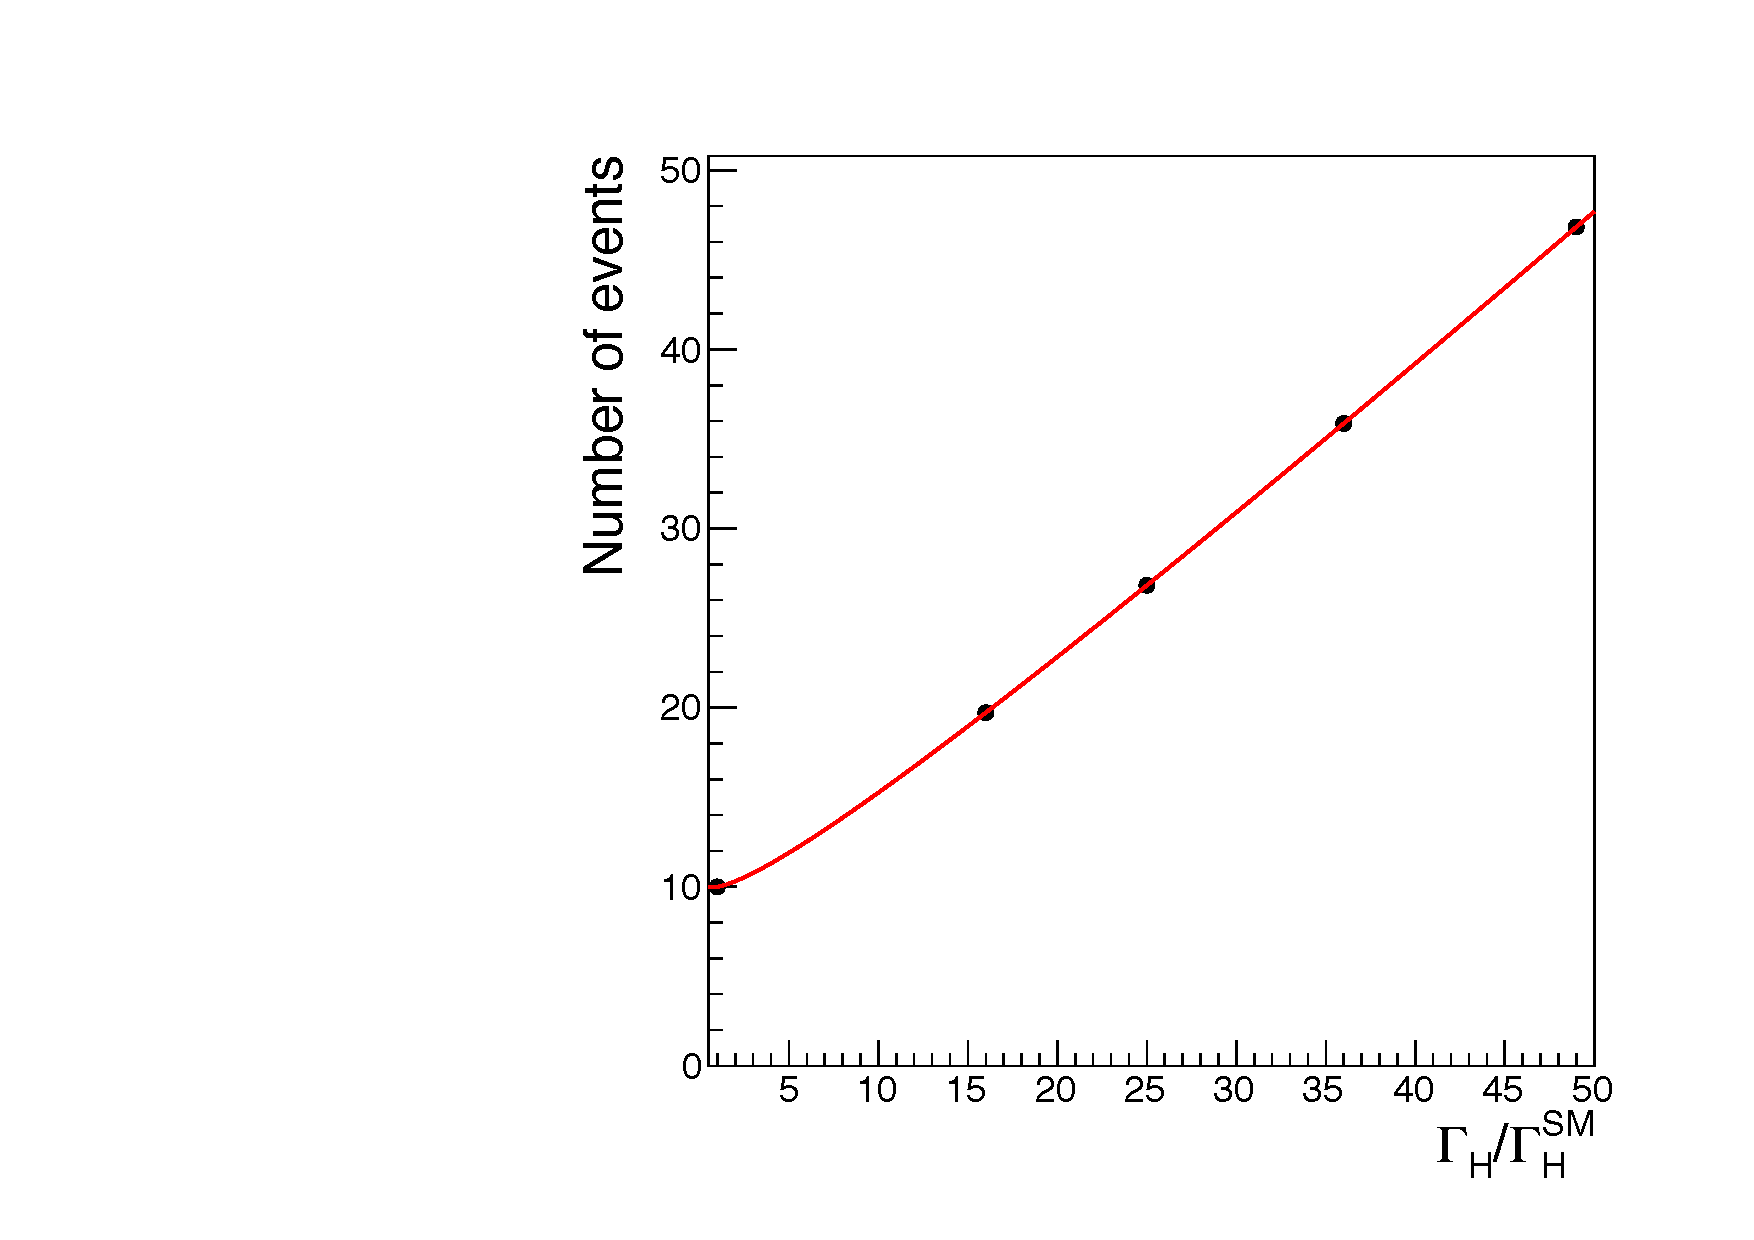
\includegraphics[width=.45\linewidth]{HiggsProperties/figures/yield.pdf}
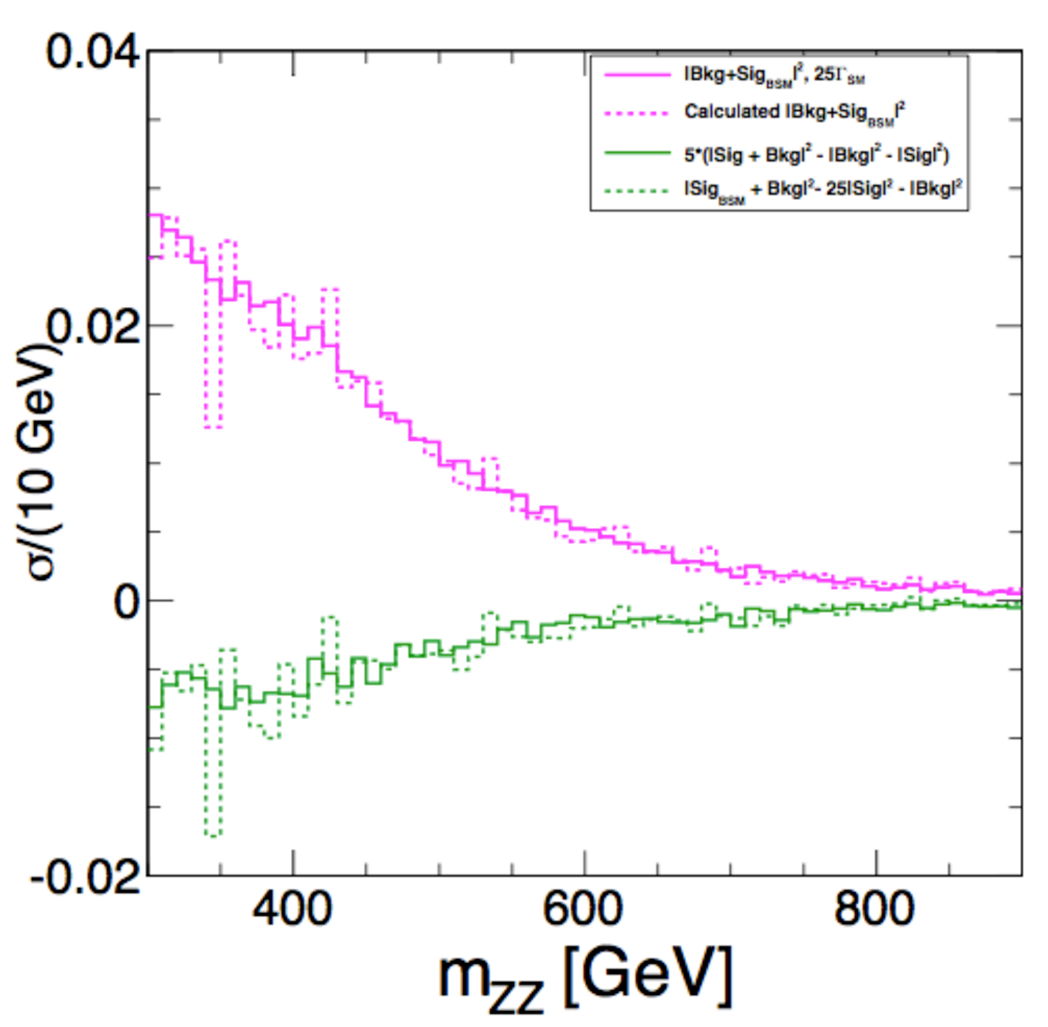
\includegraphics[width=.45\linewidth]{HiggsProperties/figures/closuretestNHetNI.pdf}
\caption[Modeling of Off-Shell Normalizations in $4\ell$]{On left, an analytic model, Eqn.~\ref{eqn:NOffShell} (red), for the total number of signal + background + interference events for $gg$ or $VV\rightarrow 4\ell$ as a function of the width compares very well to five points generated via MC. On right, a closure test where the differential cross sections from MC (solid) is compared against calculated shapes from other samples (dashed). Good agreement is seen both in the shape for the signal + background with interference (magenta) and isolated interference (green) for $r=25$.}
\label{fig:NOffShell}
\end{center}
\end{figure}

In the on-shell analysis, we used three dimensions $(m_{4\ell},\mathcal{D}_{\rm{bkg}}^{\rm{kin}},p_T \mathrm{~or~} \mathcal{D}_{\rm jet})$ via an analytic $m_{4\ell}$ shape and two 2D templates to build these probability distributions. In principle, the same observables could be used here. However, as we are trying to isolate any $gg\rightarrow 4\ell$ process\footnote{Recall that for the decay kinematics, there should be nearly no difference between VBF and ggF.} from the $q\bar{q}\rightarrow 4\ell$ background, we should build a different discriminant to separate these two distributions.  

Using the MELA approach outlined in Sec.~\ref{sec:HVVDecay}, we build two probabilities for our discriminant:
\begin{align}
\mathcal{P}_{gg,a}(\vec{\Omega},m_1,m_2|m_{4\ell},m_{H}) &= a\times\mathcal{P}_{sig}^{gg} + \sqrt{a}\times\mathcal{P}_{\rm int}^{gg} + \mathcal{P}_{\rm bkg}^{gg} \\
\mathcal{P}_{q\bar{q}}(\vec{\Omega},m_1,m_2|m_{4\ell},m_{H}) &= \mathcal{P}_{\rm bkg}^{q\bar{q}}
\end{align}
where each probability $\mathcal{P}$ depends on the standard set of decay kinematics and masses $(\vec{\Omega},m_{4\ell},m_H)$ used in Sec.~\ref{sec:ZZ4lKD} with $m_H=125.6$ $\rm{GeV}$. The parameter $a$ corresponds to the effective signal strength where the Standard Model expectations give $a=1$. These probabilities are calculated using the MELA package, based on JHUGen and MCFM matrix elements. Then, the new discriminant for the off-shell analysis is:
\begin{equation}
\mathcal{D}_{gg,a} \equiv \frac{\mathcal{P}_{gg,a}}{\mathcal{P}_{gg,a}+\mathcal{P}_{q\bar{q}}} = \left[1 + \frac{\mathcal{P}_{\rm bkg}^{q\bar{q}}}{a\times\mathcal{P}_{\rm sig}^{gg} + \sqrt{a}\times\mathcal{P}_{\rm int}^{gg} + \mathcal{P}_{\rm bkg}^{gg}}\right]^{-1}
\end{equation}
where, following the usual procedure, a correction factor $c(m_{4\ell})$ is included in $\mathcal{P}_{\rm bkg}^{q\bar{q}}$ such that the sum of the probabilities above and below $\mathcal{D}_{gg,a}=0.5$ are equal. For this discriminant, the value of $a$ must be optimized and should be near the target exclusion of $r$. Initial studies indicated that $r=10$ sensitivity is possible and that the results do not change substantially when $a$ is varied up or down by a factor of 2, so we set $a=10$ and adopt the shorthand $\mathcal{D}_{gg} \equiv \mathcal{D}_{gg,10}$.

For the probabilities in Eqn.~\ref{eqn:GenOffShellLikelihood}, we use this discriminant in 2D templates of $(m_{4\ell},\mathcal{D}_{gg})$ in the off-shell analysis, found via MC\footnote{The {\tt Phantom} samples were not fully simulated by the time of this analysis, so two methods were used to build the VBF templates: reweighting the {\tt MCFM} samples using the right plot of Fig.~\ref{fig:VBFvggF_OffShell} and momentum smearing of the {\tt Phantom} samples to mimic detector effects. The variation between these two methods become the dominant shape systematic in the VBF templates.} (or control region for $Z+X$). The on-shell analysis maintains the same 3D distributions as before. We could use $\mathcal{D}_{\rm jet}$ as well for the off-shell analysis to separate the production mechanisms of any observed off-shell signal events. As the first measurement of width using the off-shell region, we are primarily looking for an excess of Higgs boson-like events which have similar decay kinematics, so to simplify computation we do not use $\mathcal{D}_{\rm jet}$ in this study, but we will revisit the production mechanism in Sec.~\ref{sec:OffShellAnom}. Sample templates of $(m_{4\ell},\mathcal{D}_{gg})$ are seen in Fig.~\ref{fig:2DWidthTemplates}.

\begin{figure}[htbp]
\begin{center}
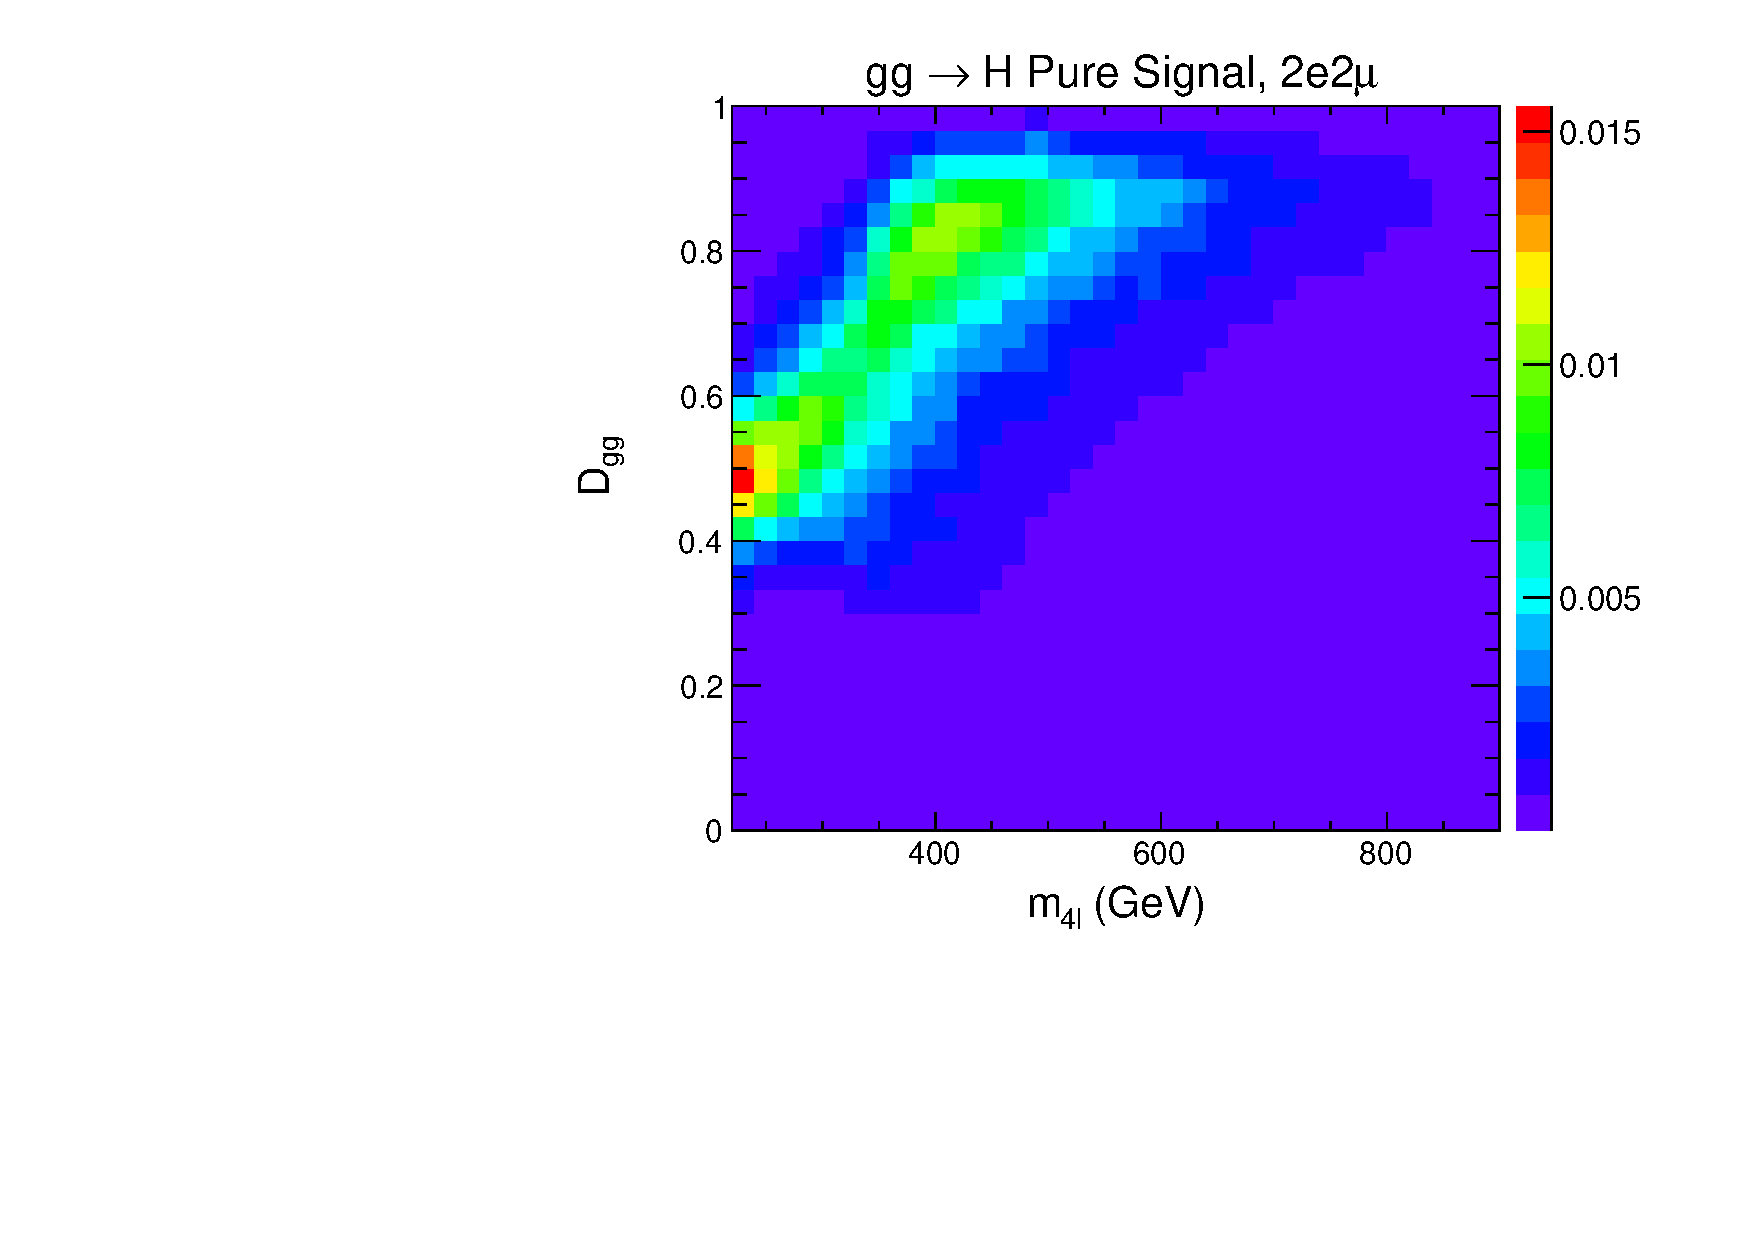
\includegraphics[width=.3\linewidth]{HiggsProperties/figures/2DtemplateggH.pdf}
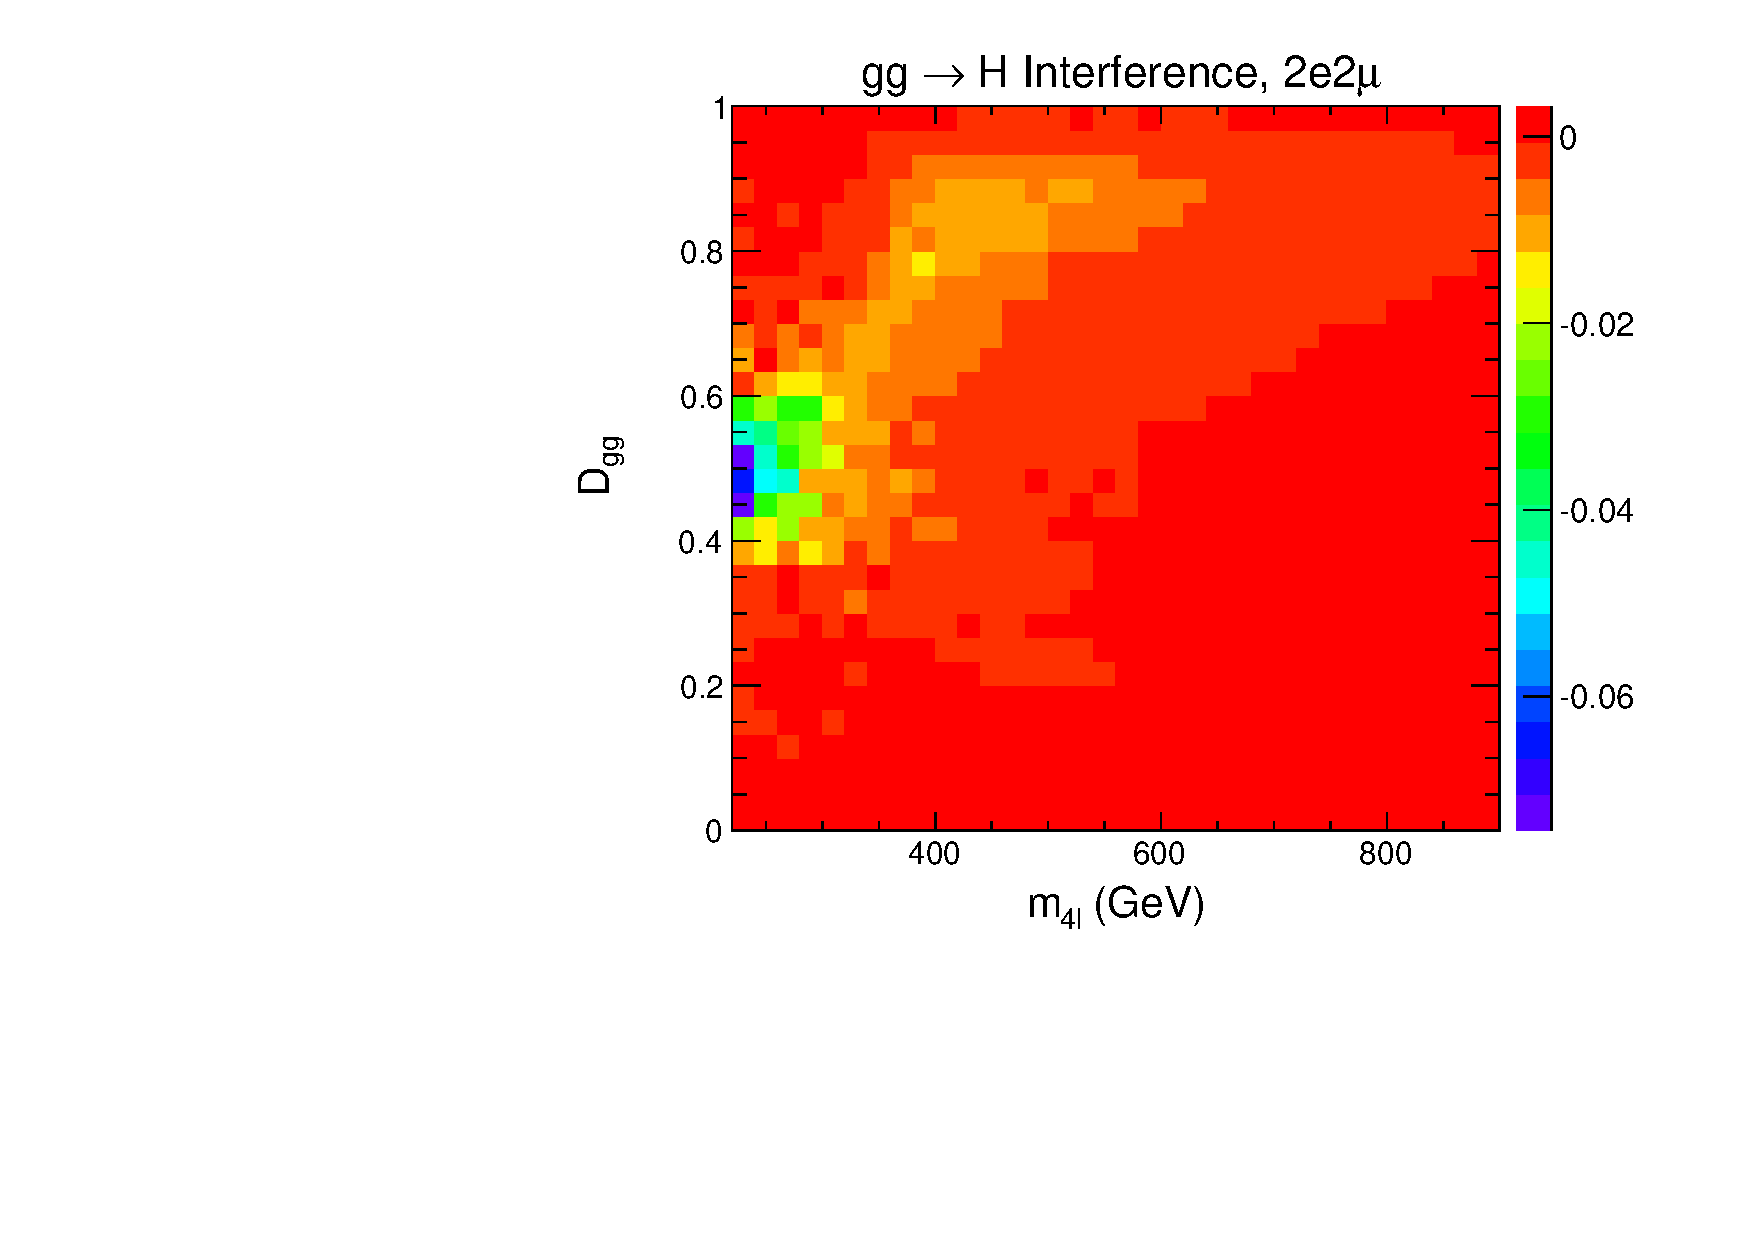
\includegraphics[width=.3\linewidth]{HiggsProperties/figures/2Dtemplateinterf.pdf}
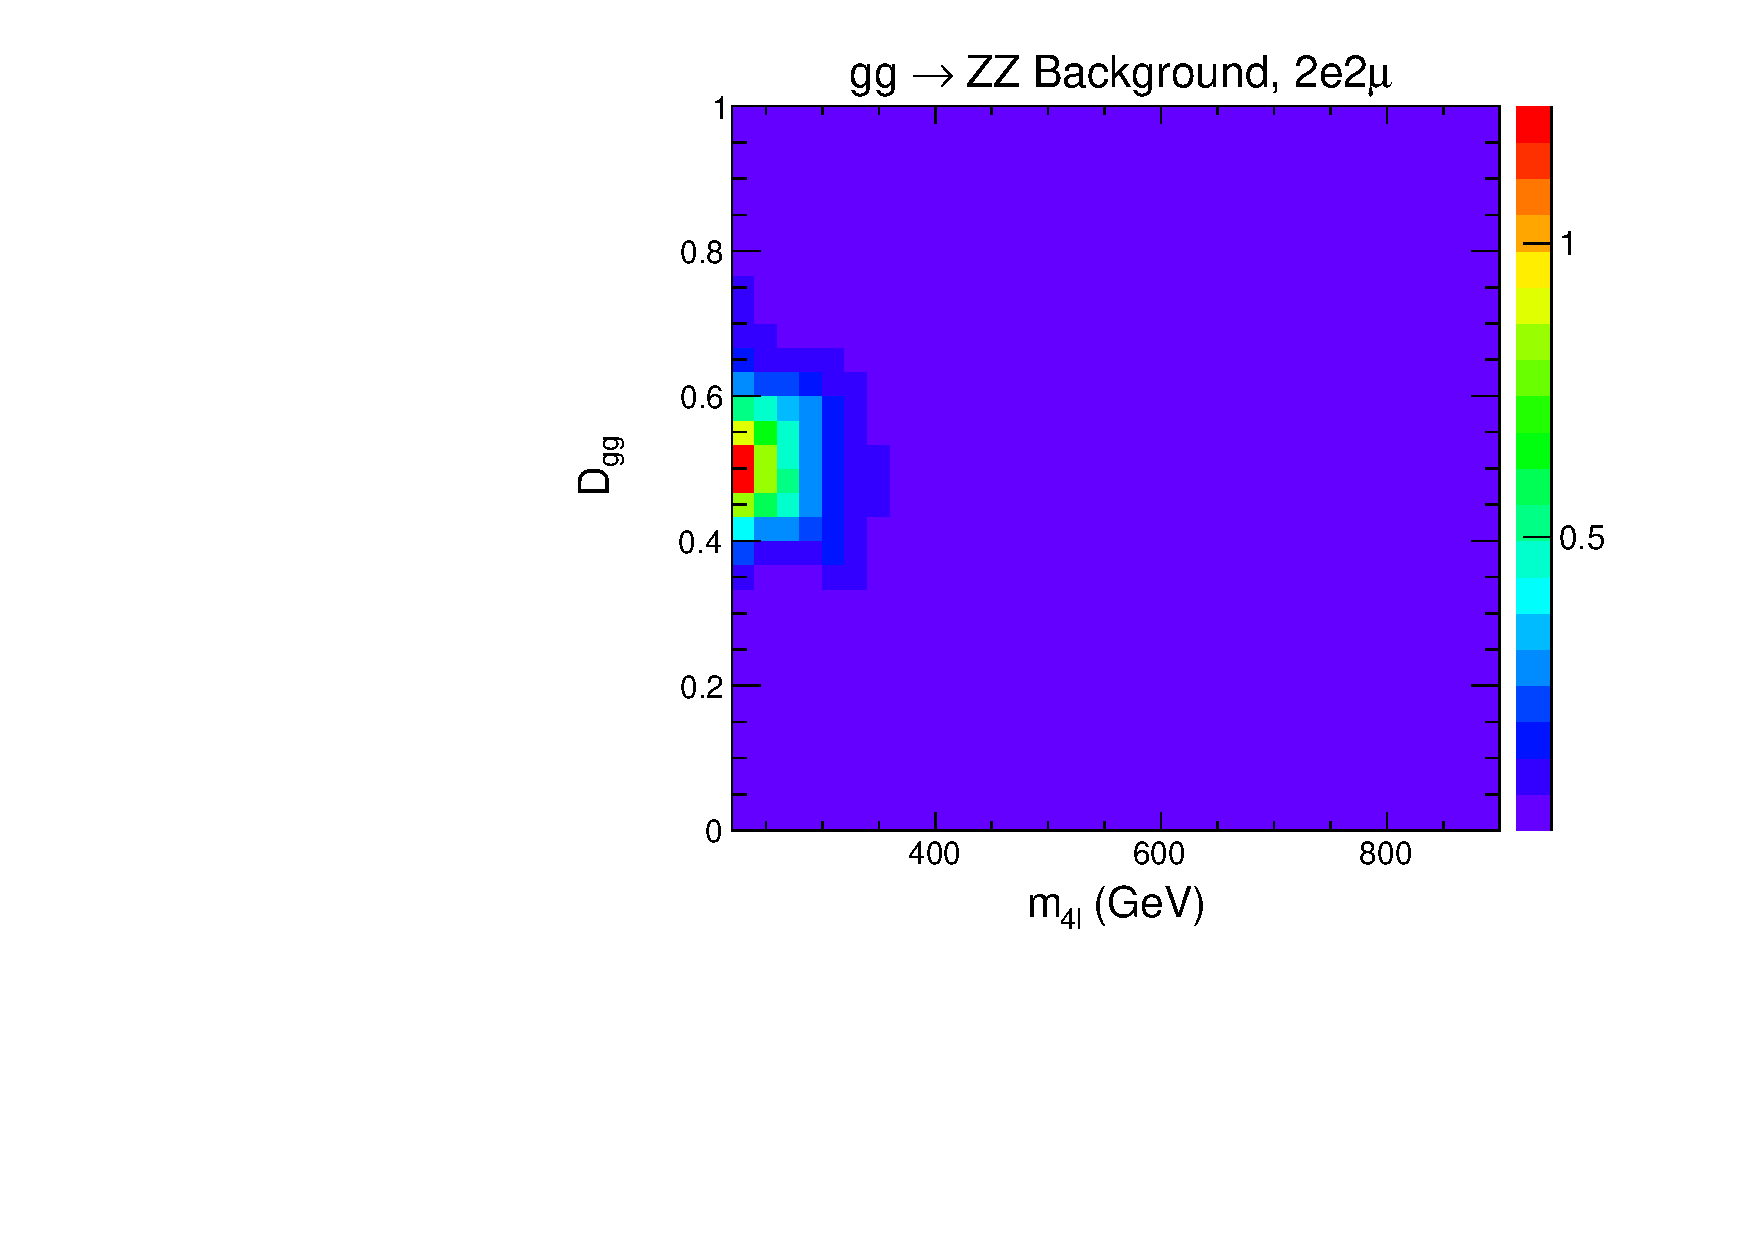
\includegraphics[width=.3\linewidth]{HiggsProperties/figures/2DtemplateggZZ.pdf} \\
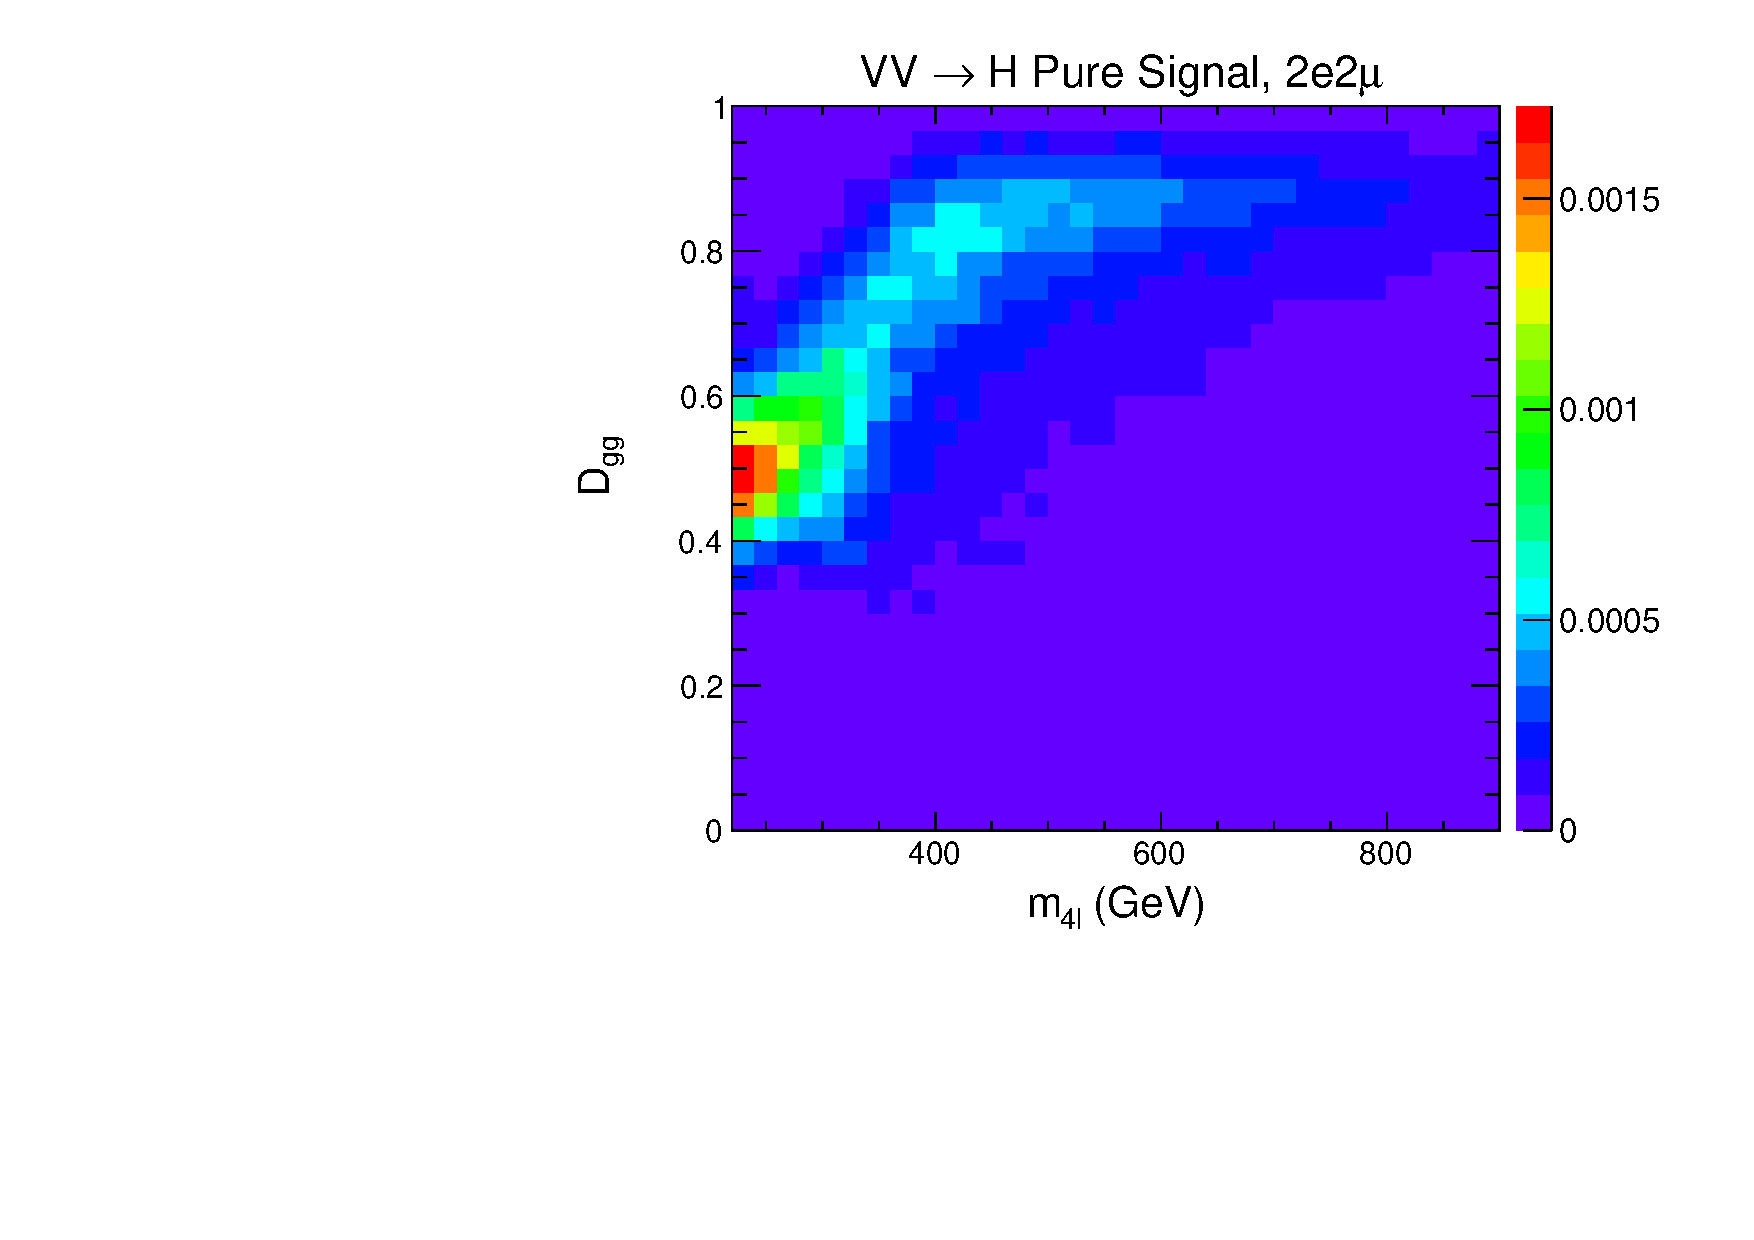
\includegraphics[width=.3\linewidth]{HiggsProperties/figures/2DtemplatevbfH.pdf}
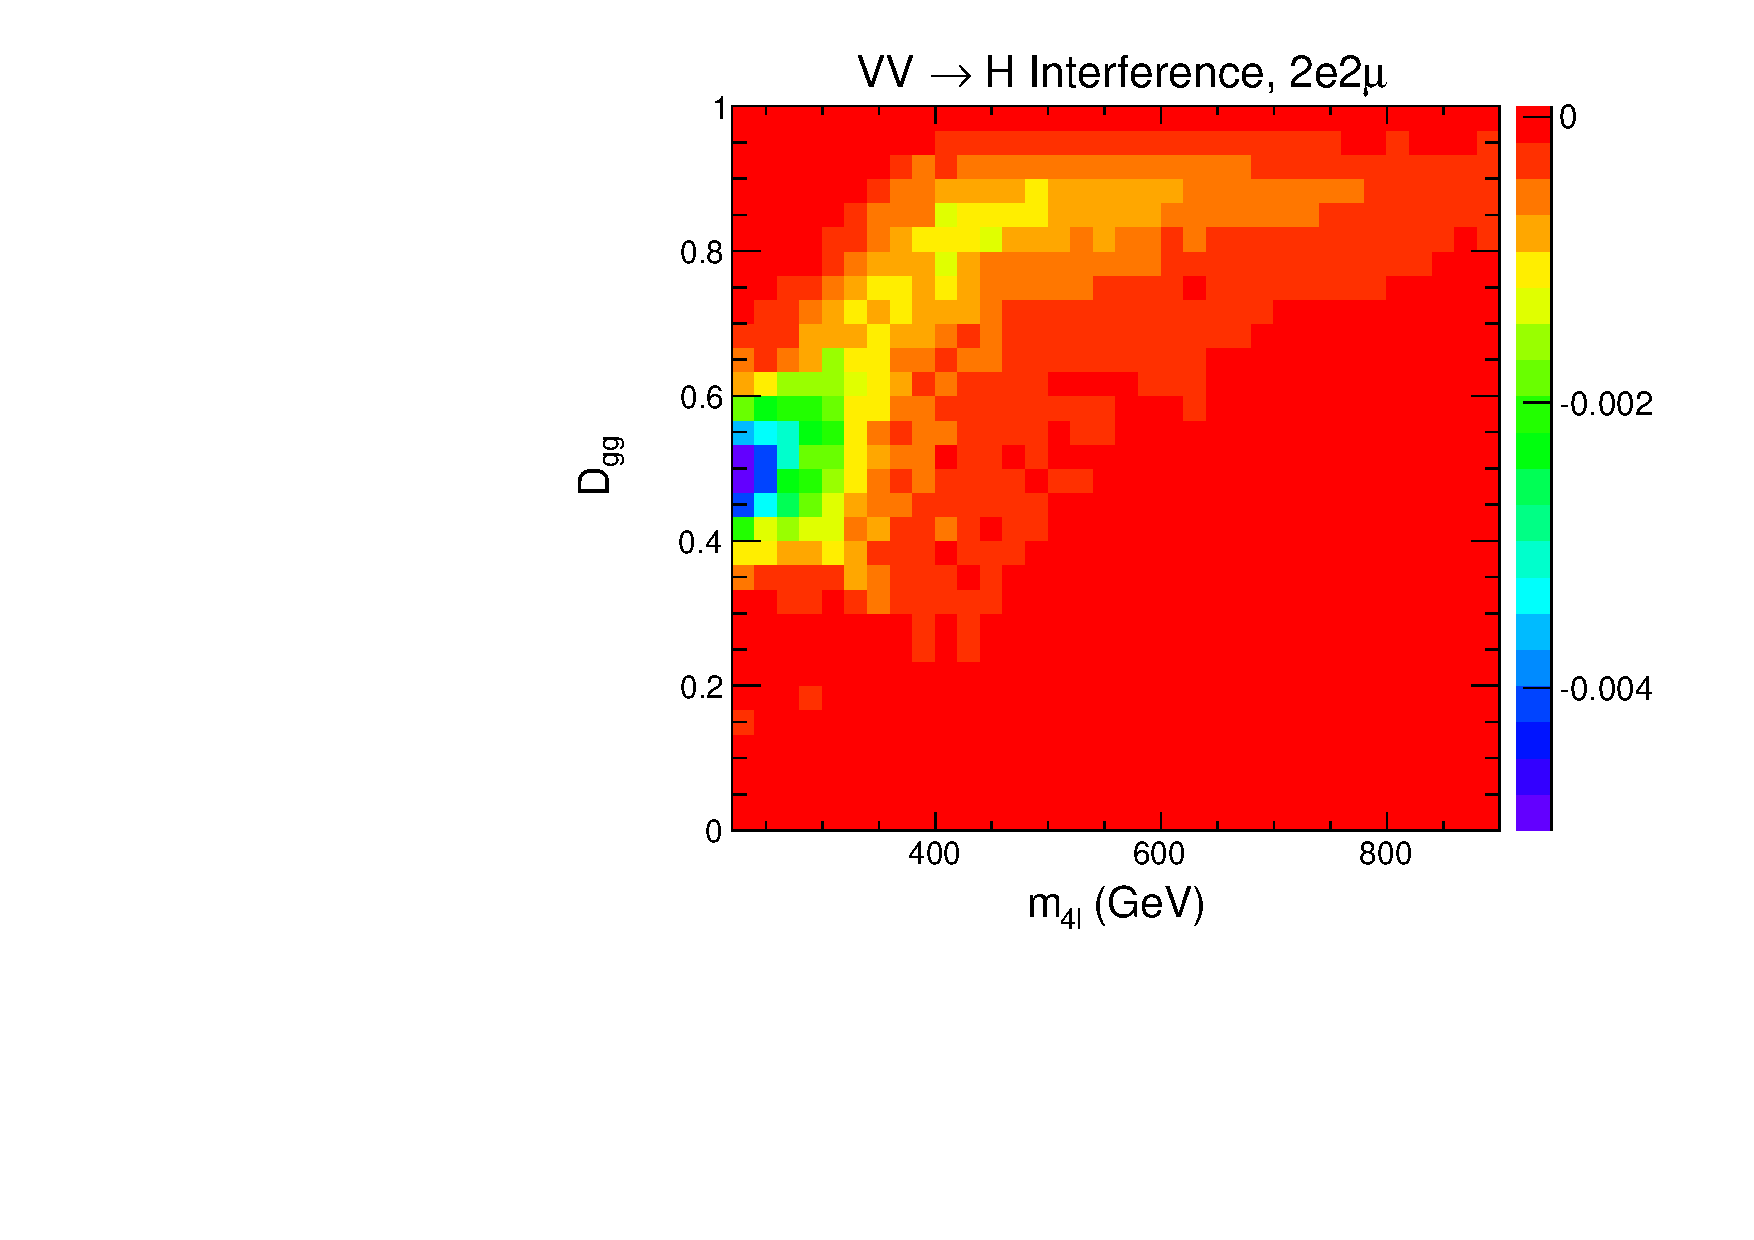
\includegraphics[width=.3\linewidth]{HiggsProperties/figures/2Dtemplateinterfvbf.pdf}
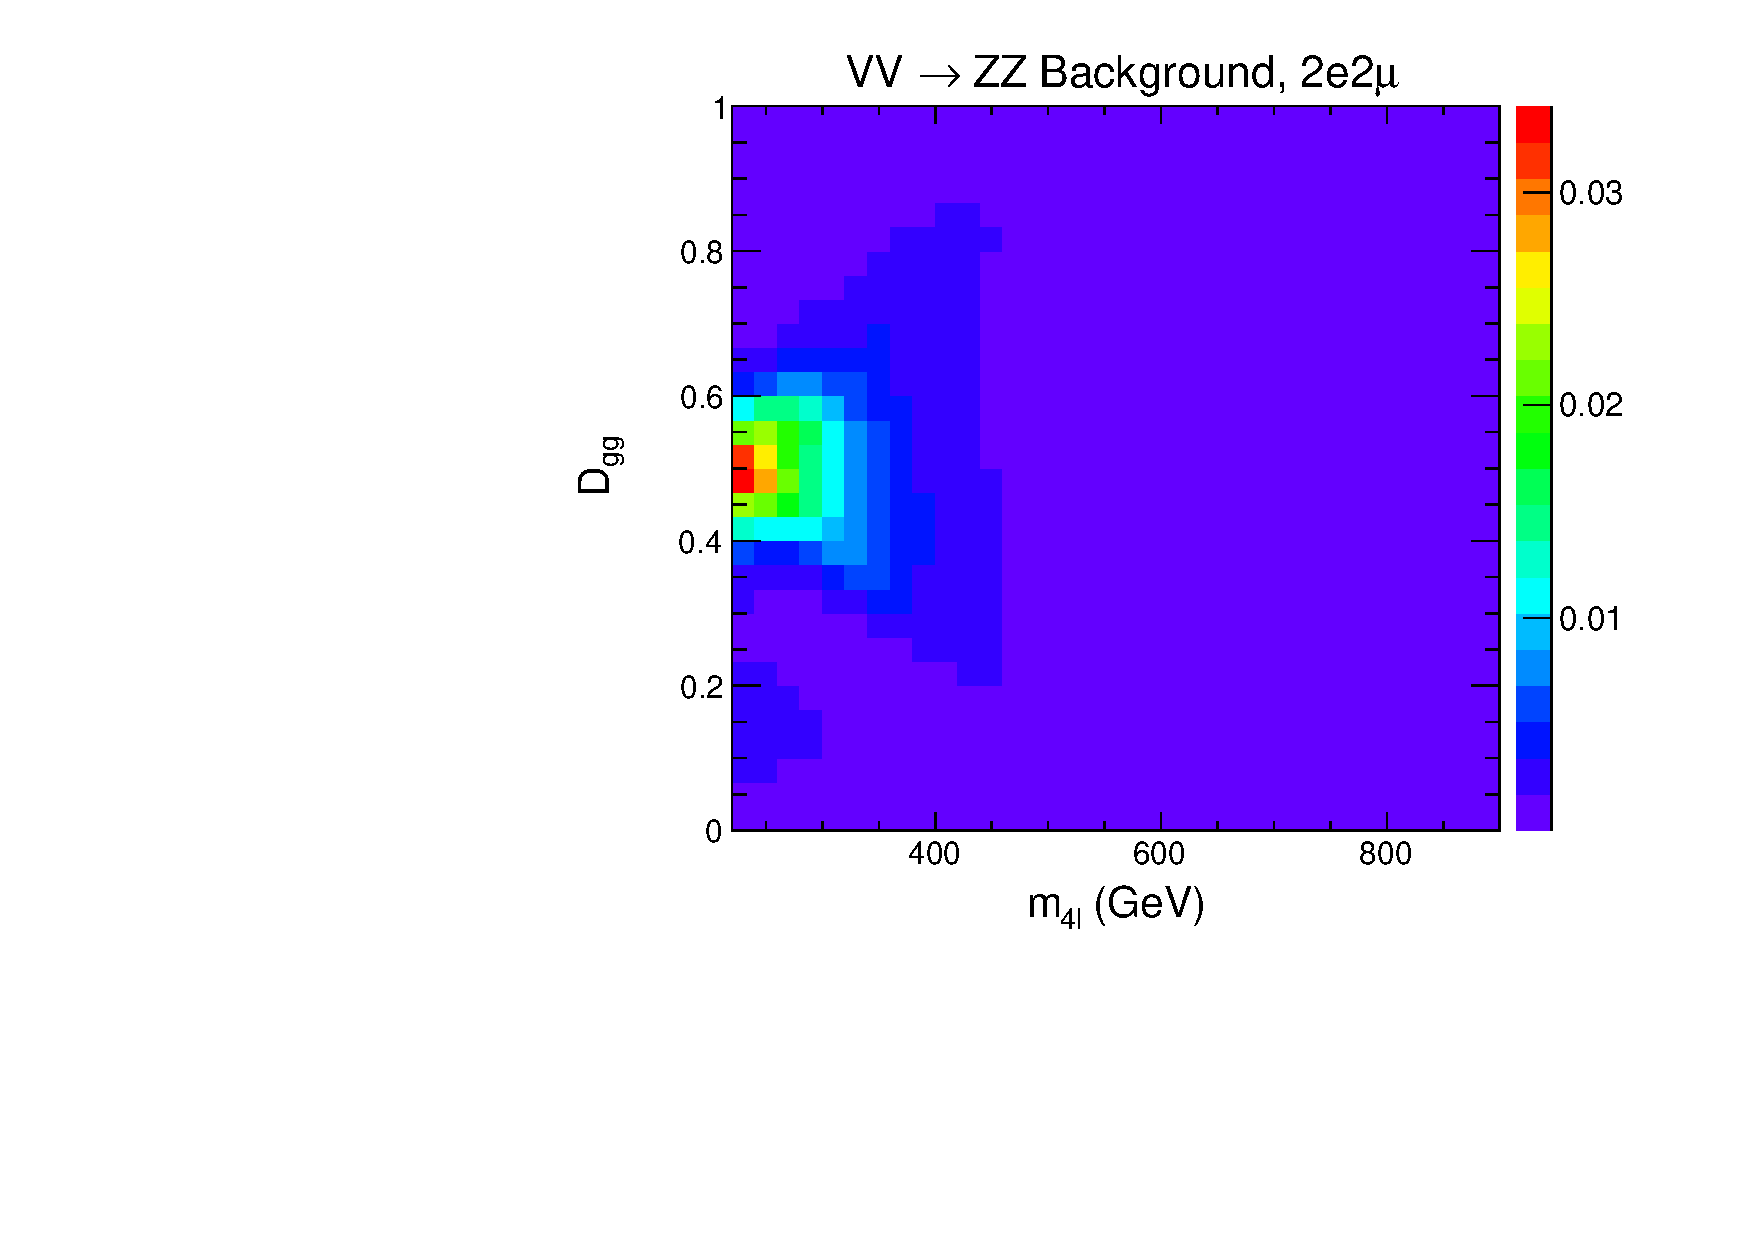
\includegraphics[width=.3\linewidth]{HiggsProperties/figures/2DtemplatevbfZZ.pdf}
\caption[2D $(m_{4\ell},\mathcal{D}_{gg})$ Templates for Off-Shell $4\ell$ Analysis]{$(m_{4\ell},\mathcal{D}_{gg})$ templates for ggF (top row) and VBF (bottom row). Left templates are for signal, middle templates are for interference between signal and background, right templates are for background. The interference is destructive, as indicated by the color negative values in the templates. Additional templates are made for the $q\bar{q}\rightarrow4\ell$ and $Z+X$ backgrounds.}
\label{fig:2DWidthTemplates}
\end{center}
\end{figure}

Thus, the probabilities for VBF and ggF processes in Eqn.~\ref{eqn:GenOffShellLikelihood} take the form:
\begin{equation}
\mathcal{P}_{\rm sig+bkg+int}^{\rm prod} = \left[r\mu\times\mathcal{P}_{\rm sig}^{\rm prod} + \sqrt{r\mu}\times\mathcal{P}_{\rm int}^{\rm prod} + \mathcal{P}_{\rm bkg}^{\rm prod} \right]
\end{equation}
where the probability distributions are the constructed $(m_{4\ell},\mathcal{D}_{gg})$ templates. Crucially, the interference template will be negative to account for destructive interference. However, negative probabilities are non-physical, so the full probability $\mathcal{P}_{\rm sig+bkg+int}^{\rm prod}$ is normalized to be 1 for $r\mu=1$ so it is positive-definite. Given these details, the likelihood of Eqn.~\ref{eqn:GenOffShellLikelihood} can be rewritten as
\begin{equation}
\begin{split}
\mathcal{L}_{\rm off-shell} &= N_{ggZZ}\left[r\mu_{F}\times\mathcal{P}_{\rm sig}^{gg} + \sqrt{r\mu_{F}}\times\mathcal{P}_{\rm int}^{gg} + \mathcal{P}_{\rm bkg}^{gg}\right] \\
&+ N_{VBF}\left[r\mu_{V}\times\mathcal{P}_{\rm sig}^{VBF} + \sqrt{r\mu_{V}}\times\mathcal{P}_{\rm int}^{VBF} + \mathcal{P}_{\rm bkg}^{VBF}\right] \\
&+ N_{q\bar{q}ZZ}P_{bkg}^{q\bar{q}} + N_{ZX}\mathcal{P}_{bkg}^{ZX}
\end{split}
\end{equation}
where $\mu_V$ and $\mu_F$ are the bosonic and fermionic signal strengths, respectively.

Aside from the aforementioned changes, there are a few minor modifications to the systematics listed in Sec.~\ref{sec:ZZ4lSystematics}. For the $q\bar{q}\rightarrow ZZ$ background, NLO electroweak corrections \cite{Baglio:1307.4331,Bierweiler:1312,Gieseke:2014gka} not available in the earlier analysis of Sec.~\ref{sec:ZZ4lMCandData} are applied in the nominal $q\bar{q}\rightarrow ZZ$ mass distribution, seen in Fig.~\ref{fig:qqZZEWKCorrections}. The interplay between the electroweak corrections and QCD corrections is not known theoretically, so following \cite{kasprzikpriv}, we implement an uncertainty equal to the product of the two corrections. The factorization, normalization, and signal scale factors were allowed to vary up and down by a factor of 2, where the scale factor uncertainty comes from \cite{Passarino:2013bha} and the other variations come from the {\tt MCFM} and {\tt GG2VV} generators. For the 2D templates, alternative shapes were built using different PDF sets and the NLO QCD scale variations. Lastly, any systematics that should affect both on-shell and off-shell regions (e.g. normalization) are set to be 100\% correlated.

\begin{figure}[htbp]
\begin{center}
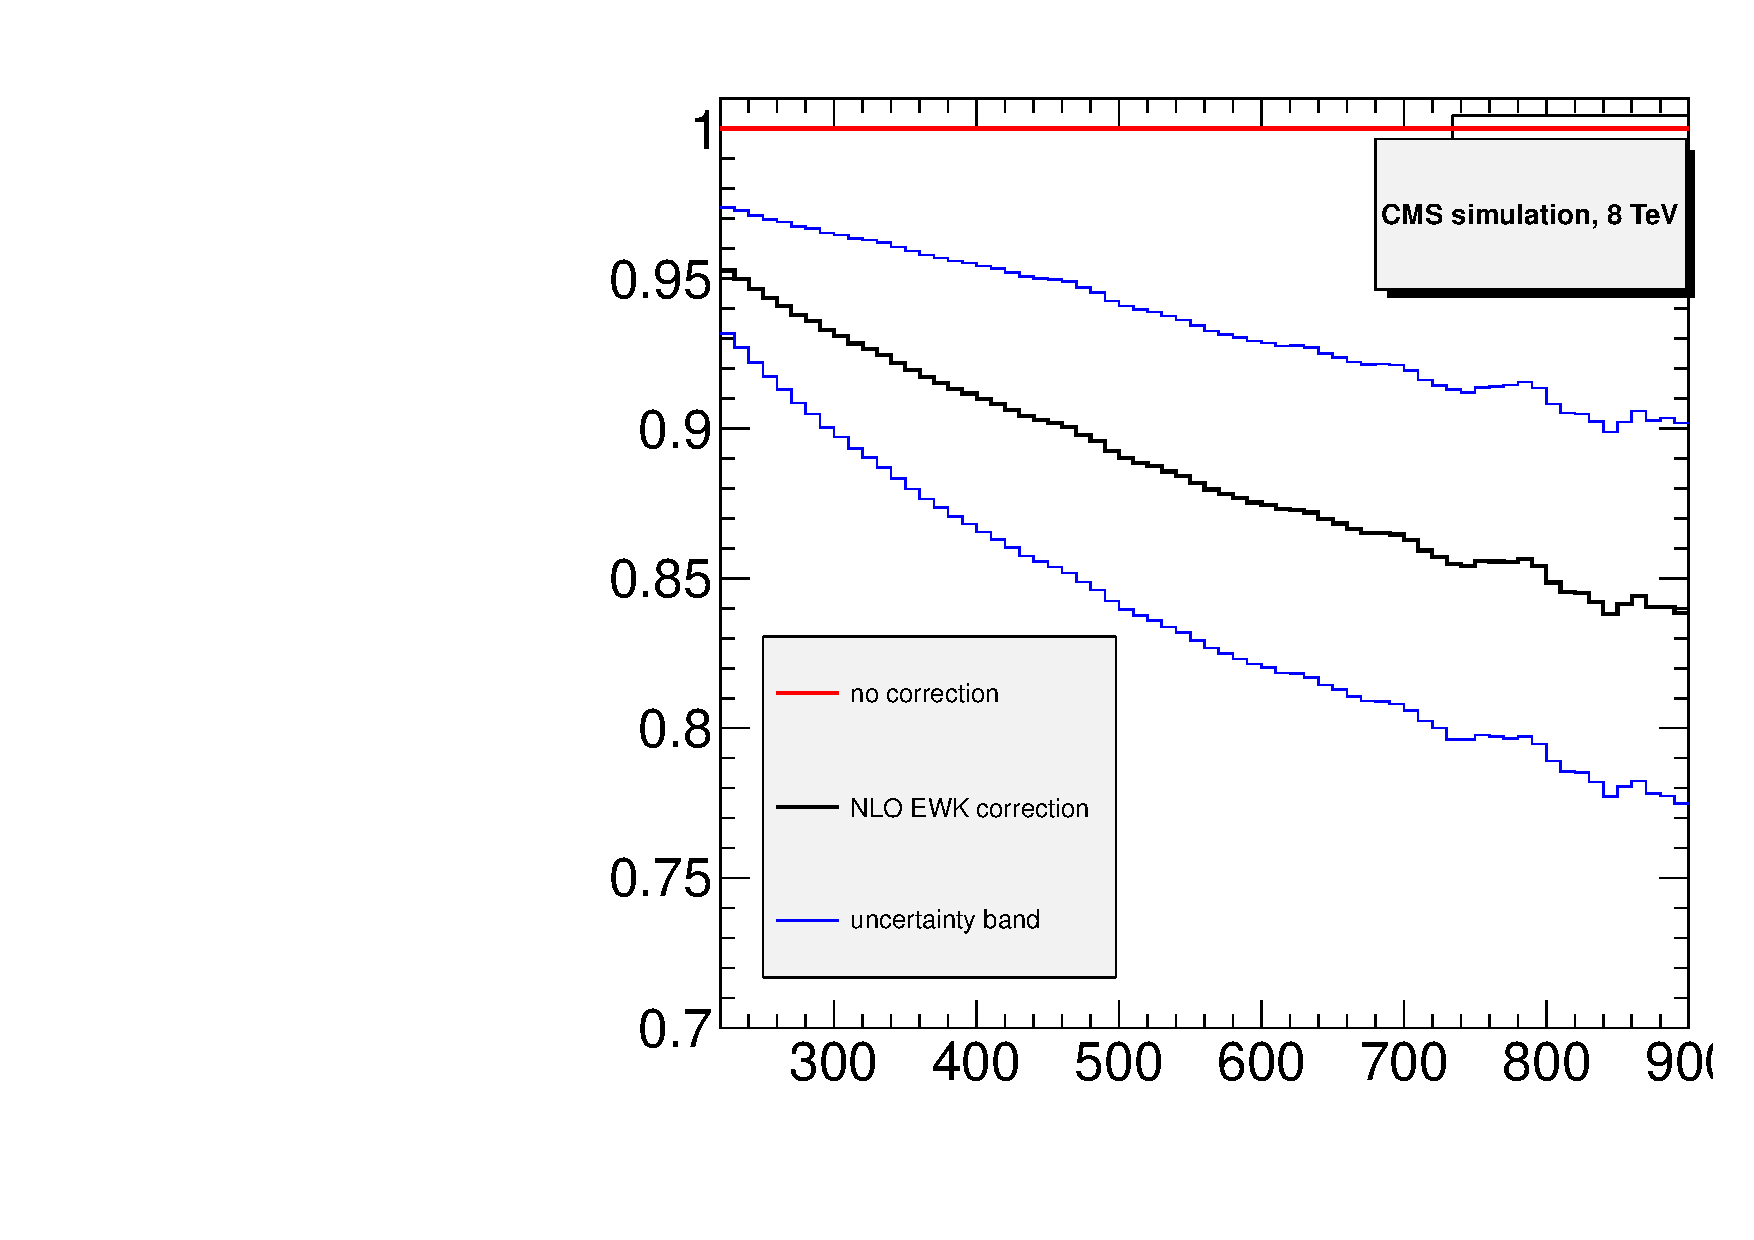
\includegraphics[width=.5\linewidth]{HiggsProperties/figures/EWKcorr_ratio.pdf}
\caption[NLO Electroweak Corrections for $q\bar{q}\rightarrow ZZ$ Background]{NLO electroweak corrections for the $q\bar{q}\rightarrow ZZ$ background as a ratio of the uncorrected background in terms of $m_{4\ell}$. The shape used in on-shell analysis (Sec.~\ref{sec:ZZ4lMassShape}) was not corrected (red) as it was published before these corrections were available. A new nominal $q\bar{q}\rightarrow ZZ$ shape was built using the ratio these corrections to the uncorrected shape (black) and $\pm1\sigma$ uncertainty bands (blue), coming from correlations between QCD and electroweak corrections.}
\label{fig:qqZZEWKCorrections}
\end{center}
\end{figure}

With this analysis in place, we first will look for any large excess of Higgs boson-like events in the off-shell region that would indicate an anomalously large width. Then, using those results, we can simultaneously maximize the likelihoods of the on-shell and off-shell regions to measure the width in the case of an excess or set an upper limit if no excess is observed.

\subsection{Width Measurement Using Off-shell Analysis}
\label{sec:WidthResults}

Utilizing the analysis defined in Sec.~\ref{sec:OffShellAnalysis}, the distribution of $7$ and $8$ $\rm{TeV}$ events over the full $m_{4\ell}$ range is shown in Fig.~\ref{fig:Width4l_Full} with a table of the expected and observed numbers of events are in Table~\ref{tbl:OffShell4lYields}. There appears to be a slight excess of events near the $2\times m_{Z}$ peak, but there are no broad excesses that would indicate an anomalously large width. Given that the off-shell Higgs mass shape plateaus for $m_{4\ell} > 2\times m_{Z}$ and that these signal events would have larger values of $\mathcal{D}_{gg}$, we plot the distributions for $m_{4\ell}>330$ $\rm{GeV}$ and $\mathcal{D}_{gg}>0.65$ in Fig.~\ref{fig:Width4l_SignalEnriched}, where the yields in this signal-enriched region are in the rightmost column of Table~\ref{tbl:OffShell4lYields}.

\begin{figure}[htbp]
\begin{center}
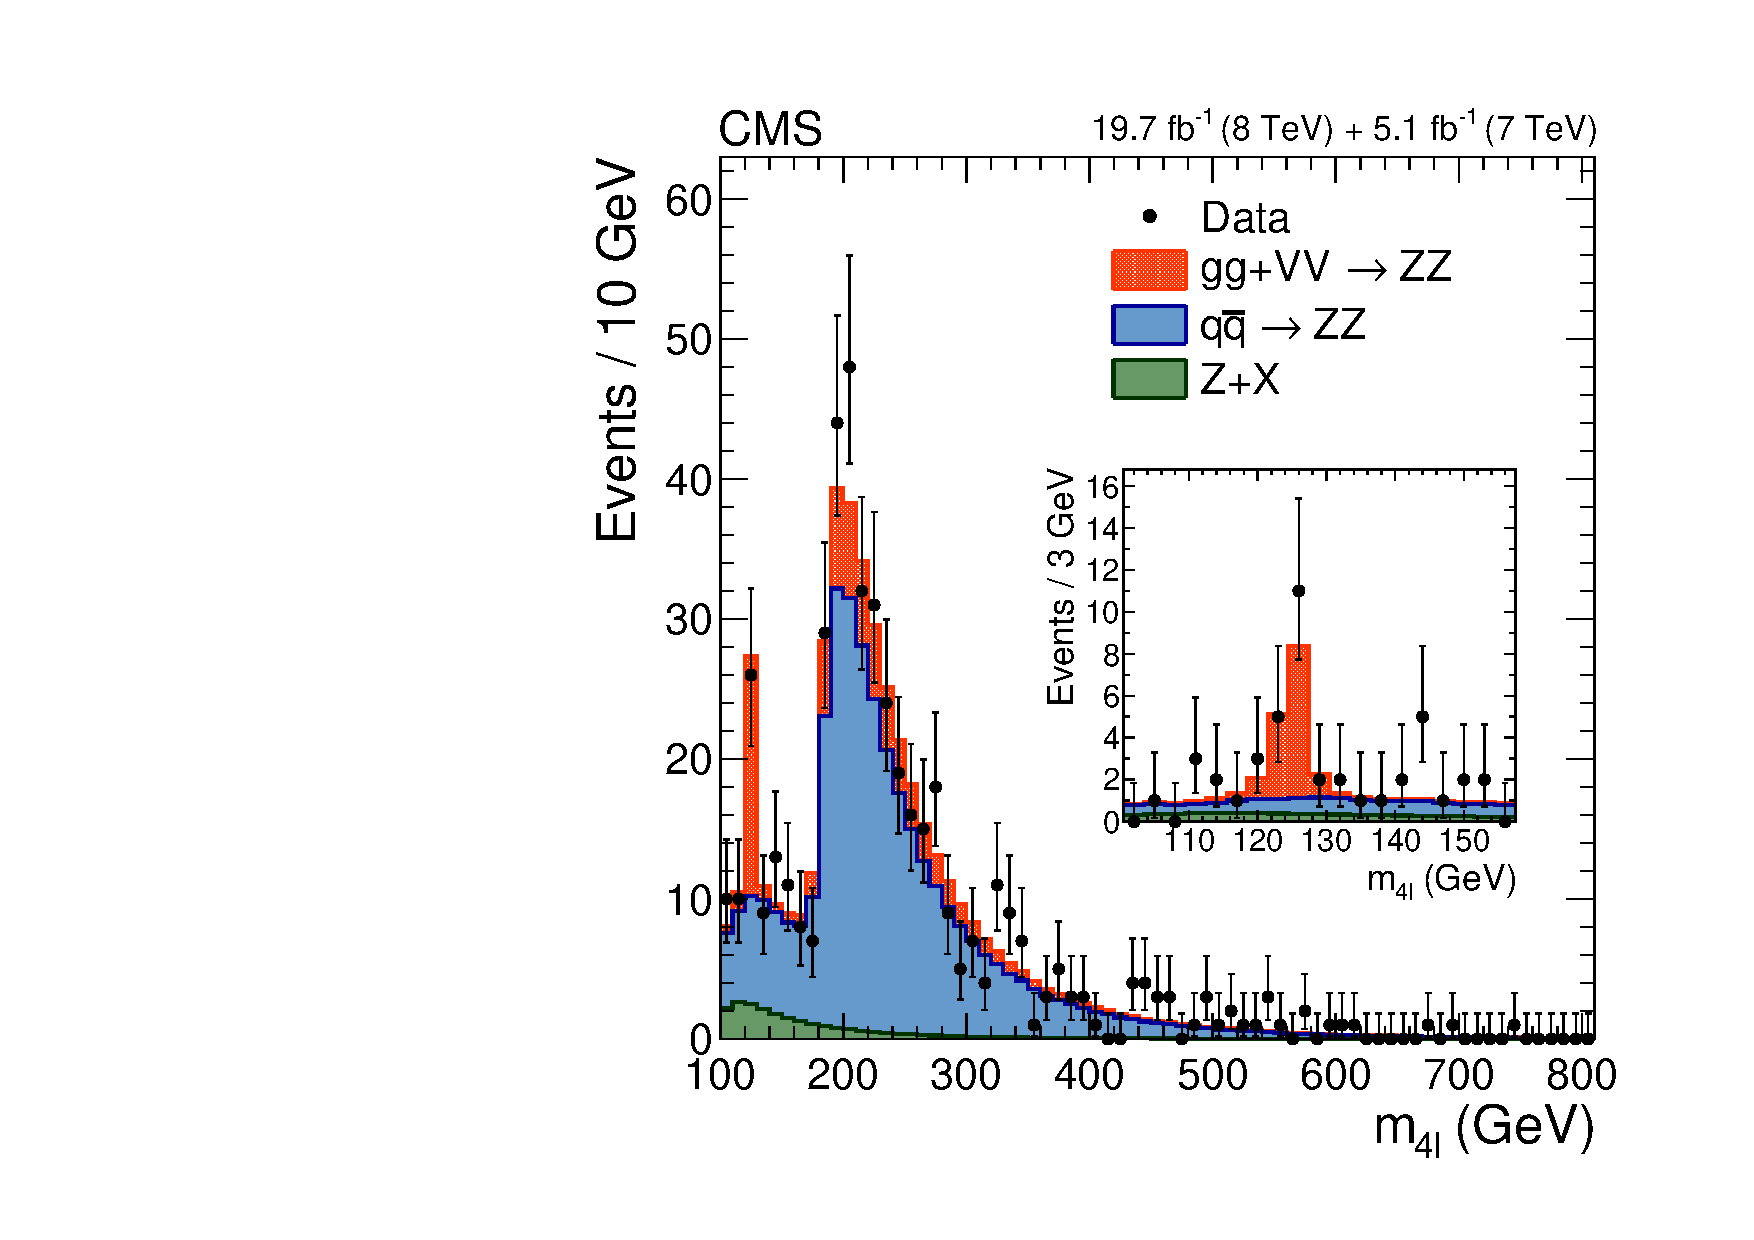
\includegraphics[width=.8\linewidth]{HiggsProperties/figures/fig2_new.pdf}
\caption[$m_{4\ell}$ Distributions of Expected and Observed $4\ell$ Events in the On-Shell and Off-Shell Regions]{Observed $4\ell$ events (black points) for on-shell and off-shell regions, $100<m_{4\ell}<800$ $\rm{GeV}$, with expected distributions with SM-like Higgs boson. $gg + VV \rightarrow ZZ$ distributions (red) account for signal, background, and interference for ggF and VBF production methods. $q\bar{q}\rightarrow ZZ$ (blue) and $Z+X$ (green) are the dominant and sub-dominant backgrounds for the width measurement. The inlaid plot is a narrow region near the Higgs boson peak, $100<m_{4\ell}<160$ $\rm{GeV}$, where only observed and expected events for $\mathcal{D}_{\rm{bkg}}^{\rm{kin}}>0.5$ are plotted. No broad excesses at high mass indicative of an anomalously large width are observed.}
\label{fig:Width4l_Full}
\end{center}
\end{figure}

\renewcommand{\arraystretch}{0.8}
\begin{table}[htbp]
\begin{center}
\begin{tabular}{l|c|c|c|c|c}
\hline
Final state & 4e  &  2e2$\mu$  & 4$\mu$  & All & Enriched \\
\hline
$gg$ signal (SM) &  $0.50^{+0.07}_{-0.06}$ & $1.19^{+0.13}_{-0.14}$ &  $0.70^{+0.09}_{-0.09}$ &  $2.39^{+0.17}_{-0.19}$ & $1.32^{+0.09}_{-0.10}$ \\
$gg$ background &  $7.5^{+1.4}_{-1.1}$  & $17.9^{+2.8}_{-3.0}$  & $10.8^{+1.6}_{-1.6}$ &  $36.2^{+3.4}_{-3.6}$ & $2.17\pm 0.23$ \\
Total $gg$ (SM) & $7.1^{+1.2}_{-1.2}$ & $17.0^{+2.5}_{-2.6}$ & $9.9^{+1.4}_{-1.6}$ & $34.0^{+3.0}_{-3.1}$ & $1.82^{+0.17}_{-0.18}$ \\
\hline
VBF signal (SM) & $0.048$ & $0.115$ & $0.065$ & $0.228$ & $0.119$ \\                                                                       
VBF background & $0.49$ & $1.17$ & $0.67$ & $2.33$ & $0.34$ \\                                                                             
Total VBF (SM) & $0.43$ & $1.03$ & $0.59$ & $2.05$ & $0.23$ \\
\hline
$q\bar{q}$ & $36.2\pm 4.0$  & $87.9\pm 6.4$  & $53.0\pm 3.6$  & $177.1\pm 8.1$ & $9.5\pm 0.5$  \\
Reducible & $2.2\pm 0.5$ & $1.7\pm 0.4$ & $0.6\pm 0.2$ & $4.5\pm 0.7$ & $0.54\pm 0.09$ \\
\hline
All contributions (SM) & $45.9\pm 4.3$  & $107.6\pm 7.1$ & $64.1^{+3.9}_{-4.0}$  & $217.6\pm 9.5$ & $12.0\pm 0.6$ \\
\hline
Observed  & $41$ & $122$ & $60$ & $223$ & $10$ \\
\hline
\end{tabular}
\caption[Expected and Observed $4\ell$ Yields in Off-Shell Region]{Expected and observed number of events with $m_{4\ell}\geq 220$ $\rm{GeV}$ for each channel and the sum of $4e$, $4\mu$, and $2e2\mu$ channels. Listed expectations are for the Standard Model ($\mu=1$). Total observed events agree with SM expectations within uncertainty. The ``Enriched" column are the number of expected and observed events for the signal-enriched region where $m_{4\ell}\geq 330$ $\rm{GeV}$ and $\mathcal{D}_{gg}>0.65$. No excess is observed for this region.}
\label{tbl:OffShell4lYields}
\end{center}
\end{table}

\begin{figure}[htbp]
\begin{center}
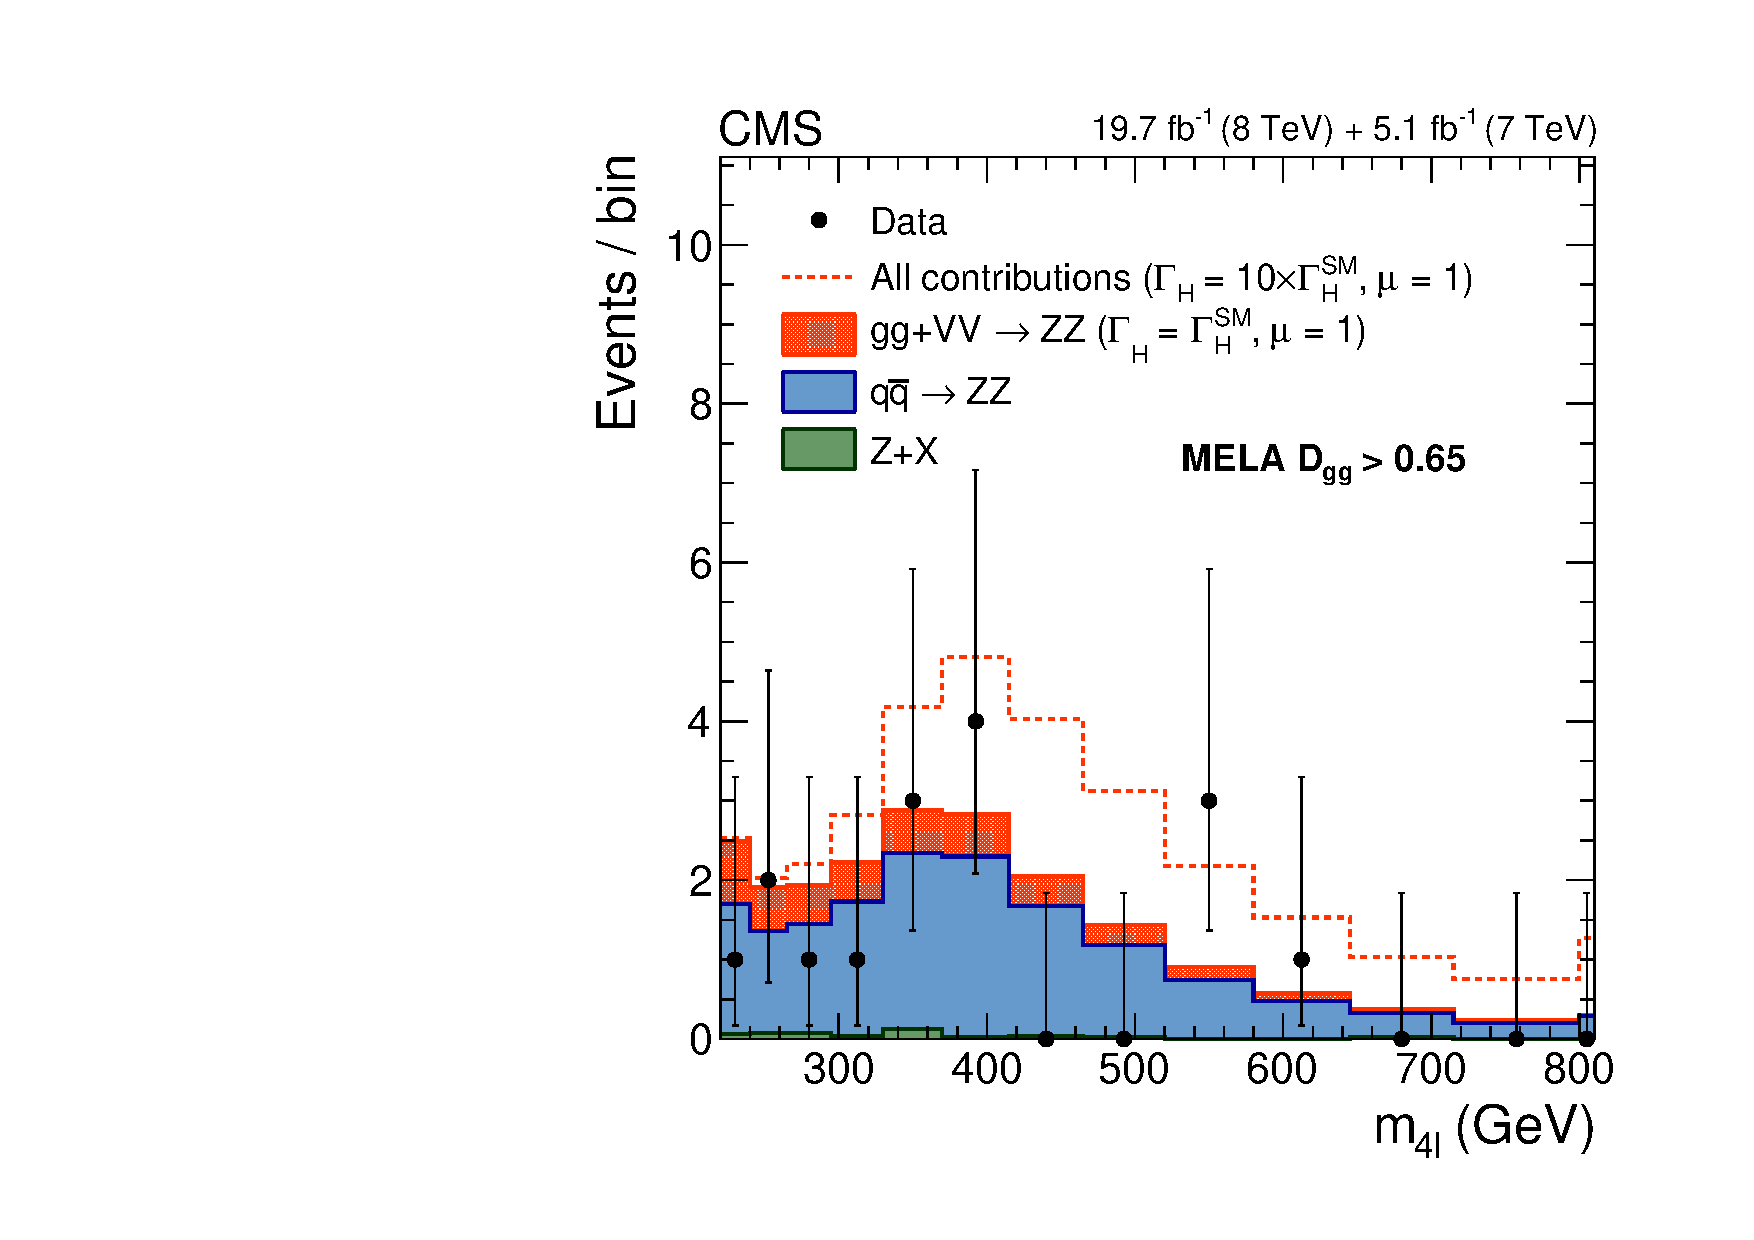
\includegraphics[width=.45\linewidth]{HiggsProperties/figures/fig3a_new.pdf}
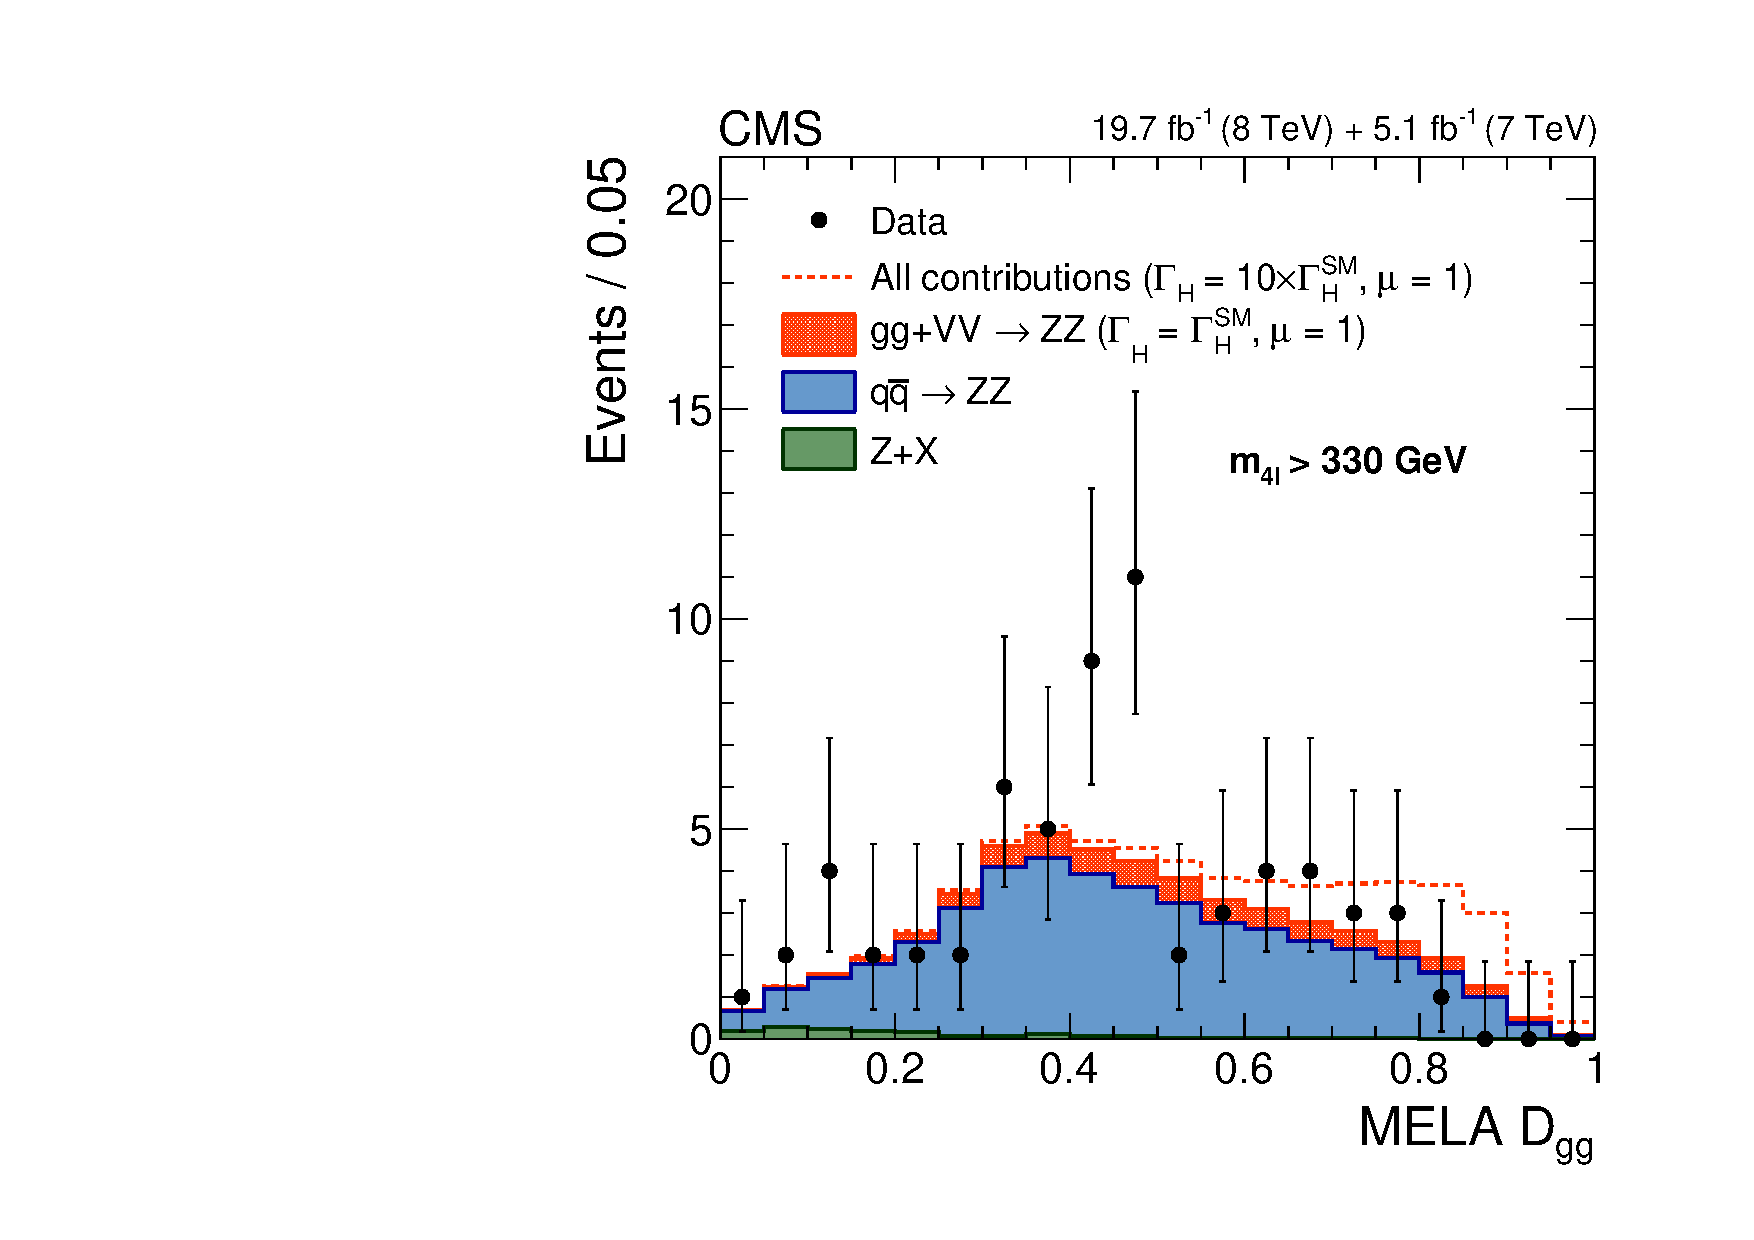
\includegraphics[width=.45\linewidth]{HiggsProperties/figures/fig3b_new.pdf}
\caption[$m_{4\ell}$ and $\mathcal{D}_{gg}$ Distributions of Expected and Observed $4\ell$ Events in the Off-Shell Signal-Enhanced Region]{Observed $4\ell$ events with SM expectations in signal-enriched region. Expectations for $gg+VV\rightarrow 4\ell$, including signal, background, and interference for a SM-like ($r=1$) Higgs boson width, are in filled red. Expectations for $gg+VV\rightarrow 4\ell$ with $r=10$ are plotted in dashed red. Irreducible $q\bar{q}\rightarrow 4\ell$ (blue) and reducible $Z+X$ (green) backgrounds are also plotted. On left, $m_{4\ell}$ distribution shows that there are few high mass events in signal-enriched region. On right, $\mathcal{D}_{gg}$ distribution shows that what high mass events exist are typically at lower values of $\mathcal{D}_{gg}$.}
\label{fig:Width4l_SignalEnriched}
\end{center}
\end{figure}

As there are no observed broad excesses, we can set an upper limit on the width of the Higgs boson. Letting $\mu_V$ and $\mu_F$ float, the expected exclusion limit at 95\% CL is $\Gamma_{H}<41.9$ $\rm{MeV}$. With all systematic uncertainties included, the observed exclusion limit is $\Gamma_{H} < 33.3$ $\rm{MeV}$. This result was further combined with an off-shell analysis in the $ZZ \rightarrow 2\ell2\nu$ channel\footnote{The $ZZ \rightarrow 2\ell2\nu$ channel has considerably worse mass resolution than $4\ell$ because of the missing energy of the neutrinos, but when combined with on-shell information from $4\ell$ its comparatively higher cross section (see Fig.~\ref{fig:HXSWGDecay}) leads to a powerful off-shell analysis.} to find a combined expected limit of $\Gamma_{H} < 33$ $\rm{MeV}$ at 95\% CL compared to the observed limit of $\Gamma_{H} < 22$ $\rm{MeV}$. These individual and combined limits can be seen in Fig.~\ref{fig:WidthLimits}. The combined best fit value for the Higgs width is $\Gamma_{H} = 1.8^{+7.7}_{-1.8}$ $\rm{MeV}$, in agreement with the Standard Model width of $4.15$ $\rm{MeV}$ for $m_{H}=125.6$ $\rm{GeV}$. These limits are substantially stronger than the $\Gamma_H < 3.4$ $\rm{GeV}$ measurement made only using on-shell information.

\begin{figure}[htbp]
\begin{center}
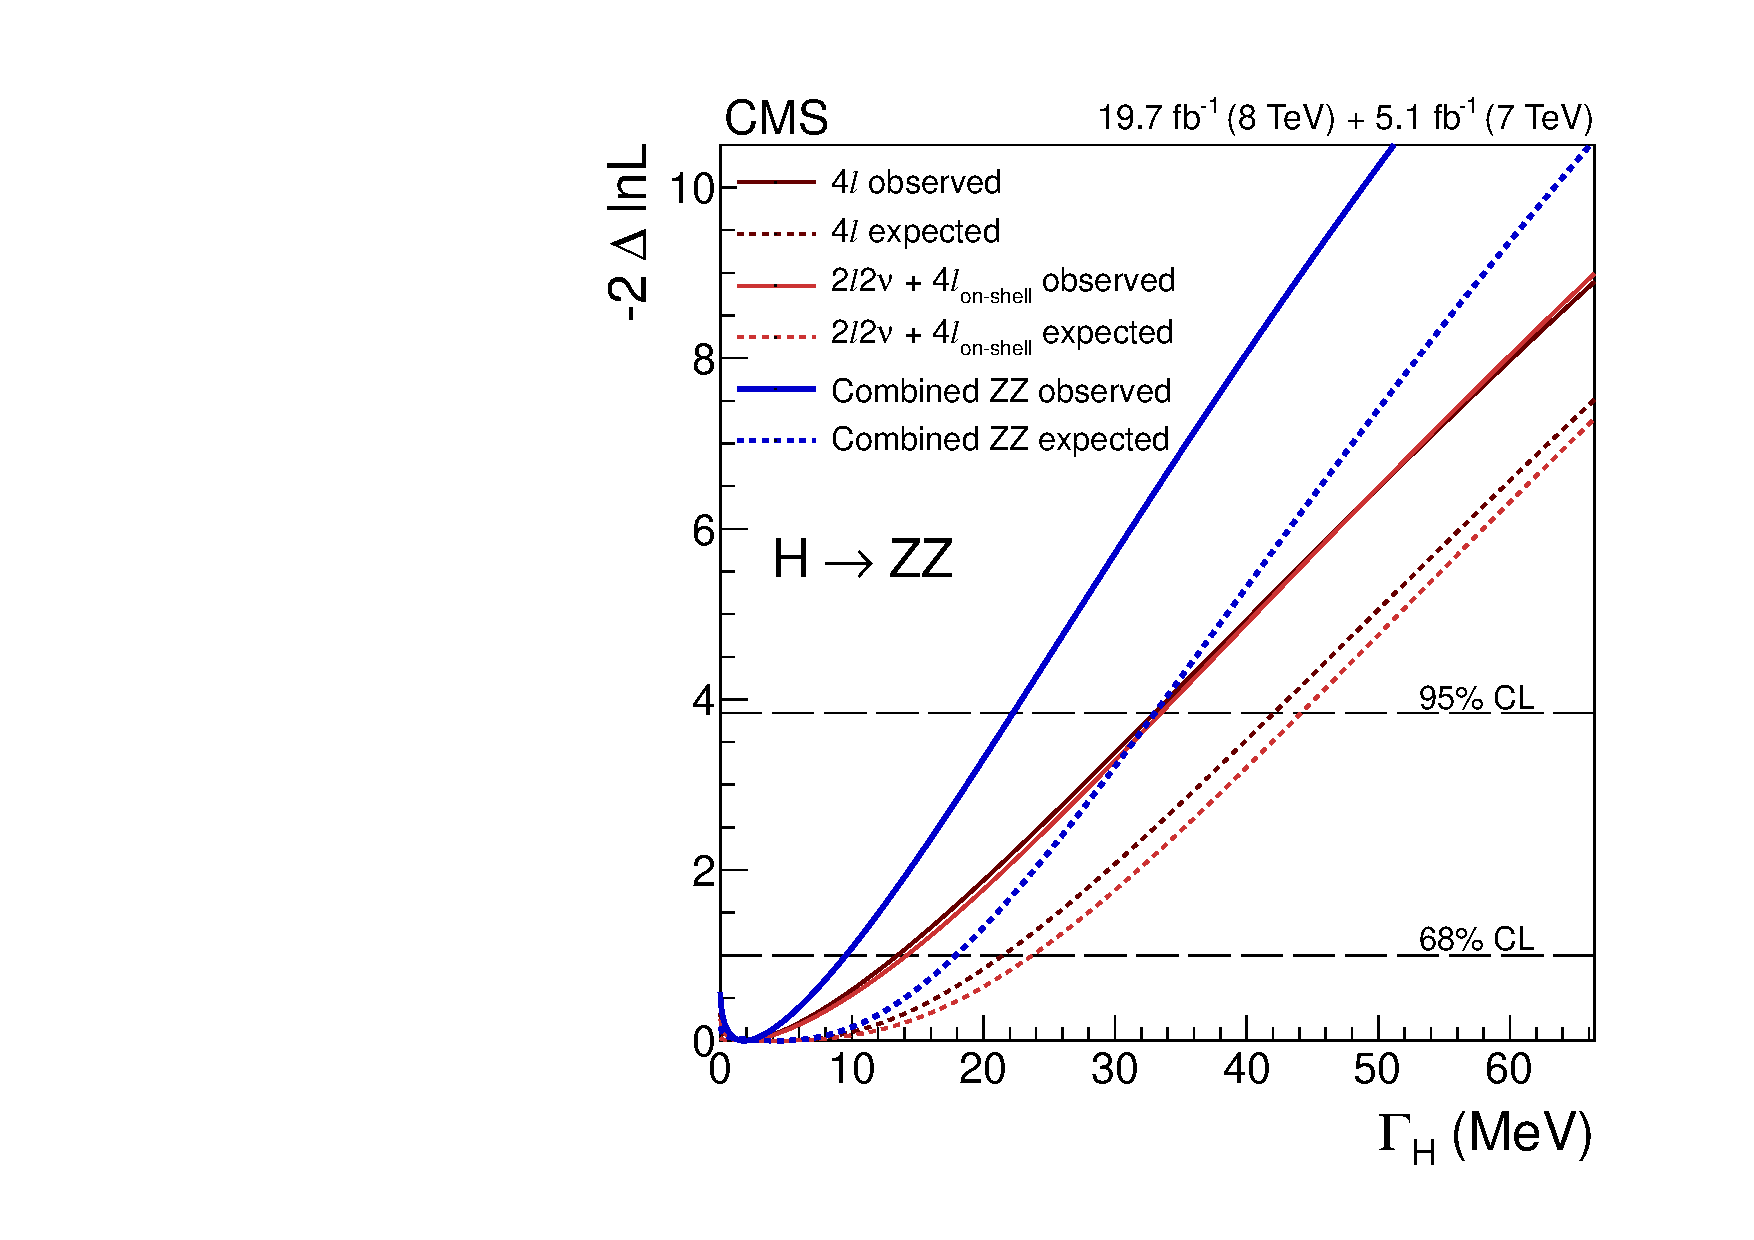
\includegraphics[width=.8\linewidth]{HiggsProperties/figures/fig5_new.pdf}
\caption[Expected and Observed Limits on Higgs Width]{Expected (dashed) and observed (solid) likelihood scans for Higgs boson width for $m_{H}=125.6$ $\rm{GeV}$ using the full $4\ell$ mass range (dark red), the $2\ell2\nu$ channel off-shell mass range with $4\ell$ on-shell (light red), and combined (blue). In both channels, a dearth of events is observed leading to a tighter observed limit at 95\% CL, $\Gamma_{H} < 22$ $\rm{MeV}$, than the expected $\Gamma_{H} < 33$ $\rm{MeV}$.}
\label{fig:WidthLimits}
\end{center}
\end{figure}

\section{Off-Shell Anomalous Coupling}
\label{sec:OffShellAnom}

The width analysis using the off-shell region in Sec.~\ref{sec:Width} relies on two small theoretical assumptions: i) the observed Higgs boson has standard model couplings and ii) the coupling ratios between on-shell and off-shell are well modeled. The first assumption appears to be valid given current measurements. As shown in the results of Sec.~\ref{sec:SpinParity}, the Higgs boson is observed to be in agreement with a scalar. The second assumption implies that the fermionic loop of gluon-gluon fusion is dominated by the top quark and there are no BSM particles that contribute to its production. In Sec.~\ref{sec:HighMass}, no Higgs-like resonances were observed in the high mass region and no search \cite{Agashe:2014kda} for fermions beyond the top-mass has found a higher mass particle.

For the couplings, although anomalous couplings do not have a substantial effect on the on-shell normalization, they do alter the overall cross section seen in the off-shell region. Using {\tt MCFM} and MELA, simulations of anomalous couplings, seen in Fig.~\ref{fig:MCFMOffShellBSM}, will tend to give higher off-shell yields than the Standard Model, which would lead to an even tighter limit on the width. In particular, $f_{\Lambda Q}$, defined in Eqn.~\ref{eqn:fLQ}, is the most extreme off-shell enhancement and represents the scale of BSM physics that modifies the $HVV$ vertex. Furthermore, this anomalous coupling can \textit{only} be measured through this off-shell enhancement as all kinematic distributions become identical to the SM. By modifying the off-shell analysis of Sec.~\ref{sec:OffShellAnalysis}, we can simultaneously measure the final anomalous coupling of Eqn.~\ref{eq:scalarAmpl_wformfactors} and loosen the assumptions in the width measurement.

\begin{figure}[htbp]
\begin{center}
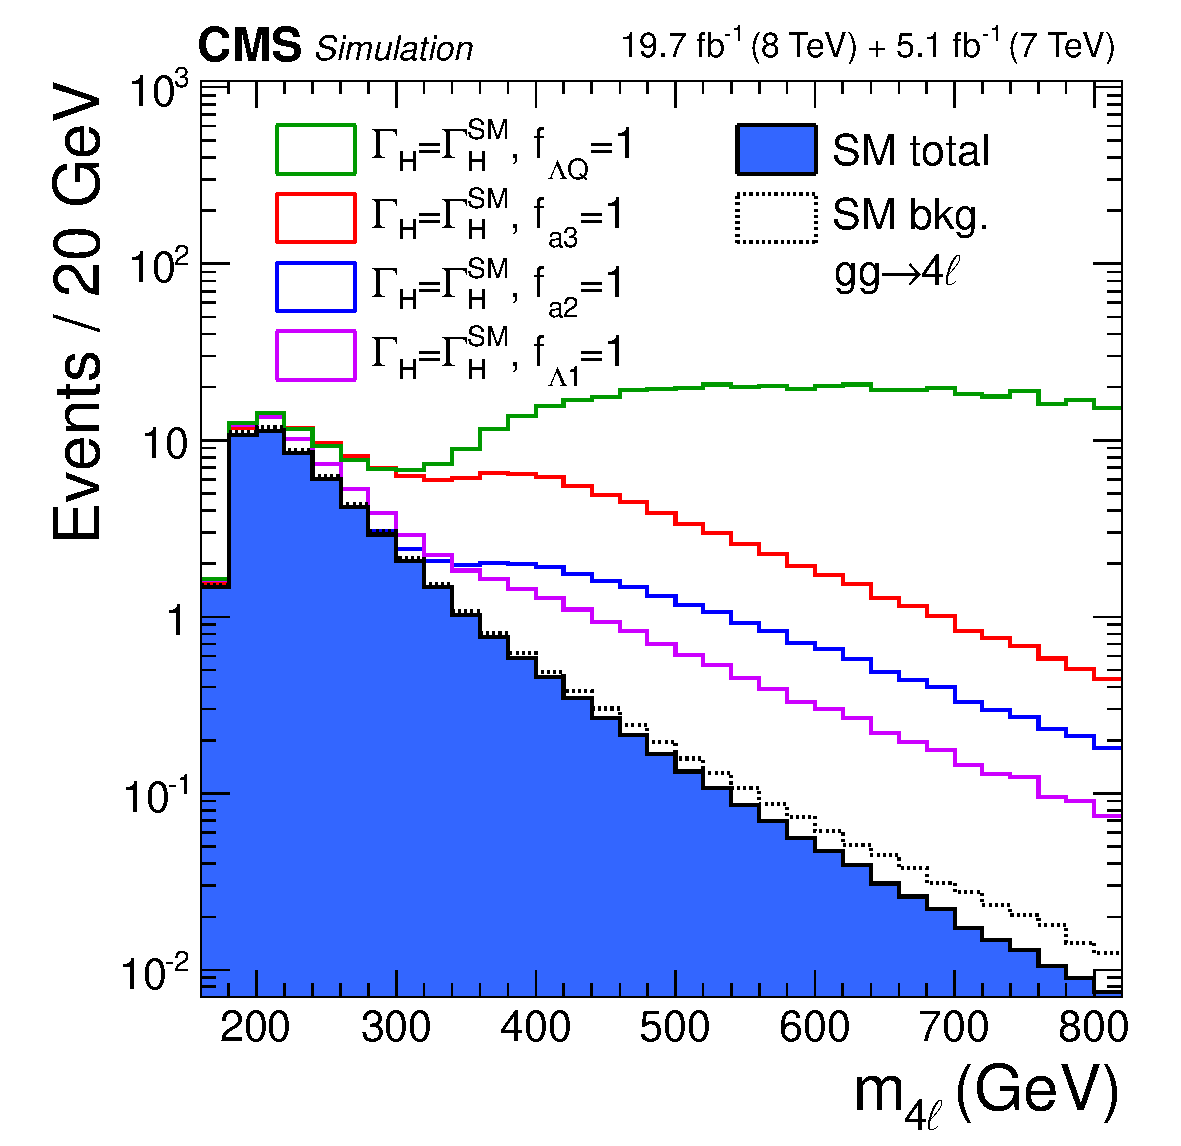
\includegraphics[width=.7\linewidth]{HiggsProperties/figures/cCanvas_MCFMBSM_GenLevel_new.pdf}
\caption[Simulated Off-shell Enhancements in the $4\ell$ Channel from Anomalous $HVV$ Couplings]{Compared to the SM off-shell yields in $4\ell$ (total $gg\rightarrow 4\ell$ in filled blue, background only in dotted black), anomalous couplings will tend to give considerable enhancements. Modeled using {\tt MCFM} and MELA anomalous couplings, $f_{\Lambda Q}=1$ (green), $f_{a3}=1$ (red), $f_{a2}=1$ (blue), and $f_{\Lambda 1}=1$ (magenta) were generated for demonstration of these effects. Arbitrary anomalous couplings can be generated and $f_{\Lambda Q}=1$ is the most extreme enhancement compared to SM.}
\label{fig:MCFMOffShellBSM}
\end{center}
\end{figure}

Because $f_{\Lambda Q}\neq0$ will have the same kinematic distributions as $f_{\Lambda Q}=0$, the off-shell analysis can be adapted simply by modifying the $m_{4\ell}$ distributions of the $(m_{4\ell},\mathcal{D}_{gg})$ templates to reflect the value of $f_{\Lambda Q}$. This reweighting can be done using the following equations\footnote{Where the phase $\phi_{\Lambda Q}=0$ or $\pi$, where the coupling would be real.}:
\begin{align}
{\mathcal P}_{\rm sig}^{\rm gg} &= \left|\sqrt{1-f_{\Lambda Q} } - \sqrt{f_{\Lambda Q}} \,e^{i\phi_{\Lambda Q}} \cdot \frac{m_{ZZ}^2}{m_{H}^2}\right|^2\cdot {\mathcal P}_{\rm sig}^{\rm gg}(\rm SM) \notag \\
{\mathcal P}_{\rm int}^{\rm gg} &= Re \left(\sqrt{1-f_{\Lambda Q} } - \sqrt{f_{\Lambda Q} } \,e^{i\phi_{\Lambda Q}} \cdot \frac{m_{ZZ}^2}{m_{H}^2}\right) \cdot {\mathcal P}_{\rm int}^{\rm gg}(\rm SM) \notag \\
{\mathcal P}_{\rm sig}^{\rm VBF} &= \left|\sqrt{1-f_{\Lambda Q} } - \sqrt{f_{\Lambda Q} } \,e^{i\phi_{\Lambda Q}} \cdot \frac{m_{ZZ}^2}{m_{H}^2}\right|^4\cdot {\mathcal P}_{\rm sig}^{\rm VBF}(\rm SM) \notag \\
{\mathcal P}_{\rm int}^{\rm VBF} &= \left|\sqrt{1-f_{\Lambda Q} } - \sqrt{f_{\Lambda Q} } \,e^{i\phi_{\Lambda Q}} \cdot \frac{m_{ZZ}^2}{m_{H}^2}\right|^2\cdot {\mathcal P}_{\rm int}^{\rm VBF}(\rm SM) \notag
\label{eqn:fLQOffShellFormula} 
\end{align}
Note that for VBF, because there are two $HVV$ vertices -- one in production and one in decay -- the $f_{\Lambda Q}$ enhancement is two powers stronger for VBF signal than ggF signal. For large values of $m_{ZZ}$, the $\sqrt{f_{\Lambda Q}}$ term will dominate unless $f_{\Lambda Q}$ is very small. This implies that we should expect a very narrow limit on $f_{\Lambda Q}$ as no $4\ell$ event is observed for $m_{4\ell} > 800$ $\rm{GeV}$.

For the earlier width measurement, the limit was set using the total number of off-shell events with a separation of Higgs boson signal from background using decay kinematics. With the stronger off-shell enhancement being for VBF, we should again implement production separation in the off-shell region. In Sec.~\ref{sec:ZZ4lDjet}, a jet categorization determined which production discriminant ($p_T \rm{~or~} \mathcal{D}_{\rm jet}$) to use on events in the on-shell likelihood. For the off-shell region, instead of using the jet categorization, we implement a new categorization built on vbfMELA. Looking at the $\mathcal{D}_{\rm jet}$ distributions of VBF against either ggF or $q\bar{q}ZZ$ in Fig.~\ref{fig:vbfMELATemplates}, we categorize events by their value of $\mathcal{D}_{\rm jet}$ with one category for events with $\mathcal{D}_{\rm jet}\geq0.5$ and the other category with $\mathcal{D}_{\rm jet}<0.5$ or having less than two jets. The full list of observables and categories for the on-shell and off-shell regions is in Table~\ref{tbl:OffShellCatsAndObervs}.

\begin{table}[htb]
\begin{center}
\begin{tabular}{cccccc}
\hline
Category & $m_{4\ell}$ & Jets & \multicolumn{3}{c}{Observables $\vec{x}$} \\
\hline
\hline
On-shell Dijet & $105.6<m_{4\ell}<140.6$ $\rm{GeV}$ & $N_{\rm jet}\ge2$ & $m_{4\ell}$ & ${\mathcal D}^{\rm kin}_{\rm bkg}$ & ${\mathcal{D}}_{\rm jet}$ \\
On-shell Non-Dijet & $105.6<m_{4\ell}<140.6$ $\rm{GeV}$ & $N_{\rm jet}<2$ & $m_{4\ell}$ & ${\mathcal D}^{\rm kin}_{\rm bkg}$ & ${p}_{\rm T}$ \\
Off-shell Dijet & $220<m_{4\ell}<1600$ $\rm{GeV}$ & ${\mathcal{D}}_{\rm jet}\geq0.5$ & $m_{4\ell}$ & $\mathcal{D}_{gg}$ &  \\
Off-shell Non-Dijet & $220<m_{4\ell}<1600$ $\rm{GeV}$ & ${\mathcal{D}}_{\rm jet}<0.5$ or $N_{\rm jet}<2$ & $m_{4\ell}$ & $\mathcal{D}_{gg}$ &  \\
\hline
\end{tabular}
\caption[Categorizations and Observables Used in On-shell and Off-shell Regions of $f_{\Lambda Q}$ Measurement]{On-shell and off-shell jet categorizations and observables used for likelihood analysis. On-shell region is identical to method of Sec.~\ref{sec:ZZ4lAnalysis} near $m_{H}=125.6$ $\rm{GeV}$ except that vbfMELA is used for $\mathcal{D}_{\rm jet}$ as in Sec.~\ref{sec:HighMass}. Off-shell region is identical to method used in Sec.~\ref{sec:OffShellAnalysis}, with added jet categorization based on $\mathcal{D}_{\rm jet}$.}
\label{tbl:OffShellCatsAndObervs}
\end{center}
\end{table}

The $\mathcal{D}_{\rm jet}\geq0.5$ category will be remarkably pure in VBF, where less than 5\% of ggF or background events pass this threshold compared to about 40\% of VBF events, as seen in the ratios of Fig.~\ref{fig:DjetRatios}. Given that these ratios are very small for all but VBF, the $(m_{4\ell},\mathcal{D}_{gg})$ templates for each category are built using the full MC or control region then scaled by analytic $m_{4\ell}$ fits of the $\mathcal{D}_{\rm jet}>0.5$ ratio to give the appropriate normalization. VBF has sufficient statistics in each category to build separate templates from each subset of simulated events.

For VBF and $q\bar{q}$, the nominal $\mathcal{D}_{\rm jet}$ ratios come from the respective MC samples that were used in the earlier off-shell analysis. For ggF, as discussed in Sec.~\ref{sec:HighMass}, the jet kinematics of {\tt MINLO} is more accurate than {\tt POWHEG} or other LO generators, so the nominal ratio used for categorization is found from {\tt MINLO}. In implementing the $\mathcal{D}_{\rm jet}>0.5$ selection, we studied the effects of using alternative MC for the purpose of adding a yield systematic for the jet categorization. For VBF, {\tt Phantom} and {\tt JHUGen} at LO were compared to {\tt POWHEG} at NLO. The relative uncertainty in the yield of the $\mathcal{D}_{\rm jet}>0.5$ category is about 5\%. Similar studies were done in ggF ({\tt MCFM} and {\tt GG2VV} at LO, {\tt POWHEG} and {\tt MINLO} at NLO) and $q\bar{q}ZZ$ ({\tt POWHEG} at NLO and {\tt MadGraph} for an inclusive sample with up to 2 jets), where relative yield uncertainties were found to be 15\% and 25\%, respectively. $Z+X$ is data driven, so the nominal shape comes from the control region with a conservative 100\% uncertainty on the dijet yield. These new yield uncertainties\footnote{The considered shape uncertainties of $\mathcal{D}_{\rm jet}$ in Sec.~\ref{sec:ZZ4lDjet} can be reinterpreted as yield uncertainties for the $\mathcal{D}_{\rm jet}>0.5$ categorization. The largest available deviations come from different MC generators.} are 100\% anti-correlated between the non-dijet and dijet categorizations to maintain the same total normalization.

\begin{figure}[htbp]
\begin{center}
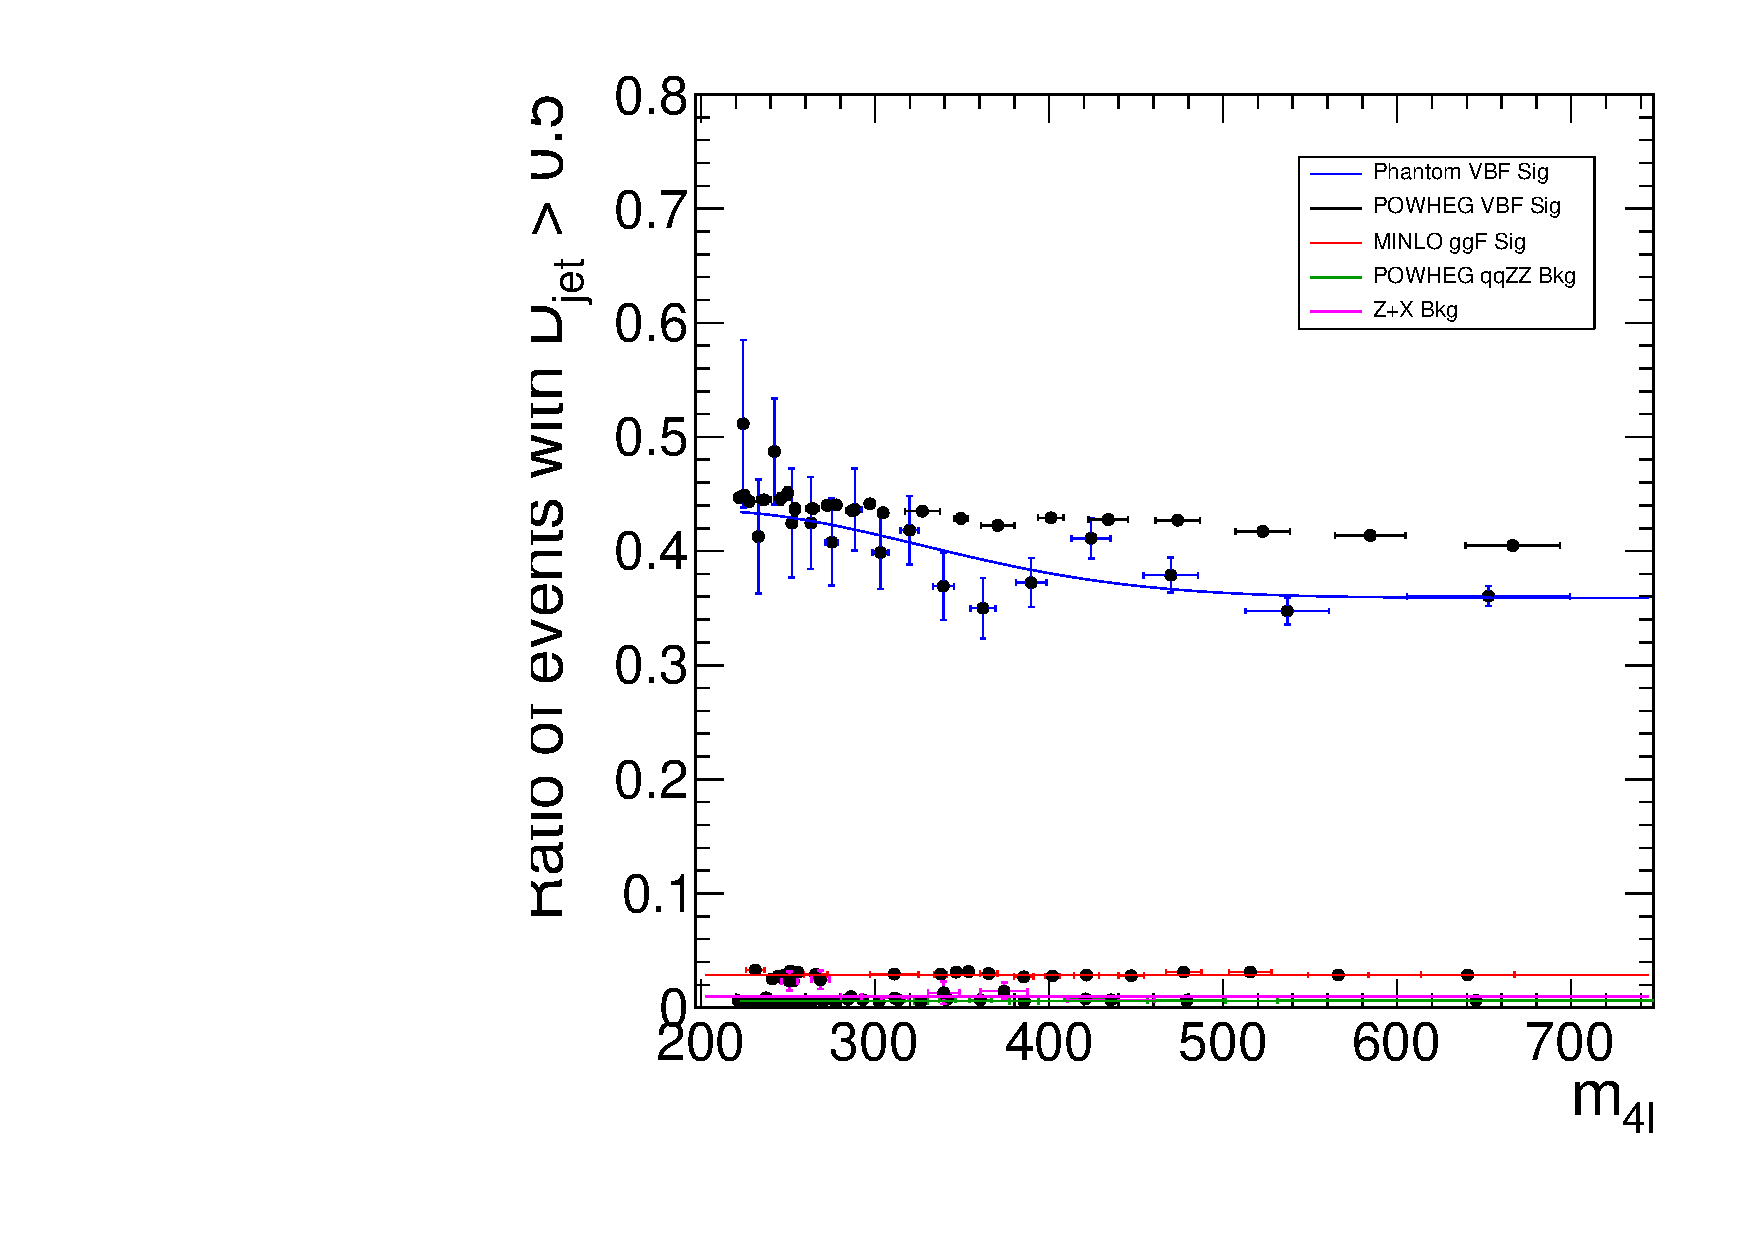
\includegraphics[width=.7\linewidth]{HiggsProperties/figures/DjetCutShapeOverlay_8TeV_Sig+Bkg_all.pdf}
\caption[$\mathcal{D}_{\rm jet}>0.5$ Ratios for Production Separation in $f_{\Lambda Q}$ Measurement]{Ratios of events that pass $\mathcal{D}_{\rm jet}>0.5$ categorization over total number of events. VBF (blue) has the highest ratios, around 40\% over a wide $m_{4\ell}$ range. ggF (magenta), $Z+X$ (green), and $q\bar{q}ZZ$ (red) all have much lower ratios, sub 5\%. Aside from VBF, these ratios are fit analytically to build templates for each category.}
\label{fig:DjetRatios}
\end{center}
\end{figure}

Other than the new jet categorization using vbfMELA to isolate the elevated impact on VBF and the modification of the templates for values of $f_{\Lambda Q}$, there are only small changes from the analysis of Sec.~\ref{sec:OffShellAnalysis}. For VBF, the {\tt Phantom} samples were fully simulated through the detector by the time of this analysis, so they are used for creating the templates with a minor reweighting. VH is a small contribution (about 10-15\% relative to VBF for $m_{4\ell}\gtrsim200$ $\rm{GeV}$) in the off-shell region and these {\tt Phantom} samples include its contribution, but only when the associated $W$ or $Z$ decays hadronically. A small reweighting is applied to account for the additional leptonic decays.

With these changes in place, we still have the same $m_{4\ell}$ distributions as in Fig.~\ref{fig:Width4l_Full}, but we also plot the $m_{4\ell}$ distributions separately for each jet categorization. In the left plot of Fig.~\ref{fig:OffShell_Categorized}, we have applied a $\mathcal{D}_{gg} > 0.67$ selection to emphasize the signal-enriched region. As with Fig.~\ref{fig:Width4l_SignalEnriched}, there are few signal-like events in the off-shell region, which led to the upper limit measurement on the width. When $f_{\Lambda Q}$ is small, destructive interference will bring down the contribution of an anomalously large width. However, as $f_{\Lambda Q}$ increases, the number of signal-like events expected at very high masses ($m_{4\ell}>800$ $\rm{GeV}$) increases, most obviously in the $\mathcal{D}_{\rm jet}>0.5$ category in the right plot of Fig.~\ref{fig:OffShell_Categorized}.

\begin{figure}[htbp]
\begin{center}
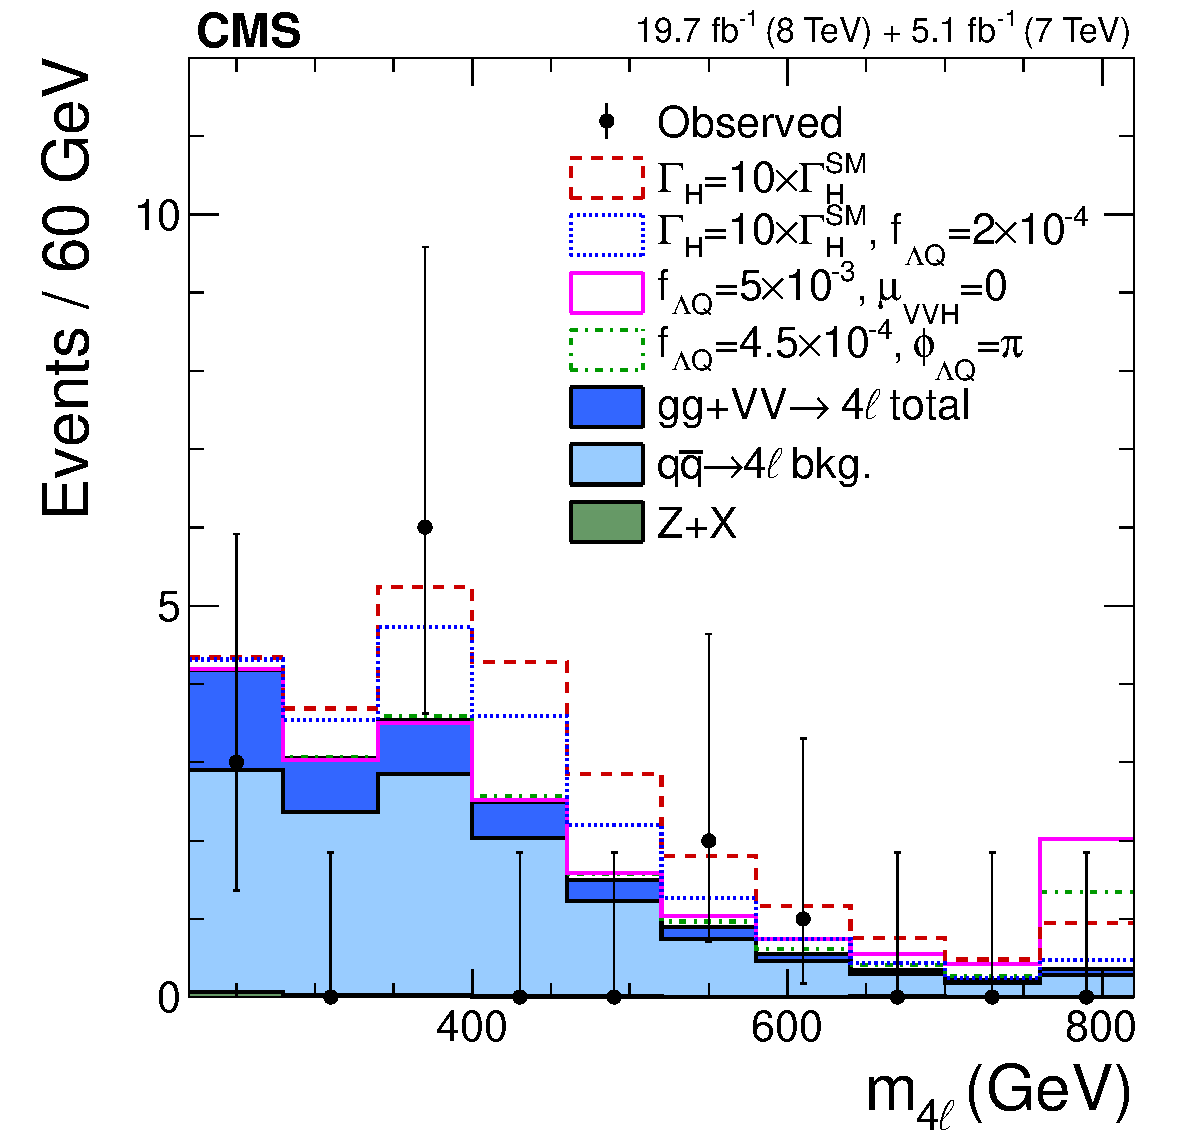
\includegraphics[width=.45\linewidth]{HiggsProperties/figures/nonDjet_m4l_Enhanced_Dgg0p67_new.pdf}
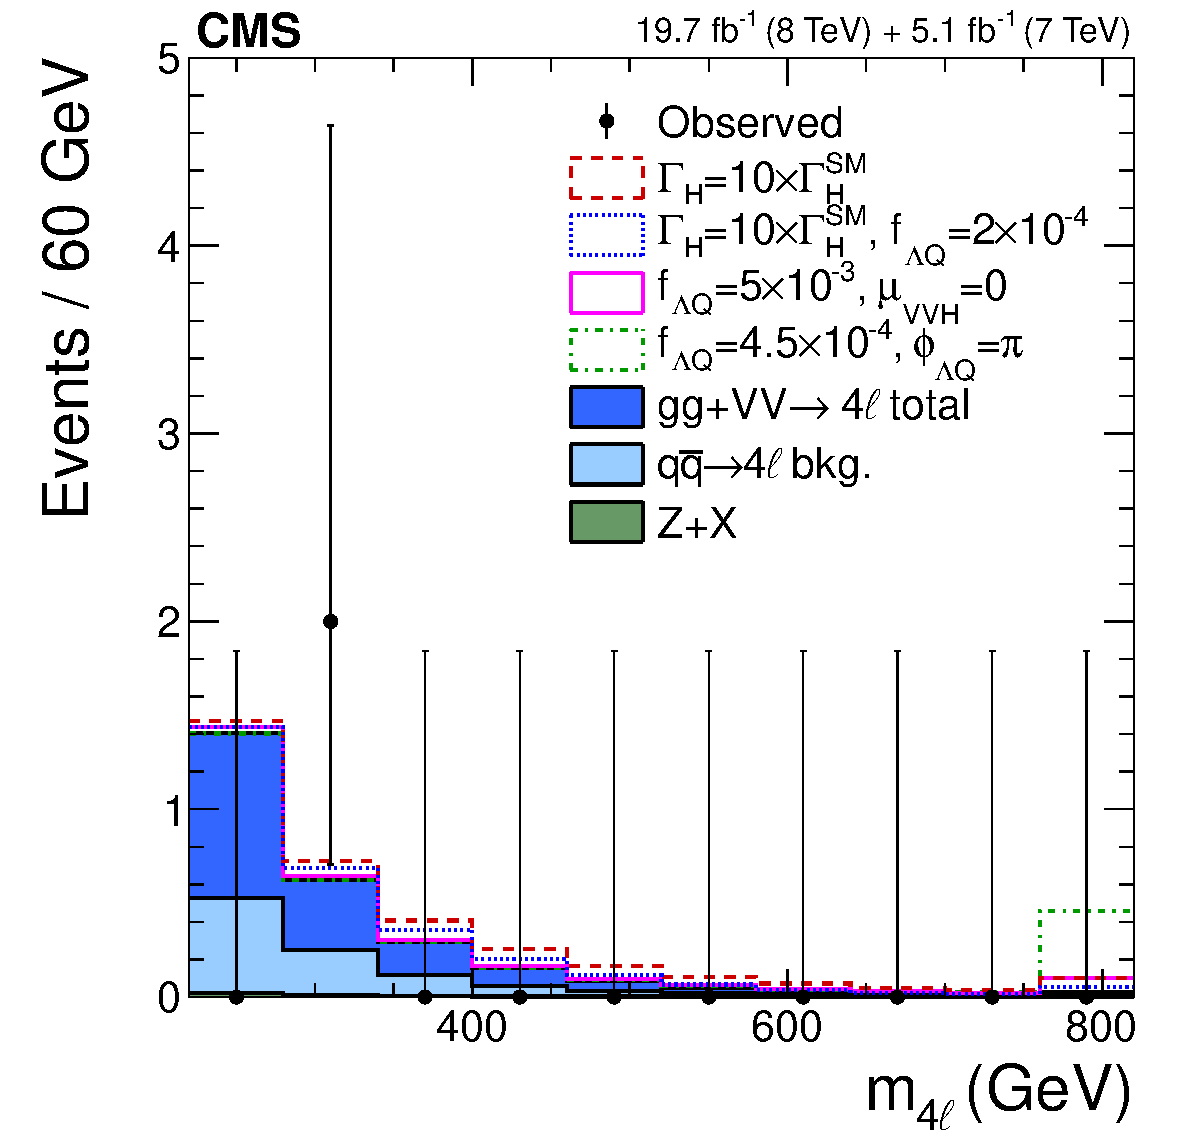
\includegraphics[width=.45\linewidth]{HiggsProperties/figures/Djet_m4l_new.pdf}
\caption[$m_{4\ell}$ Distributions of Jet Categorized Expected and Observed $4\ell$ Events in the Off-Shell Region for $f_{\Lambda Q}$ Measurement]{Observed $4\ell$ events (black points) for off-shell regions, $220<m_{4\ell}<800$ $\rm{GeV}$ where the last bin of the histogram also includes yields for $800<m_{4\ell}<1600$ $\rm{GeV}$, with expected distributions with SM-like Higgs boson. $gg + VV \rightarrow 4\ell$ distributions (dark blue) account for signal, background, and interference for ggF and VBF \& VH production methods. $q\bar{q}\rightarrow ZZ$ (light blue) and $Z+X$ (green) are the dominant and sub-dominant backgrounds. Four BSM contributions are also shown: $\Gamma_H=10\times\Gamma_{SM}$ with $f_{\Lambda Q}=0$ (dashed red) and $f_{\Lambda Q}=2\times10^{-4}$ (dotted blue) show an enhancement just past the $2\times m_{Z}$ peak whereas for the $f_{\Lambda Q}$ close to the expected exclusion limits, $\Gamma_{H}=\Gamma_{SM}$ with $f_{\Lambda Q}=5\times10^{-3}$ (solid magenta) and $f_{\Lambda Q}\times\cos(\phi_{\Lambda Q})=-4.5\times10^{-4}$, the enhancement is almost entirely in $m_{4\ell}>800$ $\rm{GeV}$. On left, $\mathcal{D}_{gg} > 0.67$ and $\mathcal{D}_{\rm jet}<0.5$ or $N_{jets}<2$. On right, $\mathcal{D}_{\rm jet}\geq0.5$.}
\label{fig:OffShell_Categorized}
\end{center}
\end{figure}

The impact of the destructive interference for small values of $f_{\Lambda Q}$ means that the width limit will loosen somewhat when $f_{\Lambda Q}$ is allowed to vary. This is exactly what is seen in Fig.~\ref{fig:WidthLimitsWithfLQ}, where the likelihood scans were run both using $f_{\Lambda Q}=0$ -- identical to Sec.~\ref{sec:WidthResults} -- and when we unconstrain $f_{\Lambda Q}$. The expected and observed limits for $f_{\Lambda Q}=0$ are $\Gamma_H < 41$ $\rm{MeV}$ and $\Gamma_H < 26$ $\rm{MeV}$, respectively. When $f_{\Lambda Q}$ is unconstrained, the expected upper limit becomes $\Gamma_H < 73$ $\rm{MeV}$ with an observed upper limit of $\Gamma_H < 46$ $\rm{MeV}$, where all limits are at 95\% CL.

\begin{figure}[htbp]
\begin{center}
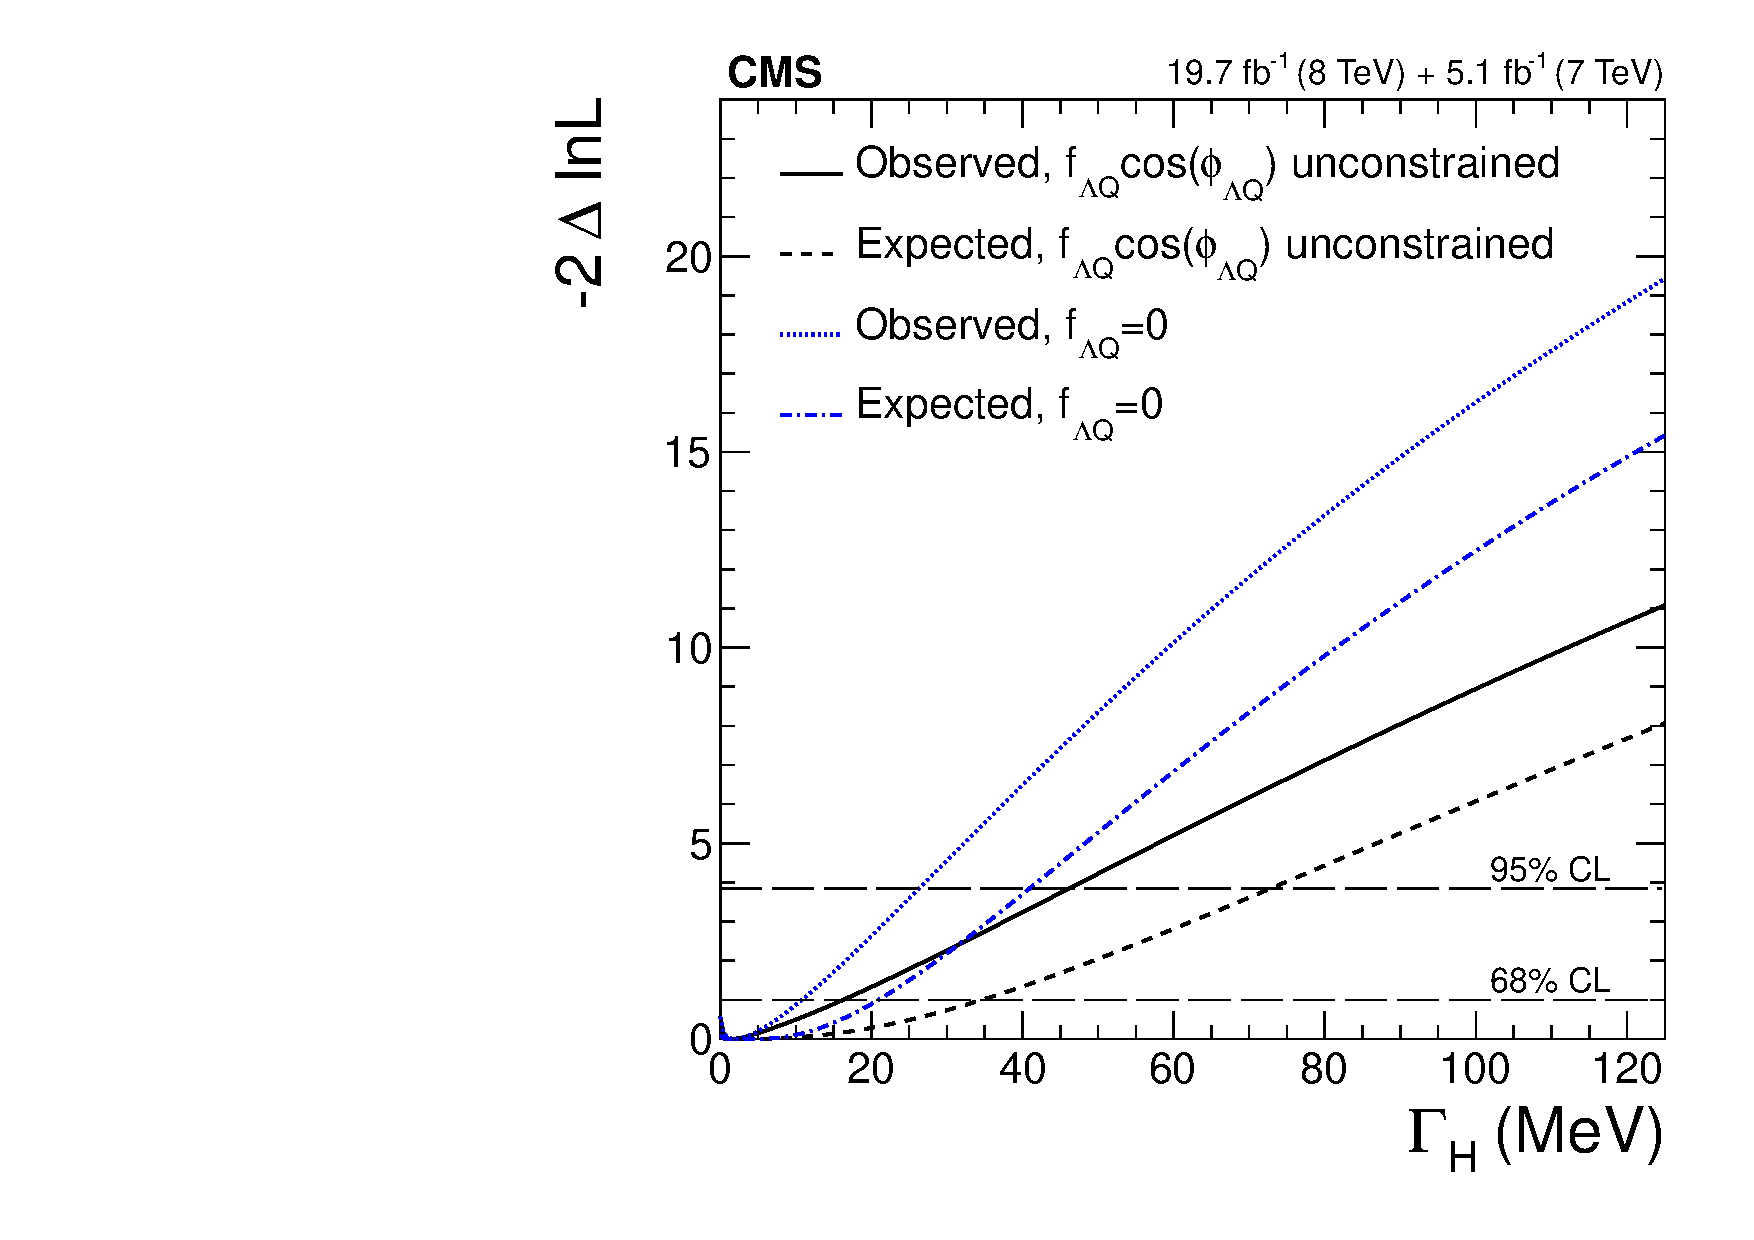
\includegraphics[width=.9\linewidth]{HiggsProperties/figures/width_1DScan_GGsm.pdf}
\caption[Expected and Observed Limits on Higgs Boson Width with Anomalous Coupling]{Likelihood scans for Higgs boson width for $m_{H}=125.6$ $\rm{GeV}$ with $f_{\Lambda Q}$ anomalous coupling. When $f_{\Lambda Q}=0$, the results are similar to Sec.~\ref{sec:WidthResults} with expected (dot dashed blue) limit of $\Gamma_H < 41$ $\rm{MeV}$ compared to an observed (dotted blue) limit of $\Gamma_H < 26$ $\rm{MeV}$. When $f_{\Lambda Q}$ is allowed to float unconstrained, the width limits loosen giving an observed (solid black) limit of $\Gamma_H < 46$ $\rm{MeV}$ compared to the expected (dashed black) limit of $\Gamma_H < 73$ $\rm{MeV}$. All limits listed at 95\% CL.}
\label{fig:WidthLimitsWithfLQ}
\end{center}
\end{figure}

Alternatively, for a given value of the Higgs boson width, we can set limits on $f_{\Lambda Q}$. In Fig.~\ref{fig:fLQLimits}, we set $\Gamma_{H}=\Gamma_{SM}$. The expected value of $f_{\Lambda Q}\cos(\phi_{\Lambda Q})$ is\footnote{Recall that for this analysis, $\phi_{\Lambda Q}=0$ or $\pi$.} $0 ^{+10.7}_{-4.5} \times 10^{-4}$ with an observed best fit of $f_{\Lambda Q}\cos(\phi_{\Lambda Q}) = 0.1 ^{+10.5}_{-3.7} \times 10^{-4}$, so the $\Lambda_{Q}$ anomalous coupling is in agreement with the Standard Model expectations. The observed allowed region at 95\% CL is $[-24,38]\times 10^{-4}$ compared to the expected region of $[-36,44] \times 10^{-4}$. A limit of $f_{\Lambda Q}$ where $\Gamma_H$ is allowed to float unconstrained cannot be set because the off-shell behavior disappears entirely as $\Gamma_{H}\rightarrow0$. However, the 2D likelihood scan of $(\Gamma_{H},f_{\Lambda Q})$ has been constructed, seen in Fig.~\ref{fig:2DWidthScan}.

\begin{figure}[htbp]
\begin{center}
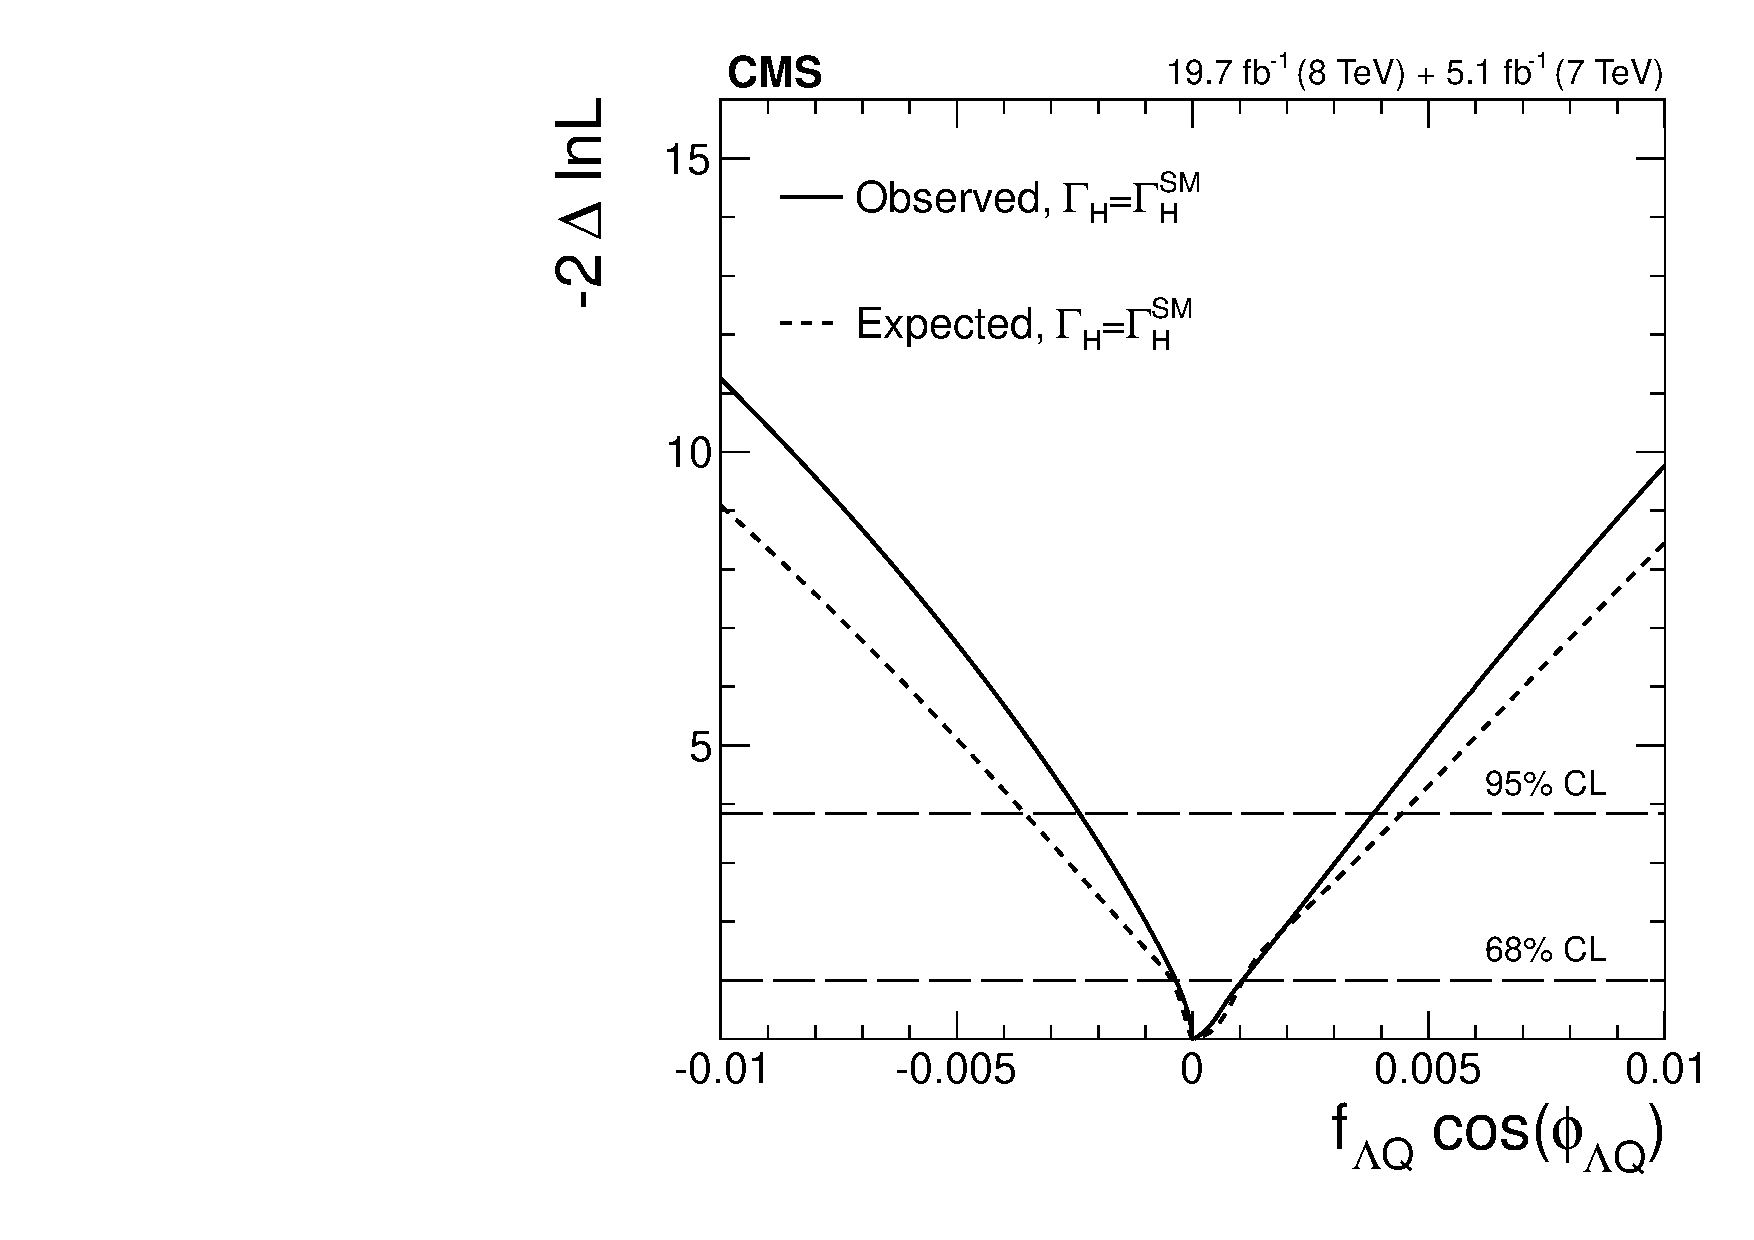
\includegraphics[width=.9\linewidth]{HiggsProperties/figures/width_1DScan_fLQ.pdf}
\caption[Expected and Observed Limits on $f_{\Lambda Q}\cos(\phi_{\Lambda Q})$]{Expected (dashed) and observed (solid) likelihood scans for $f_{\Lambda Q}\cos(\phi_{\Lambda Q})$ where $\Gamma_{H}=\Gamma_{H}^{SM}$. Expected allowed region at 95\% CL is $[-36,44] \times 10^{-4}$ compared to observed allowed region of $[-24,38]\times 10^{-4}$. Observed best fit value of $f_{\Lambda Q}\cos(\phi_{\Lambda Q})=0.1 ^{+10.5}_{-3.7} \times 10^{-4}$ agrees with SM expectations.}
\label{fig:fLQLimits}
\end{center}
\end{figure}

\begin{figure}[htbp]
\begin{center}
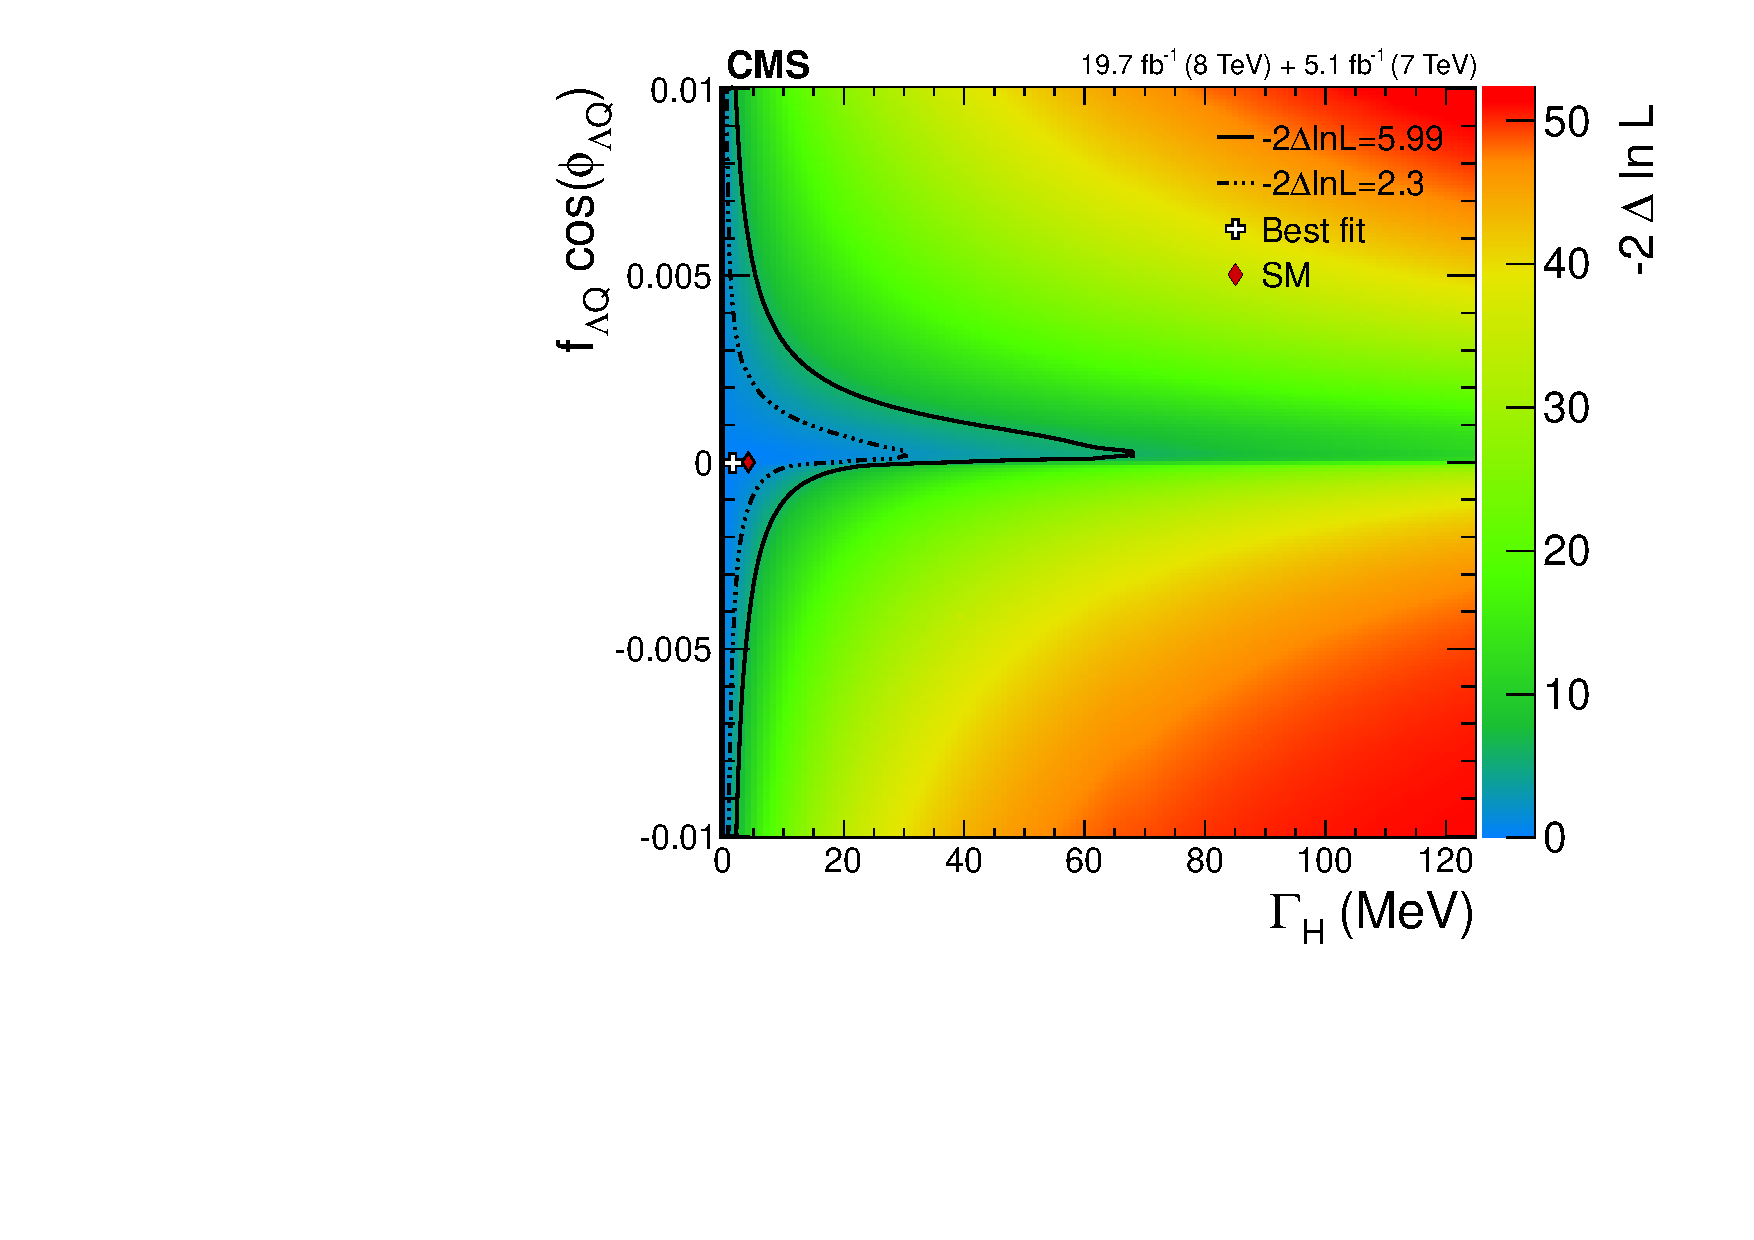
\includegraphics[width=.9\linewidth]{HiggsProperties/figures/width_2DScan_obs_2lnL.pdf}
\caption[2D $(\Gamma_{H},f_{\Lambda Q})$ Observed Likelihood Scan]{2D $(\Gamma_{H},f_{\Lambda Q})$ observed likelihood scan. SM expectation is plotted at the $(\Gamma_{SM},0)$ with a red rhombus compared to the observed best fit value at the white cross. Contour limits corresponding to 2D 68\% (dot dash line) and 95\% CL (solid line) are also plotted. For small values of $\Gamma_H$, the limit on $f_{\Lambda Q}$ weakens because $\Gamma_H\rightarrow0$ gives no expected off-shell signal events to be modified by $f_{\Lambda Q}$.}
\label{fig:2DWidthScan}
\end{center}
\end{figure}

This off-shell anomalous coupling measurement finishes the set of couplings for the $HVV$ vertex, where all couplings are observed to be in agreement with the Standard Model. Since the other couplings would similarly provide off-shell enhancement (see Fig.~\ref{fig:MCFMOffShellBSM}), the technique opens up further extensions to the on-shell spin-parity measurements, both in how they affect the width measurement and to how they could further constrain the anomalous coupling limits set in the on-shell region.

\section{Summary}
\label{sec:properties_summary}

After the discovery of a Higgs-like boson near $125$ $\rm{GeV}$, the Standard Model provides predictions for a variety of other properties the Higgs boson must exhibit: it should be a spin-0 CP-even scalar; its width should be around $4$ $\rm{MeV}$; it should have a small off-shell enhancement in the $H\rightarrow VV$ decay channels. In each case, these properties were measured and no anomalous couplings or widths or extra resonances were observed. However, this does not mean that the Higgs boson at $125.6$ $\rm{GeV}$ is The Higgs Boson of the Standard Model, it only implies that nothing anomalous has been observed yet. What, if anything, can we say about future measurements? Can we probe any of these properties further to find a deviation that would disagree with SM expectations and imply new physics?